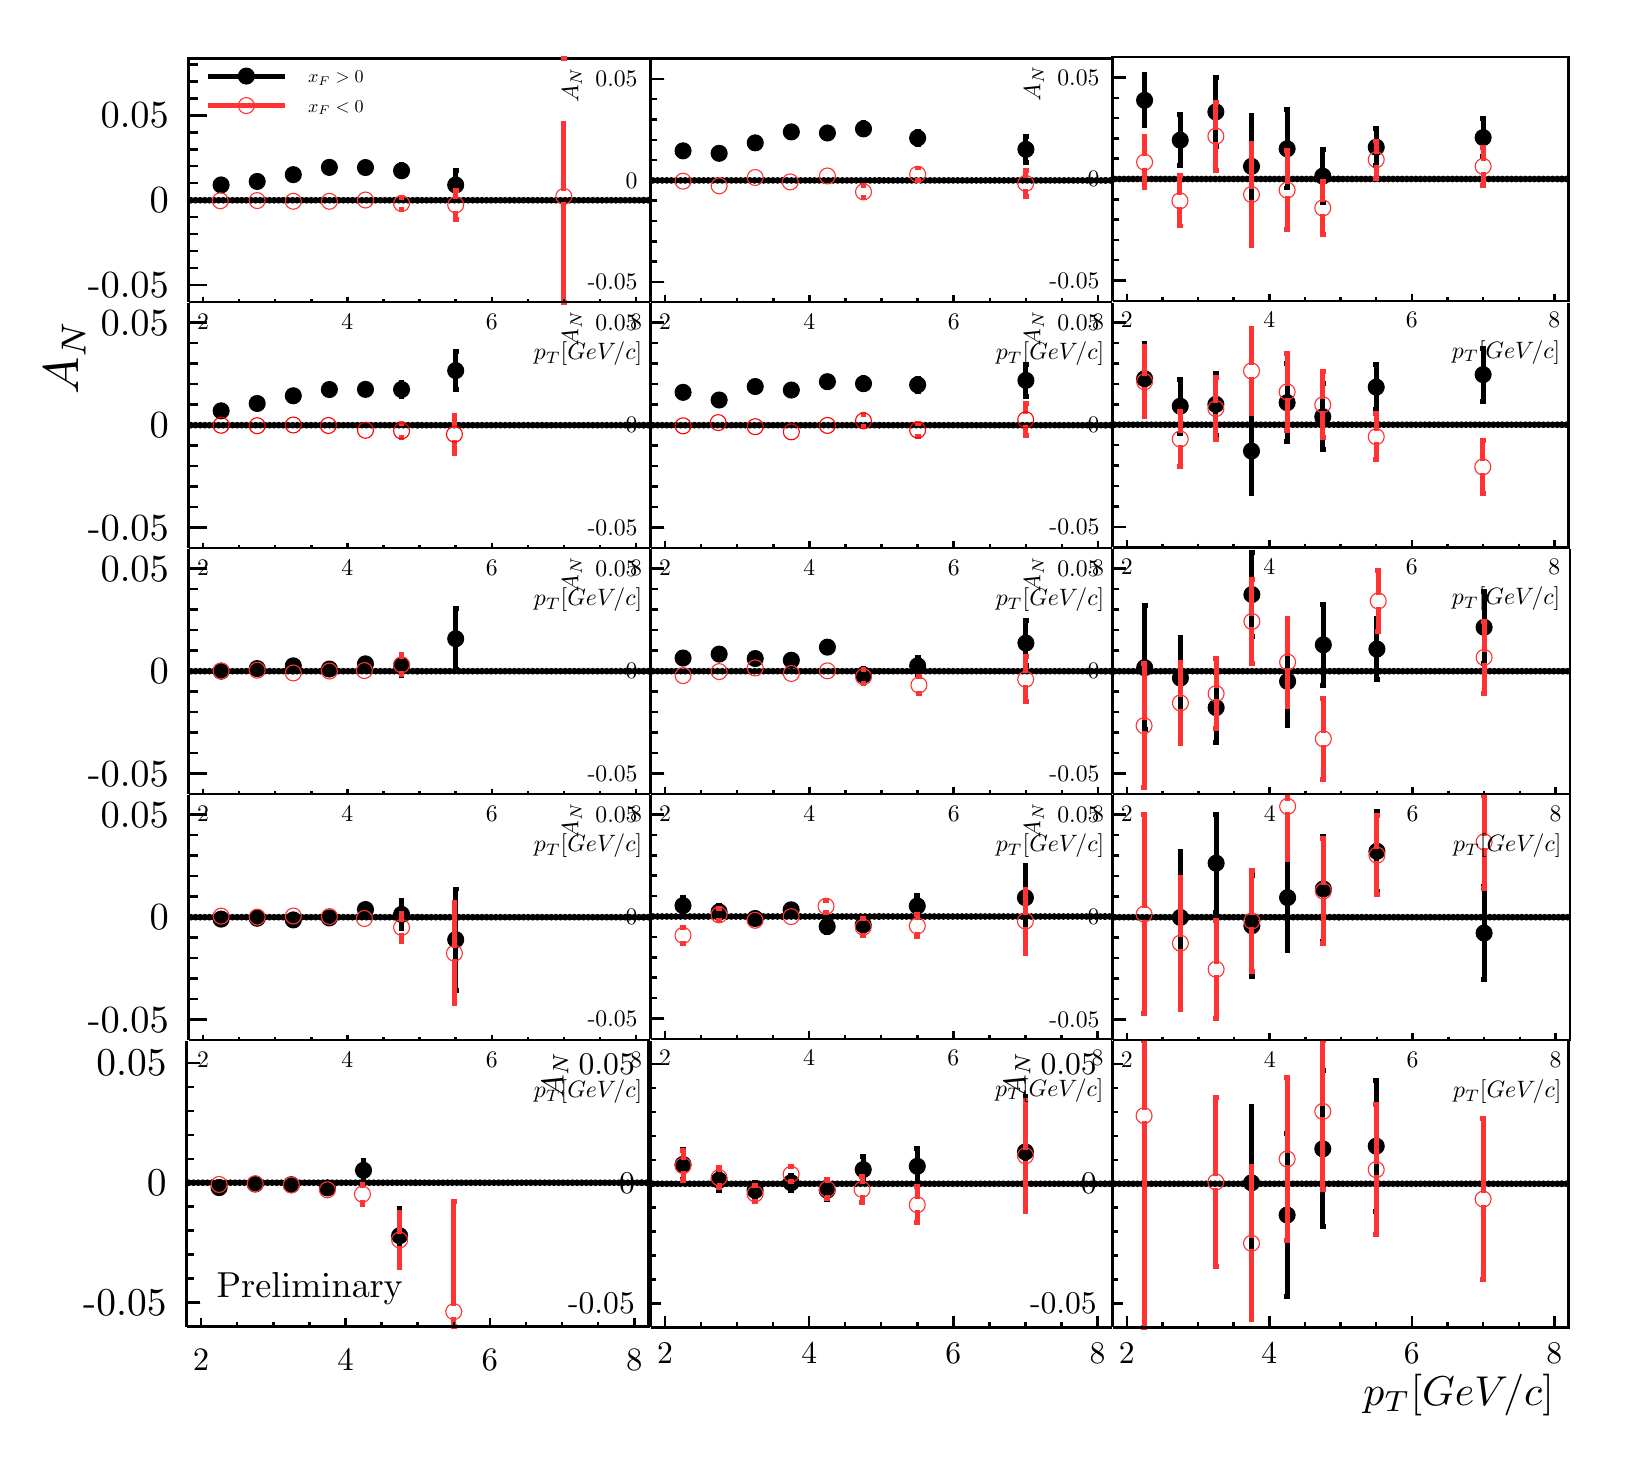
\begin{tikzpicture}
\pgfdeclareplotmark{cross} {
\pgfpathmoveto{\pgfpoint{-0.3\pgfplotmarksize}{\pgfplotmarksize}}
\pgfpathlineto{\pgfpoint{+0.3\pgfplotmarksize}{\pgfplotmarksize}}
\pgfpathlineto{\pgfpoint{+0.3\pgfplotmarksize}{0.3\pgfplotmarksize}}
\pgfpathlineto{\pgfpoint{+1\pgfplotmarksize}{0.3\pgfplotmarksize}}
\pgfpathlineto{\pgfpoint{+1\pgfplotmarksize}{-0.3\pgfplotmarksize}}
\pgfpathlineto{\pgfpoint{+0.3\pgfplotmarksize}{-0.3\pgfplotmarksize}}
\pgfpathlineto{\pgfpoint{+0.3\pgfplotmarksize}{-1.\pgfplotmarksize}}
\pgfpathlineto{\pgfpoint{-0.3\pgfplotmarksize}{-1.\pgfplotmarksize}}
\pgfpathlineto{\pgfpoint{-0.3\pgfplotmarksize}{-0.3\pgfplotmarksize}}
\pgfpathlineto{\pgfpoint{-1.\pgfplotmarksize}{-0.3\pgfplotmarksize}}
\pgfpathlineto{\pgfpoint{-1.\pgfplotmarksize}{0.3\pgfplotmarksize}}
\pgfpathlineto{\pgfpoint{-0.3\pgfplotmarksize}{0.3\pgfplotmarksize}}
\pgfpathclose
\pgfusepathqstroke
}
\pgfdeclareplotmark{cross*} {
\pgfpathmoveto{\pgfpoint{-0.3\pgfplotmarksize}{\pgfplotmarksize}}
\pgfpathlineto{\pgfpoint{+0.3\pgfplotmarksize}{\pgfplotmarksize}}
\pgfpathlineto{\pgfpoint{+0.3\pgfplotmarksize}{0.3\pgfplotmarksize}}
\pgfpathlineto{\pgfpoint{+1\pgfplotmarksize}{0.3\pgfplotmarksize}}
\pgfpathlineto{\pgfpoint{+1\pgfplotmarksize}{-0.3\pgfplotmarksize}}
\pgfpathlineto{\pgfpoint{+0.3\pgfplotmarksize}{-0.3\pgfplotmarksize}}
\pgfpathlineto{\pgfpoint{+0.3\pgfplotmarksize}{-1.\pgfplotmarksize}}
\pgfpathlineto{\pgfpoint{-0.3\pgfplotmarksize}{-1.\pgfplotmarksize}}
\pgfpathlineto{\pgfpoint{-0.3\pgfplotmarksize}{-0.3\pgfplotmarksize}}
\pgfpathlineto{\pgfpoint{-1.\pgfplotmarksize}{-0.3\pgfplotmarksize}}
\pgfpathlineto{\pgfpoint{-1.\pgfplotmarksize}{0.3\pgfplotmarksize}}
\pgfpathlineto{\pgfpoint{-0.3\pgfplotmarksize}{0.3\pgfplotmarksize}}
\pgfpathclose
\pgfusepathqfillstroke
}
\pgfdeclareplotmark{newstar} {
\pgfpathmoveto{\pgfqpoint{0pt}{\pgfplotmarksize}}
\pgfpathlineto{\pgfqpointpolar{44}{0.5\pgfplotmarksize}}
\pgfpathlineto{\pgfqpointpolar{18}{\pgfplotmarksize}}
\pgfpathlineto{\pgfqpointpolar{-20}{0.5\pgfplotmarksize}}
\pgfpathlineto{\pgfqpointpolar{-54}{\pgfplotmarksize}}
\pgfpathlineto{\pgfqpointpolar{-90}{0.5\pgfplotmarksize}}
\pgfpathlineto{\pgfqpointpolar{234}{\pgfplotmarksize}}
\pgfpathlineto{\pgfqpointpolar{198}{0.5\pgfplotmarksize}}
\pgfpathlineto{\pgfqpointpolar{162}{\pgfplotmarksize}}
\pgfpathlineto{\pgfqpointpolar{134}{0.5\pgfplotmarksize}}
\pgfpathclose
\pgfusepathqstroke
}
\pgfdeclareplotmark{newstar*} {
\pgfpathmoveto{\pgfqpoint{0pt}{\pgfplotmarksize}}
\pgfpathlineto{\pgfqpointpolar{44}{0.5\pgfplotmarksize}}
\pgfpathlineto{\pgfqpointpolar{18}{\pgfplotmarksize}}
\pgfpathlineto{\pgfqpointpolar{-20}{0.5\pgfplotmarksize}}
\pgfpathlineto{\pgfqpointpolar{-54}{\pgfplotmarksize}}
\pgfpathlineto{\pgfqpointpolar{-90}{0.5\pgfplotmarksize}}
\pgfpathlineto{\pgfqpointpolar{234}{\pgfplotmarksize}}
\pgfpathlineto{\pgfqpointpolar{198}{0.5\pgfplotmarksize}}
\pgfpathlineto{\pgfqpointpolar{162}{\pgfplotmarksize}}
\pgfpathlineto{\pgfqpointpolar{134}{0.5\pgfplotmarksize}}
\pgfpathclose
\pgfusepathqfillstroke
}
\definecolor{c}{rgb}{0.999,0.999,0.999};
\draw [color=c, fill=c] (0,0) rectangle (20,17.7514);
\definecolor{c}{rgb}{0,0,0};
\draw [anchor=base west] (0.2,0.177514) node[scale=0.974466, color=c, rotate=0]{Sun Oct  4 14:34:31 2020};
\definecolor{c}{rgb}{1,1,1};
\draw [color=c, fill=c] (0,0) rectangle (7.85948,4.91661);
\draw [color=c, fill=c] (1.97441,1.26143) rectangle (7.84278,4.91661);
\definecolor{c}{rgb}{0,0,0};
\draw [c,line width=0.9] (1.97441,1.26143) -- (1.97441,4.91661) -- (7.84278,4.91661) -- (7.84278,1.26143) -- (1.97441,1.26143);
\definecolor{c}{rgb}{1,1,1};
\draw [color=c, fill=c] (1.97441,1.26143) rectangle (7.84278,4.91661);
\definecolor{c}{rgb}{0,0,0};
\draw [c,line width=0.9] (1.97441,1.26143) -- (1.97441,4.91661) -- (7.84278,4.91661) -- (7.84278,1.26143) -- (1.97441,1.26143);
\foreach \P in
 {(2.00375,3.08902),(2.06243,3.08902),(2.12111,3.08902),(2.1798,3.08902),(2.23848,3.08902),(2.29717,3.08902),(2.35585,3.08902),(2.41453,3.08902),(2.47322,3.08902),(2.5319,3.08902),(2.59058,3.08902),(2.64927,3.08902),(2.70795,3.08902),(2.76664,3.08902
),(2.82532,3.08902),(2.884,3.08902),(2.94269,3.08902),(3.00137,3.08902),(3.06005,3.08902),(3.11874,3.08902),(3.17742,3.08902),(3.23611,3.08902),(3.29479,3.08902),(3.35347,3.08902),(3.41216,3.08902),(3.47084,3.08902),(3.52952,3.08902),(3.58821,3.08902
),(3.64689,3.08902),(3.70558,3.08902),(3.76426,3.08902),(3.82294,3.08902),(3.88163,3.08902),(3.94031,3.08902),(3.99899,3.08902),(4.05768,3.08902),(4.11636,3.08902),(4.17505,3.08902),(4.23373,3.08902),(4.29241,3.08902),(4.3511,3.08902),(4.40978,3.0890
2),(4.46846,3.08902),(4.52715,3.08902),(4.58583,3.08902),(4.64452,3.08902),(4.7032,3.08902),(4.76188,3.08902),(4.82057,3.08902),(4.87925,3.08902)}{\draw[mark options={color=c,fill=c},mark size=2.402402pt,mark=*,mark size=1pt] plot coordinates {\P};}
\foreach \P in
 {(4.87925,3.08902),(4.93793,3.08902),(4.99662,3.08902),(5.0553,3.08902),(5.11399,3.08902),(5.17267,3.08902),(5.23135,3.08902),(5.29004,3.08902),(5.34872,3.08902),(5.4074,3.08902),(5.46609,3.08902),(5.52477,3.08902),(5.58346,3.08902),(5.64214,3.08902
),(5.70082,3.08902),(5.75951,3.08902),(5.81819,3.08902),(5.87687,3.08902),(5.93556,3.08902),(5.99424,3.08902),(6.05293,3.08902),(6.11161,3.08902),(6.17029,3.08902),(6.22898,3.08902),(6.28766,3.08902),(6.34634,3.08902),(6.40503,3.08902),(6.46371,3.089
02),(6.52239,3.08902),(6.58108,3.08902),(6.63976,3.08902),(6.69845,3.08902),(6.75713,3.08902),(6.81581,3.08902),(6.8745,3.08902),(6.93318,3.08902),(6.99186,3.08902),(7.05055,3.08902),(7.10923,3.08902),(7.16792,3.08902),(7.2266,3.08902),(7.28528,3.089
02),(7.34397,3.08902),(7.40265,3.08902),(7.46133,3.08902),(7.52002,3.08902),(7.5787,3.08902),(7.63739,3.08902),(7.69607,3.08902),(7.75475,3.08902)}{\draw[mark options={color=c,fill=c},mark size=2.402402pt,mark=*,mark size=1pt] plot coordinates {\P};}
\foreach \P in {(7.75475,3.08902),(7.81344,3.08902)}{\draw[mark options={color=c,fill=c},mark size=2.402402pt,mark=*,mark size=1pt] plot coordinates {\P};}
\draw [c,line width=0.9] (1.97441,1.26143) -- (7.84278,1.26143);
\draw [c,line width=0.9] (2.15779,1.37156) -- (2.15779,1.26143);
\draw [c,line width=0.9] (2.61626,1.31649) -- (2.61626,1.26143);
\draw [c,line width=0.9] (3.07473,1.31649) -- (3.07473,1.26143);
\draw [c,line width=0.9] (3.53319,1.31649) -- (3.53319,1.26143);
\draw [c,line width=0.9] (3.99166,1.37156) -- (3.99166,1.26143);
\draw [c,line width=0.9] (4.45013,1.31649) -- (4.45013,1.26143);
\draw [c,line width=0.9] (4.90859,1.31649) -- (4.90859,1.26143);
\draw [c,line width=0.9] (5.36706,1.31649) -- (5.36706,1.26143);
\draw [c,line width=0.9] (5.82553,1.37156) -- (5.82553,1.26143);
\draw [c,line width=0.9] (6.28399,1.31649) -- (6.28399,1.26143);
\draw [c,line width=0.9] (6.74246,1.31649) -- (6.74246,1.26143);
\draw [c,line width=0.9] (7.20093,1.31649) -- (7.20093,1.26143);
\draw [c,line width=0.9] (7.65939,1.37156) -- (7.65939,1.26143);
\draw [c,line width=0.9] (2.15779,1.37156) -- (2.15779,1.26143);
\draw [c,line width=0.9] (7.65939,1.37156) -- (7.65939,1.26143);
\draw [anchor=base] (2.15779,0.705849) node[scale=1.1816, color=c, rotate=0]{2};
\draw [anchor=base] (3.99166,0.705849) node[scale=1.1816, color=c, rotate=0]{4};
\draw [anchor=base] (5.82553,0.705849) node[scale=1.1816, color=c, rotate=0]{6};
\draw [anchor=base] (7.65939,0.705849) node[scale=1.1816, color=c, rotate=0]{8};
\draw [c,line width=0.9] (1.97441,1.26143) -- (1.97441,4.91661);
\draw [c,line width=0.9] (2.1497,1.56603) -- (1.97441,1.56603);
\draw [c,line width=0.9] (2.06205,1.87062) -- (1.97441,1.87062);
\draw [c,line width=0.9] (2.06205,2.17522) -- (1.97441,2.17522);
\draw [c,line width=0.9] (2.06205,2.47982) -- (1.97441,2.47982);
\draw [c,line width=0.9] (2.06205,2.78442) -- (1.97441,2.78442);
\draw [c,line width=0.9] (2.1497,3.08902) -- (1.97441,3.08902);
\draw [c,line width=0.9] (2.06205,3.39362) -- (1.97441,3.39362);
\draw [c,line width=0.9] (2.06205,3.69822) -- (1.97441,3.69822);
\draw [c,line width=0.9] (2.06205,4.00282) -- (1.97441,4.00282);
\draw [c,line width=0.9] (2.06205,4.30742) -- (1.97441,4.30742);
\draw [c,line width=0.9] (2.1497,4.61202) -- (1.97441,4.61202);
\draw [c,line width=0.9] (2.1497,1.56603) -- (1.97441,1.56603);
\draw [c,line width=0.9] (2.06205,1.26143) -- (1.97441,1.26143);
\draw [c,line width=0.9] (2.1497,4.61202) -- (1.97441,4.61202);
\draw [c,line width=0.9] (2.06205,4.91661) -- (1.97441,4.91661);
\draw [anchor= east] (1.89581,1.56603) node[scale=1.42607, color=c, rotate=0]{-0.05};
\draw [anchor= east] (1.89581,3.08902) node[scale=1.42607, color=c, rotate=0]{0};
\draw [anchor= east] (1.89581,4.61202) node[scale=1.42607, color=c, rotate=0]{0.05};
\draw [c,line width=1.8] (4.22089,3.31937) -- (4.22089,3.37172);
\draw [c,line width=1.8] (4.18433,3.37172) -- (4.25746,3.37172);
\draw [c,line width=1.8] (4.22089,3.17312) -- (4.22089,3.12077);
\draw [c,line width=1.8] (4.18433,3.12077) -- (4.25746,3.12077);
\draw [c,line width=1.8] (4.67936,2.48953) -- (4.67936,2.76748);
\draw [c,line width=1.8] (4.6428,2.76748) -- (4.71592,2.76748);
\draw [c,line width=1.8] (4.67936,2.34327) -- (4.67936,2.06532);
\draw [c,line width=1.8] (4.6428,2.06532) -- (4.71592,2.06532);
\foreach \P in {(2.38703,3.02724),(2.84549,3.07291),(3.30396,3.06417),(3.76243,3.02306),(4.22089,3.24625),(4.67936,2.4164)}{\draw[mark options={color=c,fill=c},mark size=2.882883pt,mark=*] plot coordinates {\P};}
\definecolor{c}{rgb}{1,0.2,0.2};
\draw [c,line width=1.8] (4.20708,3.01747) -- (4.20708,3.06983);
\draw [c,line width=1.8] (4.17052,3.06983) -- (4.24364,3.06983);
\draw [c,line width=1.8] (4.20708,2.87122) -- (4.20708,2.81886);
\draw [c,line width=1.8] (4.17052,2.81886) -- (4.24364,2.81886);
\draw [c,line width=1.8] (4.67936,2.43581) -- (4.67936,2.7138);
\draw [c,line width=1.8] (4.6428,2.7138) -- (4.71592,2.7138);
\draw [c,line width=1.8] (4.67936,2.28956) -- (4.67936,2.01157);
\draw [c,line width=1.8] (4.6428,2.01157) -- (4.71592,2.01157);
\draw [c,line width=1.8] (5.36706,1.52538) -- (5.36706,2.84463);
\draw [c,line width=1.8] (5.3305,2.84463) -- (5.40362,2.84463);
\draw [c,line width=1.8] (5.36706,1.37913) -- (5.36706,1.26143);
\draw [c,line width=1.8] (5.3305,1.26143) -- (5.40362,1.26143);
\foreach \P in {(2.38703,3.06734),(2.84549,3.07598),(3.30396,3.06015),(3.76243,2.99942),(4.20708,2.94434),(4.67936,2.36269),(5.36706,1.45225)}{\draw[mark options={color=c,fill=c},mark size=2.882883pt,mark=o] plot coordinates {\P};}
\definecolor{c}{rgb}{0,0,0};
\draw [anchor=base west] (2.19378,1.62706) node[scale=1.30384, color=c, rotate=0]{Preliminary};
\draw [c,line width=0.9] (1.97441,1.26143) -- (7.84278,1.26143);
\draw [c,line width=0.9] (2.15779,1.37156) -- (2.15779,1.26143);
\draw [c,line width=0.9] (2.61626,1.31649) -- (2.61626,1.26143);
\draw [c,line width=0.9] (3.07473,1.31649) -- (3.07473,1.26143);
\draw [c,line width=0.9] (3.53319,1.31649) -- (3.53319,1.26143);
\draw [c,line width=0.9] (3.99166,1.37156) -- (3.99166,1.26143);
\draw [c,line width=0.9] (4.45013,1.31649) -- (4.45013,1.26143);
\draw [c,line width=0.9] (4.90859,1.31649) -- (4.90859,1.26143);
\draw [c,line width=0.9] (5.36706,1.31649) -- (5.36706,1.26143);
\draw [c,line width=0.9] (5.82553,1.37156) -- (5.82553,1.26143);
\draw [c,line width=0.9] (6.28399,1.31649) -- (6.28399,1.26143);
\draw [c,line width=0.9] (6.74246,1.31649) -- (6.74246,1.26143);
\draw [c,line width=0.9] (7.20093,1.31649) -- (7.20093,1.26143);
\draw [c,line width=0.9] (7.65939,1.37156) -- (7.65939,1.26143);
\draw [c,line width=0.9] (2.15779,1.37156) -- (2.15779,1.26143);
\draw [c,line width=0.9] (7.65939,1.37156) -- (7.65939,1.26143);
\draw [c,line width=0.9] (1.97441,1.26143) -- (1.97441,4.91661);
\draw [c,line width=0.9] (2.1497,1.56603) -- (1.97441,1.56603);
\draw [c,line width=0.9] (2.06205,1.87062) -- (1.97441,1.87062);
\draw [c,line width=0.9] (2.06205,2.17522) -- (1.97441,2.17522);
\draw [c,line width=0.9] (2.06205,2.47982) -- (1.97441,2.47982);
\draw [c,line width=0.9] (2.06205,2.78442) -- (1.97441,2.78442);
\draw [c,line width=0.9] (2.1497,3.08902) -- (1.97441,3.08902);
\draw [c,line width=0.9] (2.06205,3.39362) -- (1.97441,3.39362);
\draw [c,line width=0.9] (2.06205,3.69822) -- (1.97441,3.69822);
\draw [c,line width=0.9] (2.06205,4.00282) -- (1.97441,4.00282);
\draw [c,line width=0.9] (2.06205,4.30742) -- (1.97441,4.30742);
\draw [c,line width=0.9] (2.1497,4.61202) -- (1.97441,4.61202);
\draw [c,line width=0.9] (2.1497,1.56603) -- (1.97441,1.56603);
\draw [c,line width=0.9] (2.06205,1.26143) -- (1.97441,1.26143);
\draw [c,line width=0.9] (2.1497,4.61202) -- (1.97441,4.61202);
\draw [c,line width=0.9] (2.06205,4.91661) -- (1.97441,4.91661);
\definecolor{c}{rgb}{1,1,1};
\draw [color=c, fill=c] (0,4.89938) rectangle (7.86667,8.02362);
\draw [color=c, fill=c] (2,4.89938) rectangle (7.86667,8.02362);
\definecolor{c}{rgb}{0,0,0};
\draw [c,line width=0.9] (2,4.89938) -- (2,8.02362) -- (7.86667,8.02362) -- (7.86667,4.89938) -- (2,4.89938);
\definecolor{c}{rgb}{1,1,1};
\draw [color=c, fill=c] (2,4.89938) rectangle (7.86667,8.02362);
\definecolor{c}{rgb}{0,0,0};
\draw [c,line width=0.9] (2,4.89938) -- (2,8.02362) -- (7.86667,8.02362) -- (7.86667,4.89938) -- (2,4.89938);
\foreach \P in
 {(2.02933,6.4615),(2.088,6.4615),(2.14667,6.4615),(2.20533,6.4615),(2.264,6.4615),(2.32267,6.4615),(2.38133,6.4615),(2.44,6.4615),(2.49867,6.4615),(2.55733,6.4615),(2.616,6.4615),(2.67467,6.4615),(2.73333,6.4615),(2.792,6.4615),(2.85067,6.4615),(2.9
0933,6.4615),(2.968,6.4615),(3.02667,6.4615),(3.08533,6.4615),(3.144,6.4615),(3.20267,6.4615),(3.26133,6.4615),(3.32,6.4615),(3.37867,6.4615),(3.43733,6.4615),(3.496,6.4615),(3.55467,6.4615),(3.61333,6.4615),(3.672,6.4615),(3.73067,6.4615),(3.78933,6
.4615),(3.848,6.4615),(3.90667,6.4615),(3.96533,6.4615),(4.024,6.4615),(4.08267,6.4615),(4.14133,6.4615),(4.2,6.4615),(4.25867,6.4615),(4.31733,6.4615),(4.376,6.4615),(4.43467,6.4615),(4.49333,6.4615),(4.552,6.4615),(4.61067,6.4615),(4.66933,6.4615),
(4.728,6.4615),(4.78667,6.4615),(4.84533,6.4615),(4.904,6.4615)}{\draw[mark options={color=c,fill=c},mark size=2.402402pt,mark=*,mark size=1pt] plot coordinates {\P};}
\foreach \P in
 {(4.904,6.4615),(4.96267,6.4615),(5.02133,6.4615),(5.08,6.4615),(5.13867,6.4615),(5.19733,6.4615),(5.256,6.4615),(5.31467,6.4615),(5.37333,6.4615),(5.432,6.4615),(5.49067,6.4615),(5.54933,6.4615),(5.608,6.4615),(5.66667,6.4615),(5.72533,6.4615),(5.7
84,6.4615),(5.84267,6.4615),(5.90133,6.4615),(5.96,6.4615),(6.01867,6.4615),(6.07733,6.4615),(6.136,6.4615),(6.19467,6.4615),(6.25333,6.4615),(6.312,6.4615),(6.37067,6.4615),(6.42933,6.4615),(6.488,6.4615),(6.54667,6.4615),(6.60533,6.4615),(6.664,6.4
615),(6.72267,6.4615),(6.78133,6.4615),(6.84,6.4615),(6.89867,6.4615),(6.95733,6.4615),(7.016,6.4615),(7.07467,6.4615),(7.13333,6.4615),(7.192,6.4615),(7.25067,6.4615),(7.30933,6.4615),(7.368,6.4615),(7.42667,6.4615),(7.48533,6.4615),(7.544,6.4615),(
7.60267,6.4615),(7.66133,6.4615),(7.72,6.4615),(7.77867,6.4615)}{\draw[mark options={color=c,fill=c},mark size=2.402402pt,mark=*,mark size=1pt] plot coordinates {\P};}
\foreach \P in {(7.77867,6.4615),(7.83733,6.4615)}{\draw[mark options={color=c,fill=c},mark size=2.402402pt,mark=*,mark size=1pt] plot coordinates {\P};}
\draw [c,line width=0.9] (2,4.89938) -- (7.86667,4.89938);
\draw [anchor= east] (7.86667,4.24329) node[scale=0.857152, color=c, rotate=0]{$p_{T} [GeV/c]$};
\draw [c,line width=0.9] (2.18333,4.96928) -- (2.18333,4.89938);
\draw [c,line width=0.9] (2.64167,4.93433) -- (2.64167,4.89938);
\draw [c,line width=0.9] (3.1,4.93433) -- (3.1,4.89938);
\draw [c,line width=0.9] (3.55833,4.93433) -- (3.55833,4.89938);
\draw [c,line width=0.9] (4.01667,4.96928) -- (4.01667,4.89938);
\draw [c,line width=0.9] (4.475,4.93433) -- (4.475,4.89938);
\draw [c,line width=0.9] (4.93333,4.93433) -- (4.93333,4.89938);
\draw [c,line width=0.9] (5.39167,4.93433) -- (5.39167,4.89938);
\draw [c,line width=0.9] (5.85,4.96928) -- (5.85,4.89938);
\draw [c,line width=0.9] (6.30833,4.93433) -- (6.30833,4.89938);
\draw [c,line width=0.9] (6.76667,4.93433) -- (6.76667,4.89938);
\draw [c,line width=0.9] (7.225,4.93433) -- (7.225,4.89938);
\draw [c,line width=0.9] (7.68333,4.96928) -- (7.68333,4.89938);
\draw [c,line width=0.9] (2.18333,4.96928) -- (2.18333,4.89938);
\draw [c,line width=0.9] (7.68333,4.96928) -- (7.68333,4.89938);
\draw [anchor=base] (2.18333,4.55571) node[scale=0.857152, color=c, rotate=0]{2};
\draw [anchor=base] (4.01667,4.55571) node[scale=0.857152, color=c, rotate=0]{4};
\draw [anchor=base] (5.85,4.55571) node[scale=0.857152, color=c, rotate=0]{6};
\draw [anchor=base] (7.68333,4.55571) node[scale=0.857152, color=c, rotate=0]{8};
\draw [c,line width=0.9] (2,4.89938) -- (2,8.02362);
\draw [c,line width=0.9] (2.236,5.15973) -- (2,5.15973);
\draw [c,line width=0.9] (2.118,5.42009) -- (2,5.42009);
\draw [c,line width=0.9] (2.118,5.68044) -- (2,5.68044);
\draw [c,line width=0.9] (2.118,5.94079) -- (2,5.94079);
\draw [c,line width=0.9] (2.118,6.20115) -- (2,6.20115);
\draw [c,line width=0.9] (2.236,6.4615) -- (2,6.4615);
\draw [c,line width=0.9] (2.118,6.72185) -- (2,6.72185);
\draw [c,line width=0.9] (2.118,6.98221) -- (2,6.98221);
\draw [c,line width=0.9] (2.118,7.24256) -- (2,7.24256);
\draw [c,line width=0.9] (2.118,7.50291) -- (2,7.50291);
\draw [c,line width=0.9] (2.236,7.76327) -- (2,7.76327);
\draw [c,line width=0.9] (2.236,5.15973) -- (2,5.15973);
\draw [c,line width=0.9] (2.118,4.89938) -- (2,4.89938);
\draw [c,line width=0.9] (2.236,7.76327) -- (2,7.76327);
\draw [c,line width=0.9] (2.118,8.02362) -- (2,8.02362);
\draw [anchor= east] (1.92133,5.15973) node[scale=1.38777, color=c, rotate=0]{-0.05};
\draw [anchor= east] (1.92133,6.4615) node[scale=1.38777, color=c, rotate=0]{0};
\draw [anchor= east] (1.92133,7.76327) node[scale=1.38777, color=c, rotate=0]{0.05};
\draw [c,line width=1.8] (4.70417,6.57035) -- (4.70417,6.67892);
\draw [c,line width=1.8] (4.6676,6.67892) -- (4.74073,6.67892);
\draw [c,line width=1.8] (4.70417,6.4241) -- (4.70417,6.31552);
\draw [c,line width=1.8] (4.6676,6.31552) -- (4.74073,6.31552);
\draw [c,line width=1.8] (5.39167,6.24991) -- (5.39167,6.81942);
\draw [c,line width=1.8] (5.3551,6.81942) -- (5.42823,6.81942);
\draw [c,line width=1.8] (5.39167,6.10365) -- (5.39167,5.53414);
\draw [c,line width=1.8] (5.3551,5.53414) -- (5.42823,5.53414);
\foreach \P in {(2.4125,6.43729),(2.87083,6.44785),(3.32917,6.4267),(3.7875,6.45258),(4.24583,6.55899),(4.70417,6.49722),(5.39167,6.17678)}{\draw[mark options={color=c,fill=c},mark size=2.882883pt,mark=*] plot coordinates {\P};}
\definecolor{c}{rgb}{1,0.2,0.2};
\draw [c,line width=1.8] (4.70417,6.40435) -- (4.70417,6.5129);
\draw [c,line width=1.8] (4.6676,6.5129) -- (4.74073,6.5129);
\draw [c,line width=1.8] (4.70417,6.2581) -- (4.70417,6.14956);
\draw [c,line width=1.8] (4.6676,6.14956) -- (4.74073,6.14956);
\draw [c,line width=1.8] (5.37582,6.07618) -- (5.37582,6.64397);
\draw [c,line width=1.8] (5.33925,6.64397) -- (5.41238,6.64397);
\draw [c,line width=1.8] (5.37582,5.92993) -- (5.37582,5.36214);
\draw [c,line width=1.8] (5.33925,5.36214) -- (5.41238,5.36214);
\foreach \P in {(2.4125,6.47475),(2.87083,6.46303),(3.32917,6.47634),(3.7875,6.46981),(4.23203,6.445),(4.70417,6.33123),(5.37582,6.00306)}{\draw[mark options={color=c,fill=c},mark size=2.882883pt,mark=o] plot coordinates {\P};}
\definecolor{c}{rgb}{0,0,0};
\draw [c,line width=0.9] (2,4.89938) -- (7.86667,4.89938);
\draw [c,line width=0.9] (2.18333,4.96928) -- (2.18333,4.89938);
\draw [c,line width=0.9] (2.64167,4.93433) -- (2.64167,4.89938);
\draw [c,line width=0.9] (3.1,4.93433) -- (3.1,4.89938);
\draw [c,line width=0.9] (3.55833,4.93433) -- (3.55833,4.89938);
\draw [c,line width=0.9] (4.01667,4.96928) -- (4.01667,4.89938);
\draw [c,line width=0.9] (4.475,4.93433) -- (4.475,4.89938);
\draw [c,line width=0.9] (4.93333,4.93433) -- (4.93333,4.89938);
\draw [c,line width=0.9] (5.39167,4.93433) -- (5.39167,4.89938);
\draw [c,line width=0.9] (5.85,4.96928) -- (5.85,4.89938);
\draw [c,line width=0.9] (6.30833,4.93433) -- (6.30833,4.89938);
\draw [c,line width=0.9] (6.76667,4.93433) -- (6.76667,4.89938);
\draw [c,line width=0.9] (7.225,4.93433) -- (7.225,4.89938);
\draw [c,line width=0.9] (7.68333,4.96928) -- (7.68333,4.89938);
\draw [c,line width=0.9] (2.18333,4.96928) -- (2.18333,4.89938);
\draw [c,line width=0.9] (7.68333,4.96928) -- (7.68333,4.89938);
\draw [c,line width=0.9] (2,4.89938) -- (2,8.02362);
\draw [c,line width=0.9] (2.236,5.15973) -- (2,5.15973);
\draw [c,line width=0.9] (2.118,5.42009) -- (2,5.42009);
\draw [c,line width=0.9] (2.118,5.68044) -- (2,5.68044);
\draw [c,line width=0.9] (2.118,5.94079) -- (2,5.94079);
\draw [c,line width=0.9] (2.118,6.20115) -- (2,6.20115);
\draw [c,line width=0.9] (2.236,6.4615) -- (2,6.4615);
\draw [c,line width=0.9] (2.118,6.72185) -- (2,6.72185);
\draw [c,line width=0.9] (2.118,6.98221) -- (2,6.98221);
\draw [c,line width=0.9] (2.118,7.24256) -- (2,7.24256);
\draw [c,line width=0.9] (2.118,7.50291) -- (2,7.50291);
\draw [c,line width=0.9] (2.236,7.76327) -- (2,7.76327);
\draw [c,line width=0.9] (2.236,5.15973) -- (2,5.15973);
\draw [c,line width=0.9] (2.118,4.89938) -- (2,4.89938);
\draw [c,line width=0.9] (2.236,7.76327) -- (2,7.76327);
\draw [c,line width=0.9] (2.118,8.02362) -- (2,8.02362);
\definecolor{c}{rgb}{1,1,1};
\draw [color=c, fill=c] (0,8.02362) rectangle (7.86667,11.1479);
\draw [color=c, fill=c] (2,8.02362) rectangle (7.86667,11.1479);
\definecolor{c}{rgb}{0,0,0};
\draw [c,line width=0.9] (2,8.02362) -- (2,11.1479) -- (7.86667,11.1479) -- (7.86667,8.02362) -- (2,8.02362);
\definecolor{c}{rgb}{1,1,1};
\draw [color=c, fill=c] (2,8.02362) rectangle (7.86667,11.1479);
\definecolor{c}{rgb}{0,0,0};
\draw [c,line width=0.9] (2,8.02362) -- (2,11.1479) -- (7.86667,11.1479) -- (7.86667,8.02362) -- (2,8.02362);
\foreach \P in
 {(2.02933,9.58574),(2.088,9.58574),(2.14667,9.58574),(2.20533,9.58574),(2.264,9.58574),(2.32267,9.58574),(2.38133,9.58574),(2.44,9.58574),(2.49867,9.58574),(2.55733,9.58574),(2.616,9.58574),(2.67467,9.58574),(2.73333,9.58574),(2.792,9.58574),(2.8506
7,9.58574),(2.90933,9.58574),(2.968,9.58574),(3.02667,9.58574),(3.08533,9.58574),(3.144,9.58574),(3.20267,9.58574),(3.26133,9.58574),(3.32,9.58574),(3.37867,9.58574),(3.43733,9.58574),(3.496,9.58574),(3.55467,9.58574),(3.61333,9.58574),(3.672,9.58574
),(3.73067,9.58574),(3.78933,9.58574),(3.848,9.58574),(3.90667,9.58574),(3.96533,9.58574),(4.024,9.58574),(4.08267,9.58574),(4.14133,9.58574),(4.2,9.58574),(4.25867,9.58574),(4.31733,9.58574),(4.376,9.58574),(4.43467,9.58574),(4.49333,9.58574),(4.552
,9.58574),(4.61067,9.58574),(4.66933,9.58574),(4.728,9.58574),(4.78667,9.58574),(4.84533,9.58574),(4.904,9.58574)}{\draw[mark options={color=c,fill=c},mark size=2.402402pt,mark=*,mark size=1pt] plot coordinates {\P};}
\foreach \P in
 {(4.904,9.58574),(4.96267,9.58574),(5.02133,9.58574),(5.08,9.58574),(5.13867,9.58574),(5.19733,9.58574),(5.256,9.58574),(5.31467,9.58574),(5.37333,9.58574),(5.432,9.58574),(5.49067,9.58574),(5.54933,9.58574),(5.608,9.58574),(5.66667,9.58574),(5.7253
3,9.58574),(5.784,9.58574),(5.84267,9.58574),(5.90133,9.58574),(5.96,9.58574),(6.01867,9.58574),(6.07733,9.58574),(6.136,9.58574),(6.19467,9.58574),(6.25333,9.58574),(6.312,9.58574),(6.37067,9.58574),(6.42933,9.58574),(6.488,9.58574),(6.54667,9.58574
),(6.60533,9.58574),(6.664,9.58574),(6.72267,9.58574),(6.78133,9.58574),(6.84,9.58574),(6.89867,9.58574),(6.95733,9.58574),(7.016,9.58574),(7.07467,9.58574),(7.13333,9.58574),(7.192,9.58574),(7.25067,9.58574),(7.30933,9.58574),(7.368,9.58574),(7.4266
7,9.58574),(7.48533,9.58574),(7.544,9.58574),(7.60267,9.58574),(7.66133,9.58574),(7.72,9.58574),(7.77867,9.58574)}{\draw[mark options={color=c,fill=c},mark size=2.402402pt,mark=*,mark size=1pt] plot coordinates {\P};}
\foreach \P in {(7.77867,9.58574),(7.83733,9.58574)}{\draw[mark options={color=c,fill=c},mark size=2.402402pt,mark=*,mark size=1pt] plot coordinates {\P};}
\draw [c,line width=0.9] (2,8.02362) -- (7.86667,8.02362);
\draw [anchor= east] (7.86667,7.36753) node[scale=0.857152, color=c, rotate=0]{$p_{T} [GeV/c]$};
\draw [c,line width=0.9] (2.18333,8.09352) -- (2.18333,8.02362);
\draw [c,line width=0.9] (2.64167,8.05857) -- (2.64167,8.02362);
\draw [c,line width=0.9] (3.1,8.05857) -- (3.1,8.02362);
\draw [c,line width=0.9] (3.55833,8.05857) -- (3.55833,8.02362);
\draw [c,line width=0.9] (4.01667,8.09352) -- (4.01667,8.02362);
\draw [c,line width=0.9] (4.475,8.05857) -- (4.475,8.02362);
\draw [c,line width=0.9] (4.93333,8.05857) -- (4.93333,8.02362);
\draw [c,line width=0.9] (5.39167,8.05857) -- (5.39167,8.02362);
\draw [c,line width=0.9] (5.85,8.09352) -- (5.85,8.02362);
\draw [c,line width=0.9] (6.30833,8.05857) -- (6.30833,8.02362);
\draw [c,line width=0.9] (6.76667,8.05857) -- (6.76667,8.02362);
\draw [c,line width=0.9] (7.225,8.05857) -- (7.225,8.02362);
\draw [c,line width=0.9] (7.68333,8.09352) -- (7.68333,8.02362);
\draw [c,line width=0.9] (2.18333,8.09352) -- (2.18333,8.02362);
\draw [c,line width=0.9] (7.68333,8.09352) -- (7.68333,8.02362);
\draw [anchor=base] (2.18333,7.67995) node[scale=0.857152, color=c, rotate=0]{2};
\draw [anchor=base] (4.01667,7.67995) node[scale=0.857152, color=c, rotate=0]{4};
\draw [anchor=base] (5.85,7.67995) node[scale=0.857152, color=c, rotate=0]{6};
\draw [anchor=base] (7.68333,7.67995) node[scale=0.857152, color=c, rotate=0]{8};
\draw [c,line width=0.9] (2,8.02362) -- (2,11.1479);
\draw [c,line width=0.9] (2.236,8.28397) -- (2,8.28397);
\draw [c,line width=0.9] (2.118,8.54433) -- (2,8.54433);
\draw [c,line width=0.9] (2.118,8.80468) -- (2,8.80468);
\draw [c,line width=0.9] (2.118,9.06503) -- (2,9.06503);
\draw [c,line width=0.9] (2.118,9.32539) -- (2,9.32539);
\draw [c,line width=0.9] (2.236,9.58574) -- (2,9.58574);
\draw [c,line width=0.9] (2.118,9.84609) -- (2,9.84609);
\draw [c,line width=0.9] (2.118,10.1064) -- (2,10.1064);
\draw [c,line width=0.9] (2.118,10.3668) -- (2,10.3668);
\draw [c,line width=0.9] (2.118,10.6272) -- (2,10.6272);
\draw [c,line width=0.9] (2.236,10.8875) -- (2,10.8875);
\draw [c,line width=0.9] (2.236,8.28397) -- (2,8.28397);
\draw [c,line width=0.9] (2.118,8.02362) -- (2,8.02362);
\draw [c,line width=0.9] (2.236,10.8875) -- (2,10.8875);
\draw [c,line width=0.9] (2.118,11.1479) -- (2,11.1479);
\draw [anchor= east] (1.92133,8.28397) node[scale=1.38777, color=c, rotate=0]{-0.05};
\draw [anchor= east] (1.92133,9.58574) node[scale=1.38777, color=c, rotate=0]{0};
\draw [anchor= east] (1.92133,10.8875) node[scale=1.38777, color=c, rotate=0]{0.05};
\draw [c,line width=1.8] (4.70417,9.73214) -- (4.70417,9.78464);
\draw [c,line width=1.8] (4.6676,9.78464) -- (4.74073,9.78464);
\draw [c,line width=1.8] (4.70417,9.58589) -- (4.70417,9.5334);
\draw [c,line width=1.8] (4.6676,9.5334) -- (4.74073,9.5334);
\draw [c,line width=1.8] (5.39167,10.0711) -- (5.39167,10.3856);
\draw [c,line width=1.8] (5.3551,10.3856) -- (5.42823,10.3856);
\draw [c,line width=1.8] (5.39167,9.92481) -- (5.39167,9.6103);
\draw [c,line width=1.8] (5.3551,9.6103) -- (5.42823,9.6103);
\foreach \P in {(2.4125,9.58626),(2.87083,9.61873),(3.32917,9.65322),(3.7875,9.61284),(4.24583,9.67892),(4.70417,9.65902),(5.39167,9.99794)}{\draw[mark options={color=c,fill=c},mark size=2.882883pt,mark=*] plot coordinates {\P};}
\definecolor{c}{rgb}{1,0.2,0.2};
\draw [c,line width=1.8] (4.70417,9.74007) -- (4.70417,9.79256);
\draw [c,line width=1.8] (4.6676,9.79256) -- (4.74073,9.79256);
\draw [c,line width=1.8] (4.70417,9.59382) -- (4.70417,9.54133);
\draw [c,line width=1.8] (4.6676,9.54133) -- (4.74073,9.54133);
\foreach \P in {(2.4125,9.58932),(2.87083,9.59807),(3.32917,9.56314),(3.7875,9.58701),(4.23203,9.59384),(4.70417,9.66695)}{\draw[mark options={color=c,fill=c},mark size=2.882883pt,mark=o] plot coordinates {\P};}
\definecolor{c}{rgb}{0,0,0};
\draw [c,line width=0.9] (2,8.02362) -- (7.86667,8.02362);
\draw [c,line width=0.9] (2.18333,8.09352) -- (2.18333,8.02362);
\draw [c,line width=0.9] (2.64167,8.05857) -- (2.64167,8.02362);
\draw [c,line width=0.9] (3.1,8.05857) -- (3.1,8.02362);
\draw [c,line width=0.9] (3.55833,8.05857) -- (3.55833,8.02362);
\draw [c,line width=0.9] (4.01667,8.09352) -- (4.01667,8.02362);
\draw [c,line width=0.9] (4.475,8.05857) -- (4.475,8.02362);
\draw [c,line width=0.9] (4.93333,8.05857) -- (4.93333,8.02362);
\draw [c,line width=0.9] (5.39167,8.05857) -- (5.39167,8.02362);
\draw [c,line width=0.9] (5.85,8.09352) -- (5.85,8.02362);
\draw [c,line width=0.9] (6.30833,8.05857) -- (6.30833,8.02362);
\draw [c,line width=0.9] (6.76667,8.05857) -- (6.76667,8.02362);
\draw [c,line width=0.9] (7.225,8.05857) -- (7.225,8.02362);
\draw [c,line width=0.9] (7.68333,8.09352) -- (7.68333,8.02362);
\draw [c,line width=0.9] (2.18333,8.09352) -- (2.18333,8.02362);
\draw [c,line width=0.9] (7.68333,8.09352) -- (7.68333,8.02362);
\draw [c,line width=0.9] (2,8.02362) -- (2,11.1479);
\draw [c,line width=0.9] (2.236,8.28397) -- (2,8.28397);
\draw [c,line width=0.9] (2.118,8.54433) -- (2,8.54433);
\draw [c,line width=0.9] (2.118,8.80468) -- (2,8.80468);
\draw [c,line width=0.9] (2.118,9.06503) -- (2,9.06503);
\draw [c,line width=0.9] (2.118,9.32539) -- (2,9.32539);
\draw [c,line width=0.9] (2.236,9.58574) -- (2,9.58574);
\draw [c,line width=0.9] (2.118,9.84609) -- (2,9.84609);
\draw [c,line width=0.9] (2.118,10.1064) -- (2,10.1064);
\draw [c,line width=0.9] (2.118,10.3668) -- (2,10.3668);
\draw [c,line width=0.9] (2.118,10.6272) -- (2,10.6272);
\draw [c,line width=0.9] (2.236,10.8875) -- (2,10.8875);
\draw [c,line width=0.9] (2.236,8.28397) -- (2,8.28397);
\draw [c,line width=0.9] (2.118,8.02362) -- (2,8.02362);
\draw [c,line width=0.9] (2.236,10.8875) -- (2,10.8875);
\draw [c,line width=0.9] (2.118,11.1479) -- (2,11.1479);
\definecolor{c}{rgb}{1,1,1};
\draw [color=c, fill=c] (0,11.1479) rectangle (7.86667,14.2721);
\draw [color=c, fill=c] (2,11.1479) rectangle (7.86667,14.2721);
\definecolor{c}{rgb}{0,0,0};
\draw [c,line width=0.9] (2,11.1479) -- (2,14.2721) -- (7.86667,14.2721) -- (7.86667,11.1479) -- (2,11.1479);
\definecolor{c}{rgb}{1,1,1};
\draw [color=c, fill=c] (2,11.1479) rectangle (7.86667,14.2721);
\definecolor{c}{rgb}{0,0,0};
\draw [c,line width=0.9] (2,11.1479) -- (2,14.2721) -- (7.86667,14.2721) -- (7.86667,11.1479) -- (2,11.1479);
\foreach \P in
 {(2.02933,12.71),(2.088,12.71),(2.14667,12.71),(2.20533,12.71),(2.264,12.71),(2.32267,12.71),(2.38133,12.71),(2.44,12.71),(2.49867,12.71),(2.55733,12.71),(2.616,12.71),(2.67467,12.71),(2.73333,12.71),(2.792,12.71),(2.85067,12.71),(2.90933,12.71),(2.
968,12.71),(3.02667,12.71),(3.08533,12.71),(3.144,12.71),(3.20267,12.71),(3.26133,12.71),(3.32,12.71),(3.37867,12.71),(3.43733,12.71),(3.496,12.71),(3.55467,12.71),(3.61333,12.71),(3.672,12.71),(3.73067,12.71),(3.78933,12.71),(3.848,12.71),(3.90667,1
2.71),(3.96533,12.71),(4.024,12.71),(4.08267,12.71),(4.14133,12.71),(4.2,12.71),(4.25867,12.71),(4.31733,12.71),(4.376,12.71),(4.43467,12.71),(4.49333,12.71),(4.552,12.71),(4.61067,12.71),(4.66933,12.71),(4.728,12.71),(4.78667,12.71),(4.84533,12.71),
(4.904,12.71)}{\draw[mark options={color=c,fill=c},mark size=2.402402pt,mark=*,mark size=1pt] plot coordinates {\P};}
\foreach \P in
 {(4.904,12.71),(4.96267,12.71),(5.02133,12.71),(5.08,12.71),(5.13867,12.71),(5.19733,12.71),(5.256,12.71),(5.31467,12.71),(5.37333,12.71),(5.432,12.71),(5.49067,12.71),(5.54933,12.71),(5.608,12.71),(5.66667,12.71),(5.72533,12.71),(5.784,12.71),(5.84
267,12.71),(5.90133,12.71),(5.96,12.71),(6.01867,12.71),(6.07733,12.71),(6.136,12.71),(6.19467,12.71),(6.25333,12.71),(6.312,12.71),(6.37067,12.71),(6.42933,12.71),(6.488,12.71),(6.54667,12.71),(6.60533,12.71),(6.664,12.71),(6.72267,12.71),(6.78133,1
2.71),(6.84,12.71),(6.89867,12.71),(6.95733,12.71),(7.016,12.71),(7.07467,12.71),(7.13333,12.71),(7.192,12.71),(7.25067,12.71),(7.30933,12.71),(7.368,12.71),(7.42667,12.71),(7.48533,12.71),(7.544,12.71),(7.60267,12.71),(7.66133,12.71),(7.72,12.71),(7
.77867,12.71)}{\draw[mark options={color=c,fill=c},mark size=2.402402pt,mark=*,mark size=1pt] plot coordinates {\P};}
\foreach \P in {(7.77867,12.71),(7.83733,12.71)}{\draw[mark options={color=c,fill=c},mark size=2.402402pt,mark=*,mark size=1pt] plot coordinates {\P};}
\draw [c,line width=0.9] (2,11.1479) -- (7.86667,11.1479);
\draw [anchor= east] (7.86667,10.4918) node[scale=0.857152, color=c, rotate=0]{$p_{T} [GeV/c]$};
\draw [c,line width=0.9] (2.18333,11.2178) -- (2.18333,11.1479);
\draw [c,line width=0.9] (2.64167,11.1828) -- (2.64167,11.1479);
\draw [c,line width=0.9] (3.1,11.1828) -- (3.1,11.1479);
\draw [c,line width=0.9] (3.55833,11.1828) -- (3.55833,11.1479);
\draw [c,line width=0.9] (4.01667,11.2178) -- (4.01667,11.1479);
\draw [c,line width=0.9] (4.475,11.1828) -- (4.475,11.1479);
\draw [c,line width=0.9] (4.93333,11.1828) -- (4.93333,11.1479);
\draw [c,line width=0.9] (5.39167,11.1828) -- (5.39167,11.1479);
\draw [c,line width=0.9] (5.85,11.2178) -- (5.85,11.1479);
\draw [c,line width=0.9] (6.30833,11.1828) -- (6.30833,11.1479);
\draw [c,line width=0.9] (6.76667,11.1828) -- (6.76667,11.1479);
\draw [c,line width=0.9] (7.225,11.1828) -- (7.225,11.1479);
\draw [c,line width=0.9] (7.68333,11.2178) -- (7.68333,11.1479);
\draw [c,line width=0.9] (2.18333,11.2178) -- (2.18333,11.1479);
\draw [c,line width=0.9] (7.68333,11.2178) -- (7.68333,11.1479);
\draw [anchor=base] (2.18333,10.8042) node[scale=0.857152, color=c, rotate=0]{2};
\draw [anchor=base] (4.01667,10.8042) node[scale=0.857152, color=c, rotate=0]{4};
\draw [anchor=base] (5.85,10.8042) node[scale=0.857152, color=c, rotate=0]{6};
\draw [anchor=base] (7.68333,10.8042) node[scale=0.857152, color=c, rotate=0]{8};
\draw [c,line width=0.9] (2,11.1479) -- (2,14.2721);
\draw [anchor= east] (0.429184,14.2721) node[scale=1.79594, color=c, rotate=90]{$A_{N}$};
\draw [c,line width=0.9] (2.236,11.4082) -- (2,11.4082);
\draw [c,line width=0.9] (2.118,11.6686) -- (2,11.6686);
\draw [c,line width=0.9] (2.118,11.9289) -- (2,11.9289);
\draw [c,line width=0.9] (2.118,12.1893) -- (2,12.1893);
\draw [c,line width=0.9] (2.118,12.4496) -- (2,12.4496);
\draw [c,line width=0.9] (2.236,12.71) -- (2,12.71);
\draw [c,line width=0.9] (2.118,12.9703) -- (2,12.9703);
\draw [c,line width=0.9] (2.118,13.2307) -- (2,13.2307);
\draw [c,line width=0.9] (2.118,13.491) -- (2,13.491);
\draw [c,line width=0.9] (2.118,13.7514) -- (2,13.7514);
\draw [c,line width=0.9] (2.236,14.0117) -- (2,14.0117);
\draw [c,line width=0.9] (2.236,11.4082) -- (2,11.4082);
\draw [c,line width=0.9] (2.118,11.1479) -- (2,11.1479);
\draw [c,line width=0.9] (2.236,14.0117) -- (2,14.0117);
\draw [c,line width=0.9] (2.118,14.2721) -- (2,14.2721);
\draw [anchor= east] (1.92133,11.4082) node[scale=1.38777, color=c, rotate=0]{-0.05};
\draw [anchor= east] (1.92133,12.71) node[scale=1.38777, color=c, rotate=0]{0};
\draw [anchor= east] (1.92133,14.0117) node[scale=1.38777, color=c, rotate=0]{0.05};
\draw [c,line width=1.8] (4.70417,13.2359) -- (4.70417,13.2524);
\draw [c,line width=1.8] (4.6676,13.2524) -- (4.74073,13.2524);
\draw [c,line width=1.8] (4.70417,13.0897) -- (4.70417,13.0732);
\draw [c,line width=1.8] (4.6676,13.0732) -- (4.74073,13.0732);
\draw [c,line width=1.8] (5.39167,13.4765) -- (5.39167,13.6448);
\draw [c,line width=1.8] (5.3551,13.6448) -- (5.42823,13.6448);
\draw [c,line width=1.8] (5.39167,13.3303) -- (5.39167,13.1619);
\draw [c,line width=1.8] (5.3551,13.1619) -- (5.42823,13.1619);
\foreach \P in {(2.4125,12.8921),(2.87083,12.9854),(3.32917,13.0834),(3.7875,13.1626),(4.24583,13.1645),(4.70417,13.1628),(5.39167,13.4034)}{\draw[mark options={color=c,fill=c},mark size=2.882883pt,mark=*] plot coordinates {\P};}
\definecolor{c}{rgb}{1,0.2,0.2};
\draw [c,line width=1.8] (4.70417,12.71) -- (4.70417,12.7265);
\draw [c,line width=1.8] (4.6676,12.7265) -- (4.74073,12.7265);
\draw [c,line width=1.8] (4.70417,12.5638) -- (4.70417,12.5473);
\draw [c,line width=1.8] (4.6676,12.5473) -- (4.74073,12.5473);
\draw [c,line width=1.8] (5.37582,12.6685) -- (5.37582,12.8368);
\draw [c,line width=1.8] (5.33925,12.8368) -- (5.41238,12.8368);
\draw [c,line width=1.8] (5.37582,12.5222) -- (5.37582,12.354);
\draw [c,line width=1.8] (5.33925,12.354) -- (5.41238,12.354);
\definecolor{c}{rgb}{1,0,0};
\foreach \P in {(2.4125,12.7089),(2.87083,12.7031),(3.32917,12.7124),(3.77451,12.7059),(4.24583,12.6449),(4.70417,12.6369),(5.37582,12.5954)}{\draw[mark options={color=c,fill=c},mark size=2.882883pt,mark=o] plot coordinates {\P};}
\definecolor{c}{rgb}{0,0,0};
\draw [c,line width=0.9] (2,11.1479) -- (7.86667,11.1479);
\draw [c,line width=0.9] (2.18333,11.2178) -- (2.18333,11.1479);
\draw [c,line width=0.9] (2.64167,11.1828) -- (2.64167,11.1479);
\draw [c,line width=0.9] (3.1,11.1828) -- (3.1,11.1479);
\draw [c,line width=0.9] (3.55833,11.1828) -- (3.55833,11.1479);
\draw [c,line width=0.9] (4.01667,11.2178) -- (4.01667,11.1479);
\draw [c,line width=0.9] (4.475,11.1828) -- (4.475,11.1479);
\draw [c,line width=0.9] (4.93333,11.1828) -- (4.93333,11.1479);
\draw [c,line width=0.9] (5.39167,11.1828) -- (5.39167,11.1479);
\draw [c,line width=0.9] (5.85,11.2178) -- (5.85,11.1479);
\draw [c,line width=0.9] (6.30833,11.1828) -- (6.30833,11.1479);
\draw [c,line width=0.9] (6.76667,11.1828) -- (6.76667,11.1479);
\draw [c,line width=0.9] (7.225,11.1828) -- (7.225,11.1479);
\draw [c,line width=0.9] (7.68333,11.2178) -- (7.68333,11.1479);
\draw [c,line width=0.9] (2.18333,11.2178) -- (2.18333,11.1479);
\draw [c,line width=0.9] (7.68333,11.2178) -- (7.68333,11.1479);
\draw [c,line width=0.9] (2,11.1479) -- (2,14.2721);
\draw [c,line width=0.9] (2.236,11.4082) -- (2,11.4082);
\draw [c,line width=0.9] (2.118,11.6686) -- (2,11.6686);
\draw [c,line width=0.9] (2.118,11.9289) -- (2,11.9289);
\draw [c,line width=0.9] (2.118,12.1893) -- (2,12.1893);
\draw [c,line width=0.9] (2.118,12.4496) -- (2,12.4496);
\draw [c,line width=0.9] (2.236,12.71) -- (2,12.71);
\draw [c,line width=0.9] (2.118,12.9703) -- (2,12.9703);
\draw [c,line width=0.9] (2.118,13.2307) -- (2,13.2307);
\draw [c,line width=0.9] (2.118,13.491) -- (2,13.491);
\draw [c,line width=0.9] (2.118,13.7514) -- (2,13.7514);
\draw [c,line width=0.9] (2.236,14.0117) -- (2,14.0117);
\draw [c,line width=0.9] (2.236,11.4082) -- (2,11.4082);
\draw [c,line width=0.9] (2.118,11.1479) -- (2,11.1479);
\draw [c,line width=0.9] (2.236,14.0117) -- (2,14.0117);
\draw [c,line width=0.9] (2.118,14.2721) -- (2,14.2721);
\definecolor{c}{rgb}{1,1,1};
\draw [color=c, fill=c] (0,14.2721) rectangle (7.86667,17.3963);
\draw [color=c, fill=c] (2,14.2721) rectangle (7.86667,17.3651);
\definecolor{c}{rgb}{0,0,0};
\draw [c,line width=0.9] (2,14.2721) -- (2,17.3651) -- (7.86667,17.3651) -- (7.86667,14.2721) -- (2,14.2721);
\definecolor{c}{rgb}{1,1,1};
\draw [color=c, fill=c] (2,14.2721) rectangle (7.86667,17.3651);
\definecolor{c}{rgb}{0,0,0};
\draw [c,line width=0.9] (2,14.2721) -- (2,17.3651) -- (7.86667,17.3651) -- (7.86667,14.2721) -- (2,14.2721);
\foreach \P in
 {(2.02933,15.5667),(2.088,15.5667),(2.14667,15.5667),(2.20533,15.5667),(2.264,15.5667),(2.32267,15.5667),(2.38133,15.5667),(2.44,15.5667),(2.49867,15.5667),(2.55733,15.5667),(2.616,15.5667),(2.67467,15.5667),(2.73333,15.5667),(2.792,15.5667),(2.8506
7,15.5667),(2.90933,15.5667),(2.968,15.5667),(3.02667,15.5667),(3.08533,15.5667),(3.144,15.5667),(3.20267,15.5667),(3.26133,15.5667),(3.32,15.5667),(3.37867,15.5667),(3.43733,15.5667),(3.496,15.5667),(3.55467,15.5667),(3.61333,15.5667),(3.672,15.5667
),(3.73067,15.5667),(3.78933,15.5667),(3.848,15.5667),(3.90667,15.5667),(3.96533,15.5667),(4.024,15.5667),(4.08267,15.5667),(4.14133,15.5667),(4.2,15.5667),(4.25867,15.5667),(4.31733,15.5667),(4.376,15.5667),(4.43467,15.5667),(4.49333,15.5667),(4.552
,15.5667),(4.61067,15.5667),(4.66933,15.5667),(4.728,15.5667),(4.78667,15.5667),(4.84533,15.5667),(4.904,15.5667)}{\draw[mark options={color=c,fill=c},mark size=2.402402pt,mark=*,mark size=1pt] plot coordinates {\P};}
\foreach \P in
 {(4.904,15.5667),(4.96267,15.5667),(5.02133,15.5667),(5.08,15.5667),(5.13867,15.5667),(5.19733,15.5667),(5.256,15.5667),(5.31467,15.5667),(5.37333,15.5667),(5.432,15.5667),(5.49067,15.5667),(5.54933,15.5667),(5.608,15.5667),(5.66667,15.5667),(5.7253
3,15.5667),(5.784,15.5667),(5.84267,15.5667),(5.90133,15.5667),(5.96,15.5667),(6.01867,15.5667),(6.07733,15.5667),(6.136,15.5667),(6.19467,15.5667),(6.25333,15.5667),(6.312,15.5667),(6.37067,15.5667),(6.42933,15.5667),(6.488,15.5667),(6.54667,15.5667
),(6.60533,15.5667),(6.664,15.5667),(6.72267,15.5667),(6.78133,15.5667),(6.84,15.5667),(6.89867,15.5667),(6.95733,15.5667),(7.016,15.5667),(7.07467,15.5667),(7.13333,15.5667),(7.192,15.5667),(7.25067,15.5667),(7.30933,15.5667),(7.368,15.5667),(7.4266
7,15.5667),(7.48533,15.5667),(7.544,15.5667),(7.60267,15.5667),(7.66133,15.5667),(7.72,15.5667),(7.77867,15.5667)}{\draw[mark options={color=c,fill=c},mark size=2.402402pt,mark=*,mark size=1pt] plot coordinates {\P};}
\foreach \P in {(7.77867,15.5667),(7.83733,15.5667)}{\draw[mark options={color=c,fill=c},mark size=2.402402pt,mark=*,mark size=1pt] plot coordinates {\P};}
\draw [c,line width=0.9] (2,14.2721) -- (7.86667,14.2721);
\draw [anchor= east] (7.86667,13.616) node[scale=0.857152, color=c, rotate=0]{$p_{T} [GeV/c]$};
\draw [c,line width=0.9] (2.18333,14.342) -- (2.18333,14.2721);
\draw [c,line width=0.9] (2.64167,14.3071) -- (2.64167,14.2721);
\draw [c,line width=0.9] (3.1,14.3071) -- (3.1,14.2721);
\draw [c,line width=0.9] (3.55833,14.3071) -- (3.55833,14.2721);
\draw [c,line width=0.9] (4.01667,14.342) -- (4.01667,14.2721);
\draw [c,line width=0.9] (4.475,14.3071) -- (4.475,14.2721);
\draw [c,line width=0.9] (4.93333,14.3071) -- (4.93333,14.2721);
\draw [c,line width=0.9] (5.39167,14.3071) -- (5.39167,14.2721);
\draw [c,line width=0.9] (5.85,14.342) -- (5.85,14.2721);
\draw [c,line width=0.9] (6.30833,14.3071) -- (6.30833,14.2721);
\draw [c,line width=0.9] (6.76667,14.3071) -- (6.76667,14.2721);
\draw [c,line width=0.9] (7.225,14.3071) -- (7.225,14.2721);
\draw [c,line width=0.9] (7.68333,14.342) -- (7.68333,14.2721);
\draw [c,line width=0.9] (2.18333,14.342) -- (2.18333,14.2721);
\draw [c,line width=0.9] (7.68333,14.342) -- (7.68333,14.2721);
\draw [anchor=base] (2.18333,13.9284) node[scale=0.857152, color=c, rotate=0]{2};
\draw [anchor=base] (4.01667,13.9284) node[scale=0.857152, color=c, rotate=0]{4};
\draw [anchor=base] (5.85,13.9284) node[scale=0.857152, color=c, rotate=0]{6};
\draw [anchor=base] (7.68333,13.9284) node[scale=0.857152, color=c, rotate=0]{8};
\draw [c,line width=0.9] (2,14.2721) -- (2,17.3651);
\draw [c,line width=0.9] (2.23364,14.4879) -- (2,14.4879);
\draw [c,line width=0.9] (2.11682,14.7036) -- (2,14.7036);
\draw [c,line width=0.9] (2.11682,14.9194) -- (2,14.9194);
\draw [c,line width=0.9] (2.11682,15.1352) -- (2,15.1352);
\draw [c,line width=0.9] (2.11682,15.3509) -- (2,15.3509);
\draw [c,line width=0.9] (2.23364,15.5667) -- (2,15.5667);
\draw [c,line width=0.9] (2.11682,15.7825) -- (2,15.7825);
\draw [c,line width=0.9] (2.11682,15.9983) -- (2,15.9983);
\draw [c,line width=0.9] (2.11682,16.214) -- (2,16.214);
\draw [c,line width=0.9] (2.11682,16.4298) -- (2,16.4298);
\draw [c,line width=0.9] (2.23364,16.6456) -- (2,16.6456);
\draw [c,line width=0.9] (2.23364,14.4879) -- (2,14.4879);
\draw [c,line width=0.9] (2.11682,14.2721) -- (2,14.2721);
\draw [c,line width=0.9] (2.23364,16.6456) -- (2,16.6456);
\draw [c,line width=0.9] (2.11682,16.8613) -- (2,16.8613);
\draw [c,line width=0.9] (2.11682,17.0771) -- (2,17.0771);
\draw [c,line width=0.9] (2.11682,17.2929) -- (2,17.2929);
\draw [anchor= east] (1.92133,14.4879) node[scale=1.38777, color=c, rotate=0]{-0.05};
\draw [anchor= east] (1.92133,15.5667) node[scale=1.38777, color=c, rotate=0]{0};
\draw [anchor= east] (1.92133,16.6456) node[scale=1.38777, color=c, rotate=0]{0.05};
\draw [c,line width=1.8] (4.70417,16.0144) -- (4.70417,16.0181);
\draw [c,line width=1.8] (4.6676,16.0181) -- (4.74073,16.0181);
\draw [c,line width=1.8] (4.70417,15.8681) -- (4.70417,15.8644);
\draw [c,line width=1.8] (4.6676,15.8644) -- (4.74073,15.8644);
\draw [c,line width=1.8] (5.39167,15.8337) -- (5.39167,15.9403);
\draw [c,line width=1.8] (5.3551,15.9403) -- (5.42823,15.9403);
\draw [c,line width=1.8] (5.39167,15.6874) -- (5.39167,15.5808);
\draw [c,line width=1.8] (5.3551,15.5808) -- (5.42823,15.5808);
\foreach \P in {(2.4125,15.7608),(2.87083,15.8051),(3.32917,15.8916),(3.7875,15.9838),(4.24583,15.9819),(4.70417,15.9413),(5.39167,15.7606)}{\draw[mark options={color=c,fill=c},mark size=2.882883pt,mark=*] plot coordinates {\P};}
\definecolor{c}{rgb}{1,0.2,0.2};
\draw [c,line width=1.8] (4.70417,15.5987) -- (4.70417,15.6025);
\draw [c,line width=1.8] (4.6676,15.6025) -- (4.74073,15.6025);
\draw [c,line width=1.8] (4.70417,15.4525) -- (4.70417,15.4488);
\draw [c,line width=1.8] (4.6676,15.4488) -- (4.74073,15.4488);
\draw [c,line width=1.8] (5.39167,15.581) -- (5.39167,15.6877);
\draw [c,line width=1.8] (5.3551,15.6877) -- (5.42823,15.6877);
\draw [c,line width=1.8] (5.39167,15.4348) -- (5.39167,15.3281);
\draw [c,line width=1.8] (5.3551,15.3281) -- (5.42823,15.3281);
\draw [c,line width=1.8] (6.76471,15.6884) -- (6.76471,17.3651);
\draw [c,line width=1.8] (6.72814,17.3651) -- (6.80127,17.3651);
\draw [c,line width=1.8] (6.76471,15.5422) -- (6.76471,14.2721);
\draw [c,line width=1.8] (6.72814,14.2721) -- (6.80127,14.2721);
\foreach \P in {(2.40196,15.5601),(2.87083,15.5626),(3.32917,15.5536),(3.7875,15.5531),(4.24583,15.5693),(4.70417,15.5256),(5.39167,15.5079),(6.76471,15.6153)}{\draw[mark options={color=c,fill=c},mark size=2.882883pt,mark=o] plot coordinates {\P};}
\definecolor{c}{rgb}{1,1,1};
\draw [color=c, fill=c] (2.02925,16.5814) rectangle (7.65996,17.3309);
\definecolor{c}{rgb}{0,0,0};
\draw [anchor=base west] (3.43693,17.0592) node[scale=0.653068, color=c, rotate=0]{$x_{F} > 0$};
\definecolor{c}{rgb}{1,1,1};
\draw [c, fill=c] (2.2404,17.0123) -- (3.22578,17.0123) -- (3.22578,17.2747) -- (2.2404,17.2747);
\definecolor{c}{rgb}{0,0,0};
\draw [c,line width=1.8] (2.2404,17.1435) -- (3.22578,17.1435);
\foreach \P in {(2.73309,17.1435)}{\draw[mark options={color=c,fill=c},mark size=2.882883pt,mark=*] plot coordinates {\P};}
\draw [anchor=base west] (3.43693,16.6844) node[scale=0.653068, color=c, rotate=0]{$x_{F} < 0$};
\definecolor{c}{rgb}{1,1,1};
\draw [c, fill=c] (2.2404,16.6376) -- (3.22578,16.6376) -- (3.22578,16.8999) -- (2.2404,16.8999);
\definecolor{c}{rgb}{1,0.2,0.2};
\draw [c,line width=1.8] (2.2404,16.7687) -- (3.22578,16.7687);
\foreach \P in {(2.73309,16.7687)}{\draw[mark options={color=c,fill=c},mark size=2.882883pt,mark=o] plot coordinates {\P};}
\definecolor{c}{rgb}{0,0,0};
\draw [c,line width=0.9] (2,14.2721) -- (7.86667,14.2721);
\draw [c,line width=0.9] (2.18333,14.342) -- (2.18333,14.2721);
\draw [c,line width=0.9] (2.64167,14.3071) -- (2.64167,14.2721);
\draw [c,line width=0.9] (3.1,14.3071) -- (3.1,14.2721);
\draw [c,line width=0.9] (3.55833,14.3071) -- (3.55833,14.2721);
\draw [c,line width=0.9] (4.01667,14.342) -- (4.01667,14.2721);
\draw [c,line width=0.9] (4.475,14.3071) -- (4.475,14.2721);
\draw [c,line width=0.9] (4.93333,14.3071) -- (4.93333,14.2721);
\draw [c,line width=0.9] (5.39167,14.3071) -- (5.39167,14.2721);
\draw [c,line width=0.9] (5.85,14.342) -- (5.85,14.2721);
\draw [c,line width=0.9] (6.30833,14.3071) -- (6.30833,14.2721);
\draw [c,line width=0.9] (6.76667,14.3071) -- (6.76667,14.2721);
\draw [c,line width=0.9] (7.225,14.3071) -- (7.225,14.2721);
\draw [c,line width=0.9] (7.68333,14.342) -- (7.68333,14.2721);
\draw [c,line width=0.9] (2.18333,14.342) -- (2.18333,14.2721);
\draw [c,line width=0.9] (7.68333,14.342) -- (7.68333,14.2721);
\draw [c,line width=0.9] (2,14.2721) -- (2,17.3651);
\draw [c,line width=0.9] (2.23364,14.4879) -- (2,14.4879);
\draw [c,line width=0.9] (2.11682,14.7036) -- (2,14.7036);
\draw [c,line width=0.9] (2.11682,14.9194) -- (2,14.9194);
\draw [c,line width=0.9] (2.11682,15.1352) -- (2,15.1352);
\draw [c,line width=0.9] (2.11682,15.3509) -- (2,15.3509);
\draw [c,line width=0.9] (2.23364,15.5667) -- (2,15.5667);
\draw [c,line width=0.9] (2.11682,15.7825) -- (2,15.7825);
\draw [c,line width=0.9] (2.11682,15.9983) -- (2,15.9983);
\draw [c,line width=0.9] (2.11682,16.214) -- (2,16.214);
\draw [c,line width=0.9] (2.11682,16.4298) -- (2,16.4298);
\draw [c,line width=0.9] (2.23364,16.6456) -- (2,16.6456);
\draw [c,line width=0.9] (2.23364,14.4879) -- (2,14.4879);
\draw [c,line width=0.9] (2.11682,14.2721) -- (2,14.2721);
\draw [c,line width=0.9] (2.23364,16.6456) -- (2,16.6456);
\draw [c,line width=0.9] (2.11682,16.8613) -- (2,16.8613);
\draw [c,line width=0.9] (2.11682,17.0771) -- (2,17.0771);
\draw [c,line width=0.9] (2.11682,17.2929) -- (2,17.2929);
\definecolor{c}{rgb}{1,1,1};
\draw [color=c, fill=c] (7.86667,0) rectangle (13.7333,4.89938);
\draw [color=c, fill=c] (7.86667,1.25217) rectangle (13.7255,4.89938);
\definecolor{c}{rgb}{0,0,0};
\draw [c,line width=0.9] (7.86667,1.25217) -- (7.86667,4.89938) -- (13.7255,4.89938) -- (13.7255,1.25217) -- (7.86667,1.25217);
\definecolor{c}{rgb}{1,1,1};
\draw [color=c, fill=c] (7.86667,1.25217) rectangle (13.7255,4.89938);
\definecolor{c}{rgb}{0,0,0};
\draw [c,line width=0.9] (7.86667,1.25217) -- (7.86667,4.89938) -- (13.7255,4.89938) -- (13.7255,1.25217) -- (7.86667,1.25217);
\foreach \P in
 {(7.89596,3.07577),(7.95455,3.07577),(8.01314,3.07577),(8.07173,3.07577),(8.13031,3.07577),(8.1889,3.07577),(8.24749,3.07577),(8.30608,3.07577),(8.36467,3.07577),(8.42325,3.07577),(8.48184,3.07577),(8.54043,3.07577),(8.59902,3.07577),(8.65761,3.0757
7),(8.7162,3.07577),(8.77478,3.07577),(8.83337,3.07577),(8.89196,3.07577),(8.95055,3.07577),(9.00914,3.07577),(9.06773,3.07577),(9.12631,3.07577),(9.1849,3.07577),(9.24349,3.07577),(9.30208,3.07577),(9.36067,3.07577),(9.41926,3.07577),(9.47784,3.0757
7),(9.53643,3.07577),(9.59502,3.07577),(9.65361,3.07577),(9.7122,3.07577),(9.77078,3.07577),(9.82937,3.07577),(9.88796,3.07577),(9.94655,3.07577),(10.0051,3.07577),(10.0637,3.07577),(10.1223,3.07577),(10.1809,3.07577),(10.2395,3.07577),(10.2981,3.075
77),(10.3567,3.07577),(10.4153,3.07577),(10.4738,3.07577),(10.5324,3.07577),(10.591,3.07577),(10.6496,3.07577),(10.7082,3.07577),(10.7668,3.07577)}{\draw[mark options={color=c,fill=c},mark size=2.402402pt,mark=*,mark size=1pt] plot coordinates {\P};}
\foreach \P in
 {(10.7668,3.07577),(10.8254,3.07577),(10.884,3.07577),(10.9425,3.07577),(11.0011,3.07577),(11.0597,3.07577),(11.1183,3.07577),(11.1769,3.07577),(11.2355,3.07577),(11.2941,3.07577),(11.3527,3.07577),(11.4113,3.07577),(11.4698,3.07577),(11.5284,3.0757
7),(11.587,3.07577),(11.6456,3.07577),(11.7042,3.07577),(11.7628,3.07577),(11.8214,3.07577),(11.88,3.07577),(11.9385,3.07577),(11.9971,3.07577),(12.0557,3.07577),(12.1143,3.07577),(12.1729,3.07577),(12.2315,3.07577),(12.2901,3.07577),(12.3487,3.07577
),(12.4073,3.07577),(12.4658,3.07577),(12.5244,3.07577),(12.583,3.07577),(12.6416,3.07577),(12.7002,3.07577),(12.7588,3.07577),(12.8174,3.07577),(12.876,3.07577),(12.9345,3.07577),(12.9931,3.07577),(13.0517,3.07577),(13.1103,3.07577),(13.1689,3.07577
),(13.2275,3.07577),(13.2861,3.07577),(13.3447,3.07577),(13.4033,3.07577),(13.4618,3.07577),(13.5204,3.07577),(13.579,3.07577),(13.6376,3.07577)}{\draw[mark options={color=c,fill=c},mark size=2.402402pt,mark=*,mark size=1pt] plot coordinates {\P};}
\foreach \P in {(13.6376,3.07577),(13.6962,3.07577)}{\draw[mark options={color=c,fill=c},mark size=2.402402pt,mark=*,mark size=1pt] plot coordinates {\P};}
\draw [c,line width=0.9] (7.86667,1.25217) -- (13.7255,1.25217);
\draw [c,line width=0.9] (8.04976,1.39896) -- (8.04976,1.25217);
\draw [c,line width=0.9] (8.50748,1.32556) -- (8.50748,1.25217);
\draw [c,line width=0.9] (8.9652,1.32556) -- (8.9652,1.25217);
\draw [c,line width=0.9] (9.42292,1.32556) -- (9.42292,1.25217);
\draw [c,line width=0.9] (9.88064,1.39896) -- (9.88064,1.25217);
\draw [c,line width=0.9] (10.3384,1.32556) -- (10.3384,1.25217);
\draw [c,line width=0.9] (10.7961,1.32556) -- (10.7961,1.25217);
\draw [c,line width=0.9] (11.2538,1.32556) -- (11.2538,1.25217);
\draw [c,line width=0.9] (11.7115,1.39896) -- (11.7115,1.25217);
\draw [c,line width=0.9] (12.1692,1.32556) -- (12.1692,1.25217);
\draw [c,line width=0.9] (12.627,1.32556) -- (12.627,1.25217);
\draw [c,line width=0.9] (13.0847,1.32556) -- (13.0847,1.25217);
\draw [c,line width=0.9] (13.5424,1.39896) -- (13.5424,1.25217);
\draw [c,line width=0.9] (8.04976,1.39896) -- (8.04976,1.25217);
\draw [c,line width=0.9] (13.5424,1.39896) -- (13.5424,1.25217);
\draw [anchor=base] (8.04976,0.795549) node[scale=1.14112, color=c, rotate=0]{2};
\draw [anchor=base] (9.88064,0.795549) node[scale=1.14112, color=c, rotate=0]{4};
\draw [anchor=base] (11.7115,0.795549) node[scale=1.14112, color=c, rotate=0]{6};
\draw [anchor=base] (13.5424,0.795549) node[scale=1.14112, color=c, rotate=0]{8};
\draw [c,line width=0.9] (7.86667,1.25217) -- (7.86667,4.89938);
\draw [anchor= east] (6.65616,4.89938) node[scale=1.14112, color=c, rotate=90]{$A_{N}$};
\draw [c,line width=0.9] (7.99768,1.55611) -- (7.86667,1.55611);
\draw [c,line width=0.9] (7.93218,1.86004) -- (7.86667,1.86004);
\draw [c,line width=0.9] (7.93218,2.16397) -- (7.86667,2.16397);
\draw [c,line width=0.9] (7.93218,2.46791) -- (7.86667,2.46791);
\draw [c,line width=0.9] (7.93218,2.77184) -- (7.86667,2.77184);
\draw [c,line width=0.9] (7.99768,3.07577) -- (7.86667,3.07577);
\draw [c,line width=0.9] (7.93218,3.37971) -- (7.86667,3.37971);
\draw [c,line width=0.9] (7.93218,3.68364) -- (7.86667,3.68364);
\draw [c,line width=0.9] (7.93218,3.98758) -- (7.86667,3.98758);
\draw [c,line width=0.9] (7.93218,4.29151) -- (7.86667,4.29151);
\draw [c,line width=0.9] (7.99768,4.59544) -- (7.86667,4.59544);
\draw [c,line width=0.9] (7.99768,1.55611) -- (7.86667,1.55611);
\draw [c,line width=0.9] (7.93218,1.25217) -- (7.86667,1.25217);
\draw [c,line width=0.9] (7.99768,4.59544) -- (7.86667,4.59544);
\draw [c,line width=0.9] (7.93218,4.89938) -- (7.86667,4.89938);
\draw [anchor= east] (7.808,1.55611) node[scale=1.14112, color=c, rotate=0]{-0.05};
\draw [anchor= east] (7.808,3.07577) node[scale=1.14112, color=c, rotate=0]{0};
\draw [anchor= east] (7.808,4.59544) node[scale=1.14112, color=c, rotate=0]{0.05};
\draw [c,line width=1.8] (8.27861,3.3942) -- (8.27861,3.51);
\draw [c,line width=1.8] (8.24205,3.51) -- (8.31518,3.51);
\draw [c,line width=1.8] (8.27861,3.24795) -- (8.27861,3.13215);
\draw [c,line width=1.8] (8.24205,3.13215) -- (8.31518,3.13215);
\draw [c,line width=1.8] (8.73634,3.19349) -- (8.73634,3.2459);
\draw [c,line width=1.8] (8.69977,3.2459) -- (8.7729,3.2459);
\draw [c,line width=1.8] (8.73634,3.04723) -- (8.73634,2.99482);
\draw [c,line width=1.8] (8.69977,2.99482) -- (8.7729,2.99482);
\draw [c,line width=1.8] (9.19406,3.06578) -- (9.19406,3.09381);
\draw [c,line width=1.8] (9.15749,3.09381) -- (9.23062,3.09381);
\draw [c,line width=1.8] (9.19406,2.91953) -- (9.19406,2.89151);
\draw [c,line width=1.8] (9.15749,2.89151) -- (9.23062,2.89151);
\draw [c,line width=1.8] (9.65178,3.16262) -- (9.65178,3.18602);
\draw [c,line width=1.8] (9.61521,3.18602) -- (9.68834,3.18602);
\draw [c,line width=1.8] (9.65178,3.01637) -- (9.65178,2.99297);
\draw [c,line width=1.8] (9.61521,2.99297) -- (9.68834,2.99297);
\draw [c,line width=1.8] (10.1095,3.06755) -- (10.1095,3.11095);
\draw [c,line width=1.8] (10.0729,3.11095) -- (10.1461,3.11095);
\draw [c,line width=1.8] (10.1095,2.92129) -- (10.1095,2.87789);
\draw [c,line width=1.8] (10.0729,2.87789) -- (10.1461,2.87789);
\draw [c,line width=1.8] (10.5672,3.32935) -- (10.5672,3.42133);
\draw [c,line width=1.8] (10.5307,3.42133) -- (10.6038,3.42133);
\draw [c,line width=1.8] (10.5672,3.1831) -- (10.5672,3.09113);
\draw [c,line width=1.8] (10.5307,3.09113) -- (10.6038,3.09113);
\draw [c,line width=1.8] (11.2538,3.37114) -- (11.2538,3.52909);
\draw [c,line width=1.8] (11.2172,3.52909) -- (11.2904,3.52909);
\draw [c,line width=1.8] (11.2538,3.22489) -- (11.2538,3.06694);
\draw [c,line width=1.8] (11.2172,3.06694) -- (11.2904,3.06694);
\draw [c,line width=1.8] (12.627,3.55371) -- (12.627,4.18834);
\draw [c,line width=1.8] (12.5904,4.18834) -- (12.6635,4.18834);
\draw [c,line width=1.8] (12.627,3.40746) -- (12.627,2.77284);
\draw [c,line width=1.8] (12.5904,2.77284) -- (12.6635,2.77284);
\foreach \P in {(8.27861,3.32107),(8.73634,3.12036),(9.19406,2.99266),(9.65178,3.08949),(10.1095,2.99442),(10.5672,3.25623),(11.2538,3.29802),(12.627,3.48059)}{\draw[mark options={color=c,fill=c},mark size=2.882883pt,mark=*] plot coordinates {\P};}
\definecolor{c}{rgb}{1,0.2,0.2};
\draw [c,line width=1.8] (8.27861,3.3791) -- (8.27861,3.49491);
\draw [c,line width=1.8] (8.24205,3.49491) -- (8.31518,3.49491);
\draw [c,line width=1.8] (8.27861,3.23285) -- (8.27861,3.11704);
\draw [c,line width=1.8] (8.24205,3.11704) -- (8.31518,3.11704);
\draw [c,line width=1.8] (8.73634,3.22684) -- (8.73634,3.27926);
\draw [c,line width=1.8] (8.69977,3.27926) -- (8.7729,3.27926);
\draw [c,line width=1.8] (8.73634,3.08059) -- (8.73634,3.02817);
\draw [c,line width=1.8] (8.69977,3.02817) -- (8.7729,3.02817);
\draw [c,line width=1.8] (9.19406,3.02053) -- (9.19406,3.04855);
\draw [c,line width=1.8] (9.15749,3.04855) -- (9.23062,3.04855);
\draw [c,line width=1.8] (9.19406,2.87428) -- (9.19406,2.84626);
\draw [c,line width=1.8] (9.15749,2.84626) -- (9.23062,2.84626);
\draw [c,line width=1.8] (9.65178,3.27074) -- (9.65178,3.29414);
\draw [c,line width=1.8] (9.61521,3.29414) -- (9.68834,3.29414);
\draw [c,line width=1.8] (9.65178,3.12449) -- (9.65178,3.10109);
\draw [c,line width=1.8] (9.61521,3.10109) -- (9.68834,3.10109);
\draw [c,line width=1.8] (10.1095,3.08132) -- (10.1095,3.12473);
\draw [c,line width=1.8] (10.0729,3.12473) -- (10.1461,3.12473);
\draw [c,line width=1.8] (10.1095,2.93507) -- (10.1095,2.89165);
\draw [c,line width=1.8] (10.0729,2.89165) -- (10.1461,2.89165);
\draw [c,line width=1.8] (10.552,3.07807) -- (10.552,3.17006);
\draw [c,line width=1.8] (10.5154,3.17006) -- (10.5885,3.17006);
\draw [c,line width=1.8] (10.552,2.93181) -- (10.552,2.83982);
\draw [c,line width=1.8] (10.5154,2.83982) -- (10.5885,2.83982);
\draw [c,line width=1.8] (11.2538,2.88299) -- (11.2538,3.04091);
\draw [c,line width=1.8] (11.2172,3.04091) -- (11.2904,3.04091);
\draw [c,line width=1.8] (11.2538,2.73674) -- (11.2538,2.57882);
\draw [c,line width=1.8] (11.2172,2.57882) -- (11.2904,2.57882);
\draw [c,line width=1.8] (12.627,3.5051) -- (12.627,4.13963);
\draw [c,line width=1.8] (12.5904,4.13963) -- (12.6635,4.13963);
\draw [c,line width=1.8] (12.627,3.35885) -- (12.627,2.72432);
\draw [c,line width=1.8] (12.5904,2.72432) -- (12.6635,2.72432);
\foreach \P in {(8.27861,3.30598),(8.73634,3.15372),(9.19406,2.9474),(9.65178,3.19761),(10.1095,3.00819),(10.552,3.00494),(11.2538,2.80987),(12.627,3.43198)}{\draw[mark options={color=c,fill=c},mark size=2.882883pt,mark=o] plot coordinates {\P};}
\definecolor{c}{rgb}{0,0,0};
\draw [c,line width=0.9] (7.86667,1.25217) -- (13.7255,1.25217);
\draw [c,line width=0.9] (8.04976,1.39896) -- (8.04976,1.25217);
\draw [c,line width=0.9] (8.50748,1.32556) -- (8.50748,1.25217);
\draw [c,line width=0.9] (8.9652,1.32556) -- (8.9652,1.25217);
\draw [c,line width=0.9] (9.42292,1.32556) -- (9.42292,1.25217);
\draw [c,line width=0.9] (9.88064,1.39896) -- (9.88064,1.25217);
\draw [c,line width=0.9] (10.3384,1.32556) -- (10.3384,1.25217);
\draw [c,line width=0.9] (10.7961,1.32556) -- (10.7961,1.25217);
\draw [c,line width=0.9] (11.2538,1.32556) -- (11.2538,1.25217);
\draw [c,line width=0.9] (11.7115,1.39896) -- (11.7115,1.25217);
\draw [c,line width=0.9] (12.1692,1.32556) -- (12.1692,1.25217);
\draw [c,line width=0.9] (12.627,1.32556) -- (12.627,1.25217);
\draw [c,line width=0.9] (13.0847,1.32556) -- (13.0847,1.25217);
\draw [c,line width=0.9] (13.5424,1.39896) -- (13.5424,1.25217);
\draw [c,line width=0.9] (8.04976,1.39896) -- (8.04976,1.25217);
\draw [c,line width=0.9] (13.5424,1.39896) -- (13.5424,1.25217);
\draw [c,line width=0.9] (7.86667,1.25217) -- (7.86667,4.89938);
\draw [c,line width=0.9] (7.99768,1.55611) -- (7.86667,1.55611);
\draw [c,line width=0.9] (7.93218,1.86004) -- (7.86667,1.86004);
\draw [c,line width=0.9] (7.93218,2.16397) -- (7.86667,2.16397);
\draw [c,line width=0.9] (7.93218,2.46791) -- (7.86667,2.46791);
\draw [c,line width=0.9] (7.93218,2.77184) -- (7.86667,2.77184);
\draw [c,line width=0.9] (7.99768,3.07577) -- (7.86667,3.07577);
\draw [c,line width=0.9] (7.93218,3.37971) -- (7.86667,3.37971);
\draw [c,line width=0.9] (7.93218,3.68364) -- (7.86667,3.68364);
\draw [c,line width=0.9] (7.93218,3.98758) -- (7.86667,3.98758);
\draw [c,line width=0.9] (7.93218,4.29151) -- (7.86667,4.29151);
\draw [c,line width=0.9] (7.99768,4.59544) -- (7.86667,4.59544);
\draw [c,line width=0.9] (7.99768,1.55611) -- (7.86667,1.55611);
\draw [c,line width=0.9] (7.93218,1.25217) -- (7.86667,1.25217);
\draw [c,line width=0.9] (7.99768,4.59544) -- (7.86667,4.59544);
\draw [c,line width=0.9] (7.93218,4.89938) -- (7.86667,4.89938);
\definecolor{c}{rgb}{1,1,1};
\draw [color=c, fill=c] (7.86667,4.89938) rectangle (13.7333,8.02362);
\draw [color=c, fill=c] (7.86667,4.91661) rectangle (13.7255,8.02362);
\definecolor{c}{rgb}{0,0,0};
\draw [c,line width=0.9] (7.86667,4.91661) -- (7.86667,8.02362) -- (13.7255,8.02362) -- (13.7255,4.91661) -- (7.86667,4.91661);
\definecolor{c}{rgb}{1,1,1};
\draw [color=c, fill=c] (7.86667,4.91661) rectangle (13.7255,8.02362);
\definecolor{c}{rgb}{0,0,0};
\draw [c,line width=0.9] (7.86667,4.91661) -- (7.86667,8.02362) -- (13.7255,8.02362) -- (13.7255,4.91661) -- (7.86667,4.91661);
\foreach \P in
 {(7.89596,6.47012),(7.95455,6.47012),(8.01314,6.47012),(8.07173,6.47012),(8.13031,6.47012),(8.1889,6.47012),(8.24749,6.47012),(8.30608,6.47012),(8.36467,6.47012),(8.42325,6.47012),(8.48184,6.47012),(8.54043,6.47012),(8.59902,6.47012),(8.65761,6.4701
2),(8.7162,6.47012),(8.77478,6.47012),(8.83337,6.47012),(8.89196,6.47012),(8.95055,6.47012),(9.00914,6.47012),(9.06773,6.47012),(9.12631,6.47012),(9.1849,6.47012),(9.24349,6.47012),(9.30208,6.47012),(9.36067,6.47012),(9.41926,6.47012),(9.47784,6.4701
2),(9.53643,6.47012),(9.59502,6.47012),(9.65361,6.47012),(9.7122,6.47012),(9.77078,6.47012),(9.82937,6.47012),(9.88796,6.47012),(9.94655,6.47012),(10.0051,6.47012),(10.0637,6.47012),(10.1223,6.47012),(10.1809,6.47012),(10.2395,6.47012),(10.2981,6.470
12),(10.3567,6.47012),(10.4153,6.47012),(10.4738,6.47012),(10.5324,6.47012),(10.591,6.47012),(10.6496,6.47012),(10.7082,6.47012),(10.7668,6.47012)}{\draw[mark options={color=c,fill=c},mark size=2.402402pt,mark=*,mark size=1pt] plot coordinates {\P};}
\foreach \P in
 {(10.7668,6.47012),(10.8254,6.47012),(10.884,6.47012),(10.9425,6.47012),(11.0011,6.47012),(11.0597,6.47012),(11.1183,6.47012),(11.1769,6.47012),(11.2355,6.47012),(11.2941,6.47012),(11.3527,6.47012),(11.4113,6.47012),(11.4698,6.47012),(11.5284,6.4701
2),(11.587,6.47012),(11.6456,6.47012),(11.7042,6.47012),(11.7628,6.47012),(11.8214,6.47012),(11.88,6.47012),(11.9385,6.47012),(11.9971,6.47012),(12.0557,6.47012),(12.1143,6.47012),(12.1729,6.47012),(12.2315,6.47012),(12.2901,6.47012),(12.3487,6.47012
),(12.4073,6.47012),(12.4658,6.47012),(12.5244,6.47012),(12.583,6.47012),(12.6416,6.47012),(12.7002,6.47012),(12.7588,6.47012),(12.8174,6.47012),(12.876,6.47012),(12.9345,6.47012),(12.9931,6.47012),(13.0517,6.47012),(13.1103,6.47012),(13.1689,6.47012
),(13.2275,6.47012),(13.2861,6.47012),(13.3447,6.47012),(13.4033,6.47012),(13.4618,6.47012),(13.5204,6.47012),(13.579,6.47012),(13.6376,6.47012)}{\draw[mark options={color=c,fill=c},mark size=2.402402pt,mark=*,mark size=1pt] plot coordinates {\P};}
\foreach \P in {(13.6376,6.47012),(13.6962,6.47012)}{\draw[mark options={color=c,fill=c},mark size=2.402402pt,mark=*,mark size=1pt] plot coordinates {\P};}
\draw [c,line width=0.9] (7.86667,4.91661) -- (13.7255,4.91661);
\draw [anchor= east] (13.7255,4.26052) node[scale=0.857152, color=c, rotate=0]{$p_{T} [GeV/c]$};
\draw [c,line width=0.9] (8.04976,5.01022) -- (8.04976,4.91661);
\draw [c,line width=0.9] (8.50748,4.96342) -- (8.50748,4.91661);
\draw [c,line width=0.9] (8.9652,4.96342) -- (8.9652,4.91661);
\draw [c,line width=0.9] (9.42292,4.96342) -- (9.42292,4.91661);
\draw [c,line width=0.9] (9.88064,5.01022) -- (9.88064,4.91661);
\draw [c,line width=0.9] (10.3384,4.96342) -- (10.3384,4.91661);
\draw [c,line width=0.9] (10.7961,4.96342) -- (10.7961,4.91661);
\draw [c,line width=0.9] (11.2538,4.96342) -- (11.2538,4.91661);
\draw [c,line width=0.9] (11.7115,5.01022) -- (11.7115,4.91661);
\draw [c,line width=0.9] (12.1692,4.96342) -- (12.1692,4.91661);
\draw [c,line width=0.9] (12.627,4.96342) -- (12.627,4.91661);
\draw [c,line width=0.9] (13.0847,4.96342) -- (13.0847,4.91661);
\draw [c,line width=0.9] (13.5424,5.01022) -- (13.5424,4.91661);
\draw [c,line width=0.9] (8.04976,5.01022) -- (8.04976,4.91661);
\draw [c,line width=0.9] (13.5424,5.01022) -- (13.5424,4.91661);
\draw [anchor=base] (8.04976,4.57295) node[scale=0.857152, color=c, rotate=0]{2};
\draw [anchor=base] (9.88064,4.57295) node[scale=0.857152, color=c, rotate=0]{4};
\draw [anchor=base] (11.7115,4.57295) node[scale=0.857152, color=c, rotate=0]{6};
\draw [anchor=base] (13.5424,4.57295) node[scale=0.857152, color=c, rotate=0]{8};
\draw [c,line width=0.9] (7.86667,4.91661) -- (7.86667,8.02362);
\draw [anchor= east] (6.86933,8.02362) node[scale=0.857152, color=c, rotate=90]{$A_{N}$};
\draw [c,line width=0.9] (8.0417,5.17553) -- (7.86667,5.17553);
\draw [c,line width=0.9] (7.95418,5.43445) -- (7.86667,5.43445);
\draw [c,line width=0.9] (7.95418,5.69337) -- (7.86667,5.69337);
\draw [c,line width=0.9] (7.95418,5.95228) -- (7.86667,5.95228);
\draw [c,line width=0.9] (7.95418,6.2112) -- (7.86667,6.2112);
\draw [c,line width=0.9] (8.0417,6.47012) -- (7.86667,6.47012);
\draw [c,line width=0.9] (7.95418,6.72903) -- (7.86667,6.72903);
\draw [c,line width=0.9] (7.95418,6.98795) -- (7.86667,6.98795);
\draw [c,line width=0.9] (7.95418,7.24687) -- (7.86667,7.24687);
\draw [c,line width=0.9] (7.95418,7.50579) -- (7.86667,7.50579);
\draw [c,line width=0.9] (8.0417,7.7647) -- (7.86667,7.7647);
\draw [c,line width=0.9] (8.0417,5.17553) -- (7.86667,5.17553);
\draw [c,line width=0.9] (7.95418,4.91661) -- (7.86667,4.91661);
\draw [c,line width=0.9] (8.0417,7.7647) -- (7.86667,7.7647);
\draw [c,line width=0.9] (7.95418,8.02362) -- (7.86667,8.02362);
\draw [anchor= east] (7.808,5.17553) node[scale=0.857152, color=c, rotate=0]{-0.05};
\draw [anchor= east] (7.808,6.47012) node[scale=0.857152, color=c, rotate=0]{0};
\draw [anchor= east] (7.808,7.7647) node[scale=0.857152, color=c, rotate=0]{0.05};
\draw [c,line width=1.8] (8.27861,6.68209) -- (8.27861,6.70818);
\draw [c,line width=1.8] (8.24205,6.70818) -- (8.31518,6.70818);
\draw [c,line width=1.8] (8.27861,6.53584) -- (8.27861,6.50974);
\draw [c,line width=1.8] (8.24205,6.50974) -- (8.31518,6.50974);
\draw [c,line width=1.8] (8.73634,6.60176) -- (8.73634,6.60506);
\draw [c,line width=1.8] (8.69977,6.60506) -- (8.7729,6.60506);
\draw [c,line width=1.8] (8.73634,6.45551) -- (8.73634,6.45222);
\draw [c,line width=1.8] (8.69977,6.45222) -- (8.7729,6.45222);
\draw [c,line width=1.8] (10.1095,6.41648) -- (10.1095,6.41927);
\draw [c,line width=1.8] (10.0729,6.41927) -- (10.1461,6.41927);
\draw [c,line width=1.8] (10.1095,6.27022) -- (10.1095,6.26743);
\draw [c,line width=1.8] (10.0729,6.26743) -- (10.1461,6.26743);
\draw [c,line width=1.8] (10.5672,6.43745) -- (10.5672,6.4685);
\draw [c,line width=1.8] (10.5307,6.4685) -- (10.6038,6.4685);
\draw [c,line width=1.8] (10.5672,6.29119) -- (10.5672,6.26014);
\draw [c,line width=1.8] (10.5307,6.26014) -- (10.6038,6.26014);
\draw [c,line width=1.8] (11.2538,6.67683) -- (11.2538,6.74311);
\draw [c,line width=1.8] (11.2172,6.74311) -- (11.2904,6.74311);
\draw [c,line width=1.8] (11.2538,6.53058) -- (11.2538,6.46429);
\draw [c,line width=1.8] (11.2172,6.46429) -- (11.2904,6.46429);
\draw [c,line width=1.8] (12.627,6.78263) -- (12.627,7.11478);
\draw [c,line width=1.8] (12.5904,7.11478) -- (12.6635,7.11478);
\draw [c,line width=1.8] (12.627,6.63638) -- (12.627,6.30423);
\draw [c,line width=1.8] (12.5904,6.30423) -- (12.6635,6.30423);
\foreach \P in {(8.27861,6.60896),(8.73634,6.52864),(9.19406,6.44488),(9.65178,6.55535),(10.1095,6.34335),(10.5672,6.36432),(11.2538,6.6037),(12.627,6.70951)}{\draw[mark options={color=c,fill=c},mark size=2.882883pt,mark=*] plot coordinates {\P};}
\definecolor{c}{rgb}{1,0.2,0.2};
\draw [c,line width=1.8] (8.27861,6.30386) -- (8.27861,6.32996);
\draw [c,line width=1.8] (8.24205,6.32996) -- (8.31518,6.32996);
\draw [c,line width=1.8] (8.27861,6.15761) -- (8.27861,6.13151);
\draw [c,line width=1.8] (8.24205,6.13151) -- (8.31518,6.13151);
\draw [c,line width=1.8] (8.73634,6.56407) -- (8.73634,6.56736);
\draw [c,line width=1.8] (8.69977,6.56736) -- (8.7729,6.56736);
\draw [c,line width=1.8] (8.73634,6.41782) -- (8.73634,6.41453);
\draw [c,line width=1.8] (8.69977,6.41453) -- (8.7729,6.41453);
\draw [c,line width=1.8] (10.0951,6.67334) -- (10.0951,6.67613);
\draw [c,line width=1.8] (10.0585,6.67613) -- (10.1316,6.67613);
\draw [c,line width=1.8] (10.0951,6.52708) -- (10.0951,6.52429);
\draw [c,line width=1.8] (10.0585,6.52429) -- (10.1316,6.52429);
\draw [c,line width=1.8] (10.5672,6.40836) -- (10.5672,6.43941);
\draw [c,line width=1.8] (10.5307,6.43941) -- (10.6038,6.43941);
\draw [c,line width=1.8] (10.5672,6.26211) -- (10.5672,6.23106);
\draw [c,line width=1.8] (10.5307,6.23106) -- (10.6038,6.23106);
\draw [c,line width=1.8] (11.2538,6.42402) -- (11.2538,6.49033);
\draw [c,line width=1.8] (11.2172,6.49033) -- (11.2904,6.49033);
\draw [c,line width=1.8] (11.2538,6.27777) -- (11.2538,6.21145);
\draw [c,line width=1.8] (11.2172,6.21145) -- (11.2904,6.21145);
\draw [c,line width=1.8] (12.627,6.48501) -- (12.627,6.8173);
\draw [c,line width=1.8] (12.5904,6.8173) -- (12.6635,6.8173);
\draw [c,line width=1.8] (12.627,6.33875) -- (12.627,6.00646);
\draw [c,line width=1.8] (12.5904,6.00646) -- (12.6635,6.00646);
\foreach \P in {(8.27861,6.23073),(8.73634,6.49095),(9.19406,6.42207),(9.65178,6.4689),(10.0951,6.60021),(10.5672,6.33523),(11.2538,6.35089),(12.627,6.41188)}{\draw[mark options={color=c,fill=c},mark size=2.882883pt,mark=o] plot coordinates {\P};}
\definecolor{c}{rgb}{0,0,0};
\draw [c,line width=0.9] (7.86667,4.91661) -- (13.7255,4.91661);
\draw [c,line width=0.9] (8.04976,5.01022) -- (8.04976,4.91661);
\draw [c,line width=0.9] (8.50748,4.96342) -- (8.50748,4.91661);
\draw [c,line width=0.9] (8.9652,4.96342) -- (8.9652,4.91661);
\draw [c,line width=0.9] (9.42292,4.96342) -- (9.42292,4.91661);
\draw [c,line width=0.9] (9.88064,5.01022) -- (9.88064,4.91661);
\draw [c,line width=0.9] (10.3384,4.96342) -- (10.3384,4.91661);
\draw [c,line width=0.9] (10.7961,4.96342) -- (10.7961,4.91661);
\draw [c,line width=0.9] (11.2538,4.96342) -- (11.2538,4.91661);
\draw [c,line width=0.9] (11.7115,5.01022) -- (11.7115,4.91661);
\draw [c,line width=0.9] (12.1692,4.96342) -- (12.1692,4.91661);
\draw [c,line width=0.9] (12.627,4.96342) -- (12.627,4.91661);
\draw [c,line width=0.9] (13.0847,4.96342) -- (13.0847,4.91661);
\draw [c,line width=0.9] (13.5424,5.01022) -- (13.5424,4.91661);
\draw [c,line width=0.9] (8.04976,5.01022) -- (8.04976,4.91661);
\draw [c,line width=0.9] (13.5424,5.01022) -- (13.5424,4.91661);
\draw [c,line width=0.9] (7.86667,4.91661) -- (7.86667,8.02362);
\draw [c,line width=0.9] (8.0417,5.17553) -- (7.86667,5.17553);
\draw [c,line width=0.9] (7.95418,5.43445) -- (7.86667,5.43445);
\draw [c,line width=0.9] (7.95418,5.69337) -- (7.86667,5.69337);
\draw [c,line width=0.9] (7.95418,5.95228) -- (7.86667,5.95228);
\draw [c,line width=0.9] (7.95418,6.2112) -- (7.86667,6.2112);
\draw [c,line width=0.9] (8.0417,6.47012) -- (7.86667,6.47012);
\draw [c,line width=0.9] (7.95418,6.72903) -- (7.86667,6.72903);
\draw [c,line width=0.9] (7.95418,6.98795) -- (7.86667,6.98795);
\draw [c,line width=0.9] (7.95418,7.24687) -- (7.86667,7.24687);
\draw [c,line width=0.9] (7.95418,7.50579) -- (7.86667,7.50579);
\draw [c,line width=0.9] (8.0417,7.7647) -- (7.86667,7.7647);
\draw [c,line width=0.9] (8.0417,5.17553) -- (7.86667,5.17553);
\draw [c,line width=0.9] (7.95418,4.91661) -- (7.86667,4.91661);
\draw [c,line width=0.9] (8.0417,7.7647) -- (7.86667,7.7647);
\draw [c,line width=0.9] (7.95418,8.02362) -- (7.86667,8.02362);
\definecolor{c}{rgb}{1,1,1};
\draw [color=c, fill=c] (7.86667,8.02362) rectangle (13.7333,11.1479);
\draw [color=c, fill=c] (7.86667,8.02362) rectangle (13.7333,11.1479);
\definecolor{c}{rgb}{0,0,0};
\draw [c,line width=0.9] (7.86667,8.02362) -- (7.86667,11.1479) -- (13.7333,11.1479) -- (13.7333,8.02362) -- (7.86667,8.02362);
\definecolor{c}{rgb}{1,1,1};
\draw [color=c, fill=c] (7.86667,8.02362) rectangle (13.7333,11.1479);
\definecolor{c}{rgb}{0,0,0};
\draw [c,line width=0.9] (7.86667,8.02362) -- (7.86667,11.1479) -- (13.7333,11.1479) -- (13.7333,8.02362) -- (7.86667,8.02362);
\foreach \P in
 {(7.896,9.58574),(7.95467,9.58574),(8.01333,9.58574),(8.072,9.58574),(8.13067,9.58574),(8.18933,9.58574),(8.248,9.58574),(8.30667,9.58574),(8.36533,9.58574),(8.424,9.58574),(8.48267,9.58574),(8.54133,9.58574),(8.6,9.58574),(8.65867,9.58574),(8.71733
,9.58574),(8.776,9.58574),(8.83467,9.58574),(8.89333,9.58574),(8.952,9.58574),(9.01067,9.58574),(9.06933,9.58574),(9.128,9.58574),(9.18667,9.58574),(9.24533,9.58574),(9.304,9.58574),(9.36267,9.58574),(9.42133,9.58574),(9.48,9.58574),(9.53867,9.58574)
,(9.59733,9.58574),(9.656,9.58574),(9.71467,9.58574),(9.77333,9.58574),(9.832,9.58574),(9.89067,9.58574),(9.94933,9.58574),(10.008,9.58574),(10.0667,9.58574),(10.1253,9.58574),(10.184,9.58574),(10.2427,9.58574),(10.3013,9.58574),(10.36,9.58574),(10.4
187,9.58574),(10.4773,9.58574),(10.536,9.58574),(10.5947,9.58574),(10.6533,9.58574),(10.712,9.58574),(10.7707,9.58574)}{\draw[mark options={color=c,fill=c},mark size=2.402402pt,mark=*,mark size=1pt] plot coordinates {\P};}
\foreach \P in
 {(10.7707,9.58574),(10.8293,9.58574),(10.888,9.58574),(10.9467,9.58574),(11.0053,9.58574),(11.064,9.58574),(11.1227,9.58574),(11.1813,9.58574),(11.24,9.58574),(11.2987,9.58574),(11.3573,9.58574),(11.416,9.58574),(11.4747,9.58574),(11.5333,9.58574),(
11.592,9.58574),(11.6507,9.58574),(11.7093,9.58574),(11.768,9.58574),(11.8267,9.58574),(11.8853,9.58574),(11.944,9.58574),(12.0027,9.58574),(12.0613,9.58574),(12.12,9.58574),(12.1787,9.58574),(12.2373,9.58574),(12.296,9.58574),(12.3547,9.58574),(12.4
133,9.58574),(12.472,9.58574),(12.5307,9.58574),(12.5893,9.58574),(12.648,9.58574),(12.7067,9.58574),(12.7653,9.58574),(12.824,9.58574),(12.8827,9.58574),(12.9413,9.58574),(13,9.58574),(13.0587,9.58574),(13.1173,9.58574),(13.176,9.58574),(13.2347,9.5
8574),(13.2933,9.58574),(13.352,9.58574),(13.4107,9.58574),(13.4693,9.58574),(13.528,9.58574),(13.5867,9.58574),(13.6453,9.58574)}{\draw[mark options={color=c,fill=c},mark size=2.402402pt,mark=*,mark size=1pt] plot coordinates {\P};}
\foreach \P in {(13.6453,9.58574),(13.704,9.58574)}{\draw[mark options={color=c,fill=c},mark size=2.402402pt,mark=*,mark size=1pt] plot coordinates {\P};}
\draw [c,line width=0.9] (7.86667,8.02362) -- (13.7333,8.02362);
\draw [anchor= east] (13.7333,7.36753) node[scale=0.857152, color=c, rotate=0]{$p_{T} [GeV/c]$};
\draw [c,line width=0.9] (8.05,8.11735) -- (8.05,8.02362);
\draw [c,line width=0.9] (8.50833,8.07048) -- (8.50833,8.02362);
\draw [c,line width=0.9] (8.96667,8.07048) -- (8.96667,8.02362);
\draw [c,line width=0.9] (9.425,8.07048) -- (9.425,8.02362);
\draw [c,line width=0.9] (9.88333,8.11735) -- (9.88333,8.02362);
\draw [c,line width=0.9] (10.3417,8.07048) -- (10.3417,8.02362);
\draw [c,line width=0.9] (10.8,8.07048) -- (10.8,8.02362);
\draw [c,line width=0.9] (11.2583,8.07048) -- (11.2583,8.02362);
\draw [c,line width=0.9] (11.7167,8.11735) -- (11.7167,8.02362);
\draw [c,line width=0.9] (12.175,8.07048) -- (12.175,8.02362);
\draw [c,line width=0.9] (12.6333,8.07048) -- (12.6333,8.02362);
\draw [c,line width=0.9] (13.0917,8.07048) -- (13.0917,8.02362);
\draw [c,line width=0.9] (13.55,8.11735) -- (13.55,8.02362);
\draw [c,line width=0.9] (8.05,8.11735) -- (8.05,8.02362);
\draw [c,line width=0.9] (13.55,8.11735) -- (13.55,8.02362);
\draw [anchor=base] (8.05,7.67995) node[scale=0.857152, color=c, rotate=0]{2};
\draw [anchor=base] (9.88333,7.67995) node[scale=0.857152, color=c, rotate=0]{4};
\draw [anchor=base] (11.7167,7.67995) node[scale=0.857152, color=c, rotate=0]{6};
\draw [anchor=base] (13.55,7.67995) node[scale=0.857152, color=c, rotate=0]{8};
\draw [c,line width=0.9] (7.86667,8.02362) -- (7.86667,11.1479);
\draw [anchor= east] (6.86933,11.1479) node[scale=0.857152, color=c, rotate=90]{$A_{N}$};
\draw [c,line width=0.9] (8.04267,8.28397) -- (7.86667,8.28397);
\draw [c,line width=0.9] (7.95467,8.54433) -- (7.86667,8.54433);
\draw [c,line width=0.9] (7.95467,8.80468) -- (7.86667,8.80468);
\draw [c,line width=0.9] (7.95467,9.06503) -- (7.86667,9.06503);
\draw [c,line width=0.9] (7.95467,9.32539) -- (7.86667,9.32539);
\draw [c,line width=0.9] (8.04267,9.58574) -- (7.86667,9.58574);
\draw [c,line width=0.9] (7.95467,9.84609) -- (7.86667,9.84609);
\draw [c,line width=0.9] (7.95467,10.1064) -- (7.86667,10.1064);
\draw [c,line width=0.9] (7.95467,10.3668) -- (7.86667,10.3668);
\draw [c,line width=0.9] (7.95467,10.6272) -- (7.86667,10.6272);
\draw [c,line width=0.9] (8.04267,10.8875) -- (7.86667,10.8875);
\draw [c,line width=0.9] (8.04267,8.28397) -- (7.86667,8.28397);
\draw [c,line width=0.9] (7.95467,8.02362) -- (7.86667,8.02362);
\draw [c,line width=0.9] (8.04267,10.8875) -- (7.86667,10.8875);
\draw [c,line width=0.9] (7.95467,11.1479) -- (7.86667,11.1479);
\draw [anchor= east] (7.808,8.28397) node[scale=0.857152, color=c, rotate=0]{-0.05};
\draw [anchor= east] (7.808,9.58574) node[scale=0.857152, color=c, rotate=0]{0};
\draw [anchor= east] (7.808,10.8875) node[scale=0.857152, color=c, rotate=0]{0.05};
\draw [c,line width=1.8] (10.5708,9.61052) -- (10.5708,9.62512);
\draw [c,line width=1.8] (10.5343,9.62512) -- (10.6074,9.62512);
\draw [c,line width=1.8] (10.5708,9.46426) -- (10.5708,9.44966);
\draw [c,line width=1.8] (10.5343,9.44966) -- (10.6074,9.44966);
\draw [c,line width=1.8] (11.2583,9.72773) -- (11.2583,9.76366);
\draw [c,line width=1.8] (11.2218,9.76366) -- (11.2949,9.76366);
\draw [c,line width=1.8] (11.2583,9.58148) -- (11.2583,9.54556);
\draw [c,line width=1.8] (11.2218,9.54556) -- (11.2949,9.54556);
\draw [c,line width=1.8] (12.6333,10.0155) -- (12.6333,10.2297);
\draw [c,line width=1.8] (12.5968,10.2297) -- (12.6699,10.2297);
\draw [c,line width=1.8] (12.6333,9.86925) -- (12.6333,9.65501);
\draw [c,line width=1.8] (12.5968,9.65501) -- (12.6699,9.65501);
\foreach \P in {(8.27917,9.75271),(8.7375,9.80276),(9.19583,9.74608),(9.65417,9.72485),(10.1125,9.89104),(10.5708,9.53739),(11.2583,9.65461),(12.6333,9.94237)}{\draw[mark options={color=c,fill=c},mark size=2.882883pt,mark=*] plot coordinates {\P};}
\definecolor{c}{rgb}{1,0.2,0.2};
\draw [c,line width=1.8] (10.5708,9.58727) -- (10.5708,9.60187);
\draw [c,line width=1.8] (10.5343,9.60187) -- (10.6074,9.60187);
\draw [c,line width=1.8] (10.5708,9.44102) -- (10.5708,9.42641);
\draw [c,line width=1.8] (10.5343,9.42641) -- (10.6074,9.42641);
\draw [c,line width=1.8] (11.2745,9.48283) -- (11.2745,9.51875);
\draw [c,line width=1.8] (11.2379,9.51875) -- (11.3111,9.51875);
\draw [c,line width=1.8] (11.2745,9.33657) -- (11.2745,9.30065);
\draw [c,line width=1.8] (11.2379,9.30065) -- (11.3111,9.30065);
\draw [c,line width=1.8] (12.6307,9.55648) -- (12.6307,9.77057);
\draw [c,line width=1.8] (12.5942,9.77057) -- (12.6673,9.77057);
\draw [c,line width=1.8] (12.6307,9.41023) -- (12.6307,9.19614);
\draw [c,line width=1.8] (12.5942,9.19614) -- (12.6673,9.19614);
\foreach \P in {(8.27917,9.52992),(8.7375,9.58053),(9.19583,9.62706),(9.65417,9.55654),(10.1125,9.59006),(10.5708,9.51414),(11.2745,9.4097),(12.6307,9.48336)}{\draw[mark options={color=c,fill=c},mark size=2.882883pt,mark=o] plot coordinates {\P};}
\definecolor{c}{rgb}{0,0,0};
\draw [c,line width=0.9] (7.86667,8.02362) -- (13.7333,8.02362);
\draw [c,line width=0.9] (8.05,8.11735) -- (8.05,8.02362);
\draw [c,line width=0.9] (8.50833,8.07048) -- (8.50833,8.02362);
\draw [c,line width=0.9] (8.96667,8.07048) -- (8.96667,8.02362);
\draw [c,line width=0.9] (9.425,8.07048) -- (9.425,8.02362);
\draw [c,line width=0.9] (9.88333,8.11735) -- (9.88333,8.02362);
\draw [c,line width=0.9] (10.3417,8.07048) -- (10.3417,8.02362);
\draw [c,line width=0.9] (10.8,8.07048) -- (10.8,8.02362);
\draw [c,line width=0.9] (11.2583,8.07048) -- (11.2583,8.02362);
\draw [c,line width=0.9] (11.7167,8.11735) -- (11.7167,8.02362);
\draw [c,line width=0.9] (12.175,8.07048) -- (12.175,8.02362);
\draw [c,line width=0.9] (12.6333,8.07048) -- (12.6333,8.02362);
\draw [c,line width=0.9] (13.0917,8.07048) -- (13.0917,8.02362);
\draw [c,line width=0.9] (13.55,8.11735) -- (13.55,8.02362);
\draw [c,line width=0.9] (8.05,8.11735) -- (8.05,8.02362);
\draw [c,line width=0.9] (13.55,8.11735) -- (13.55,8.02362);
\draw [c,line width=0.9] (7.86667,8.02362) -- (7.86667,11.1479);
\draw [c,line width=0.9] (8.04267,8.28397) -- (7.86667,8.28397);
\draw [c,line width=0.9] (7.95467,8.54433) -- (7.86667,8.54433);
\draw [c,line width=0.9] (7.95467,8.80468) -- (7.86667,8.80468);
\draw [c,line width=0.9] (7.95467,9.06503) -- (7.86667,9.06503);
\draw [c,line width=0.9] (7.95467,9.32539) -- (7.86667,9.32539);
\draw [c,line width=0.9] (8.04267,9.58574) -- (7.86667,9.58574);
\draw [c,line width=0.9] (7.95467,9.84609) -- (7.86667,9.84609);
\draw [c,line width=0.9] (7.95467,10.1064) -- (7.86667,10.1064);
\draw [c,line width=0.9] (7.95467,10.3668) -- (7.86667,10.3668);
\draw [c,line width=0.9] (7.95467,10.6272) -- (7.86667,10.6272);
\draw [c,line width=0.9] (8.04267,10.8875) -- (7.86667,10.8875);
\draw [c,line width=0.9] (8.04267,8.28397) -- (7.86667,8.28397);
\draw [c,line width=0.9] (7.95467,8.02362) -- (7.86667,8.02362);
\draw [c,line width=0.9] (8.04267,10.8875) -- (7.86667,10.8875);
\draw [c,line width=0.9] (7.95467,11.1479) -- (7.86667,11.1479);
\definecolor{c}{rgb}{1,1,1};
\draw [color=c, fill=c] (7.86667,11.1479) rectangle (13.7333,14.2721);
\draw [color=c, fill=c] (7.86667,11.1479) rectangle (13.7333,14.2721);
\definecolor{c}{rgb}{0,0,0};
\draw [c,line width=0.9] (7.86667,11.1479) -- (7.86667,14.2721) -- (13.7333,14.2721) -- (13.7333,11.1479) -- (7.86667,11.1479);
\definecolor{c}{rgb}{1,1,1};
\draw [color=c, fill=c] (7.86667,11.1479) rectangle (13.7333,14.2721);
\definecolor{c}{rgb}{0,0,0};
\draw [c,line width=0.9] (7.86667,11.1479) -- (7.86667,14.2721) -- (13.7333,14.2721) -- (13.7333,11.1479) -- (7.86667,11.1479);
\foreach \P in
 {(7.896,12.71),(7.95467,12.71),(8.01333,12.71),(8.072,12.71),(8.13067,12.71),(8.18933,12.71),(8.248,12.71),(8.30667,12.71),(8.36533,12.71),(8.424,12.71),(8.48267,12.71),(8.54133,12.71),(8.6,12.71),(8.65867,12.71),(8.71733,12.71),(8.776,12.71),(8.834
67,12.71),(8.89333,12.71),(8.952,12.71),(9.01067,12.71),(9.06933,12.71),(9.128,12.71),(9.18667,12.71),(9.24533,12.71),(9.304,12.71),(9.36267,12.71),(9.42133,12.71),(9.48,12.71),(9.53867,12.71),(9.59733,12.71),(9.656,12.71),(9.71467,12.71),(9.77333,12
.71),(9.832,12.71),(9.89067,12.71),(9.94933,12.71),(10.008,12.71),(10.0667,12.71),(10.1253,12.71),(10.184,12.71),(10.2427,12.71),(10.3013,12.71),(10.36,12.71),(10.4187,12.71),(10.4773,12.71),(10.536,12.71),(10.5947,12.71),(10.6533,12.71),(10.712,12.7
1),(10.7707,12.71)}{\draw[mark options={color=c,fill=c},mark size=2.402402pt,mark=*,mark size=1pt] plot coordinates {\P};}
\foreach \P in
 {(10.7707,12.71),(10.8293,12.71),(10.888,12.71),(10.9467,12.71),(11.0053,12.71),(11.064,12.71),(11.1227,12.71),(11.1813,12.71),(11.24,12.71),(11.2987,12.71),(11.3573,12.71),(11.416,12.71),(11.4747,12.71),(11.5333,12.71),(11.592,12.71),(11.6507,12.71
),(11.7093,12.71),(11.768,12.71),(11.8267,12.71),(11.8853,12.71),(11.944,12.71),(12.0027,12.71),(12.0613,12.71),(12.12,12.71),(12.1787,12.71),(12.2373,12.71),(12.296,12.71),(12.3547,12.71),(12.4133,12.71),(12.472,12.71),(12.5307,12.71),(12.5893,12.71
),(12.648,12.71),(12.7067,12.71),(12.7653,12.71),(12.824,12.71),(12.8827,12.71),(12.9413,12.71),(13,12.71),(13.0587,12.71),(13.1173,12.71),(13.176,12.71),(13.2347,12.71),(13.2933,12.71),(13.352,12.71),(13.4107,12.71),(13.4693,12.71),(13.528,12.71),(1
3.5867,12.71),(13.6453,12.71)}{\draw[mark options={color=c,fill=c},mark size=2.402402pt,mark=*,mark size=1pt] plot coordinates {\P};}
\foreach \P in {(13.6453,12.71),(13.704,12.71)}{\draw[mark options={color=c,fill=c},mark size=2.402402pt,mark=*,mark size=1pt] plot coordinates {\P};}
\draw [c,line width=0.9] (7.86667,11.1479) -- (13.7333,11.1479);
\draw [anchor= east] (13.7333,10.4918) node[scale=0.857152, color=c, rotate=0]{$p_{T} [GeV/c]$};
\draw [c,line width=0.9] (8.05,11.2416) -- (8.05,11.1479);
\draw [c,line width=0.9] (8.50833,11.1947) -- (8.50833,11.1479);
\draw [c,line width=0.9] (8.96667,11.1947) -- (8.96667,11.1479);
\draw [c,line width=0.9] (9.425,11.1947) -- (9.425,11.1479);
\draw [c,line width=0.9] (9.88333,11.2416) -- (9.88333,11.1479);
\draw [c,line width=0.9] (10.3417,11.1947) -- (10.3417,11.1479);
\draw [c,line width=0.9] (10.8,11.1947) -- (10.8,11.1479);
\draw [c,line width=0.9] (11.2583,11.1947) -- (11.2583,11.1479);
\draw [c,line width=0.9] (11.7167,11.2416) -- (11.7167,11.1479);
\draw [c,line width=0.9] (12.175,11.1947) -- (12.175,11.1479);
\draw [c,line width=0.9] (12.6333,11.1947) -- (12.6333,11.1479);
\draw [c,line width=0.9] (13.0917,11.1947) -- (13.0917,11.1479);
\draw [c,line width=0.9] (13.55,11.2416) -- (13.55,11.1479);
\draw [c,line width=0.9] (8.05,11.2416) -- (8.05,11.1479);
\draw [c,line width=0.9] (13.55,11.2416) -- (13.55,11.1479);
\draw [anchor=base] (8.05,10.8042) node[scale=0.857152, color=c, rotate=0]{2};
\draw [anchor=base] (9.88333,10.8042) node[scale=0.857152, color=c, rotate=0]{4};
\draw [anchor=base] (11.7167,10.8042) node[scale=0.857152, color=c, rotate=0]{6};
\draw [anchor=base] (13.55,10.8042) node[scale=0.857152, color=c, rotate=0]{8};
\draw [c,line width=0.9] (7.86667,11.1479) -- (7.86667,14.2721);
\draw [anchor= east] (6.86933,14.2721) node[scale=0.857152, color=c, rotate=90]{$A_{N}$};
\draw [c,line width=0.9] (8.04267,11.4082) -- (7.86667,11.4082);
\draw [c,line width=0.9] (7.95467,11.6686) -- (7.86667,11.6686);
\draw [c,line width=0.9] (7.95467,11.9289) -- (7.86667,11.9289);
\draw [c,line width=0.9] (7.95467,12.1893) -- (7.86667,12.1893);
\draw [c,line width=0.9] (7.95467,12.4496) -- (7.86667,12.4496);
\draw [c,line width=0.9] (8.04267,12.71) -- (7.86667,12.71);
\draw [c,line width=0.9] (7.95467,12.9703) -- (7.86667,12.9703);
\draw [c,line width=0.9] (7.95467,13.2307) -- (7.86667,13.2307);
\draw [c,line width=0.9] (7.95467,13.491) -- (7.86667,13.491);
\draw [c,line width=0.9] (7.95467,13.7514) -- (7.86667,13.7514);
\draw [c,line width=0.9] (8.04267,14.0117) -- (7.86667,14.0117);
\draw [c,line width=0.9] (8.04267,11.4082) -- (7.86667,11.4082);
\draw [c,line width=0.9] (7.95467,11.1479) -- (7.86667,11.1479);
\draw [c,line width=0.9] (8.04267,14.0117) -- (7.86667,14.0117);
\draw [c,line width=0.9] (7.95467,14.2721) -- (7.86667,14.2721);
\draw [anchor= east] (7.808,11.4082) node[scale=0.857152, color=c, rotate=0]{-0.05};
\draw [anchor= east] (7.808,12.71) node[scale=0.857152, color=c, rotate=0]{0};
\draw [anchor= east] (7.808,14.0117) node[scale=0.857152, color=c, rotate=0]{0.05};
\draw [c,line width=1.8] (10.5708,13.3099) -- (10.5708,13.312);
\draw [c,line width=1.8] (10.5343,13.312) -- (10.6074,13.312);
\draw [c,line width=1.8] (10.5708,13.1636) -- (10.5708,13.1614);
\draw [c,line width=1.8] (10.5343,13.1614) -- (10.6074,13.1614);
\draw [c,line width=1.8] (11.2583,13.2956) -- (11.2583,13.3092);
\draw [c,line width=1.8] (11.2218,13.3092) -- (11.2949,13.3092);
\draw [c,line width=1.8] (11.2583,13.1493) -- (11.2583,13.1356);
\draw [c,line width=1.8] (11.2218,13.1356) -- (11.2949,13.1356);
\draw [c,line width=1.8] (12.6333,13.3517) -- (12.6333,13.4838);
\draw [c,line width=1.8] (12.5968,13.4838) -- (12.6699,13.4838);
\draw [c,line width=1.8] (12.6333,13.2055) -- (12.6333,13.0734);
\draw [c,line width=1.8] (12.5968,13.0734) -- (12.6699,13.0734);
\foreach \P in {(8.27917,13.1271),(8.7375,13.0298),(9.19583,13.2008),(9.65417,13.1562),(10.1125,13.2621),(10.5708,13.2367),(11.2583,13.2224),(12.6333,13.2786)}{\draw[mark options={color=c,fill=c},mark size=2.882883pt,mark=*] plot coordinates {\P};}
\definecolor{c}{rgb}{1,0.2,0.2};
\draw [c,line width=1.8] (10.5708,12.8382) -- (10.5708,12.8404);
\draw [c,line width=1.8] (10.5343,12.8404) -- (10.6074,12.8404);
\draw [c,line width=1.8] (10.5708,12.692) -- (10.5708,12.6898);
\draw [c,line width=1.8] (10.5343,12.6898) -- (10.6074,12.6898);
\draw [c,line width=1.8] (11.2583,12.7208) -- (11.2583,12.7345);
\draw [c,line width=1.8] (11.2218,12.7345) -- (11.2949,12.7345);
\draw [c,line width=1.8] (11.2583,12.5745) -- (11.2583,12.5608);
\draw [c,line width=1.8] (11.2218,12.5608) -- (11.2949,12.5608);
\draw [c,line width=1.8] (12.6307,12.8526) -- (12.6307,12.9847);
\draw [c,line width=1.8] (12.5942,12.9847) -- (12.6673,12.9847);
\draw [c,line width=1.8] (12.6307,12.7064) -- (12.6307,12.5744);
\draw [c,line width=1.8] (12.5942,12.5744) -- (12.6673,12.5744);
\definecolor{c}{rgb}{1,0,0};
\foreach \P in {(8.27917,12.702),(8.72549,12.7427),(9.19583,12.6907),(9.65417,12.6251),(10.1125,12.707),(10.5708,12.7651),(11.2583,12.6476),(12.6307,12.7795)}{\draw[mark options={color=c,fill=c},mark size=2.882883pt,mark=o] plot coordinates {\P};}
\definecolor{c}{rgb}{0,0,0};
\draw [c,line width=0.9] (7.86667,11.1479) -- (13.7333,11.1479);
\draw [c,line width=0.9] (8.05,11.2416) -- (8.05,11.1479);
\draw [c,line width=0.9] (8.50833,11.1947) -- (8.50833,11.1479);
\draw [c,line width=0.9] (8.96667,11.1947) -- (8.96667,11.1479);
\draw [c,line width=0.9] (9.425,11.1947) -- (9.425,11.1479);
\draw [c,line width=0.9] (9.88333,11.2416) -- (9.88333,11.1479);
\draw [c,line width=0.9] (10.3417,11.1947) -- (10.3417,11.1479);
\draw [c,line width=0.9] (10.8,11.1947) -- (10.8,11.1479);
\draw [c,line width=0.9] (11.2583,11.1947) -- (11.2583,11.1479);
\draw [c,line width=0.9] (11.7167,11.2416) -- (11.7167,11.1479);
\draw [c,line width=0.9] (12.175,11.1947) -- (12.175,11.1479);
\draw [c,line width=0.9] (12.6333,11.1947) -- (12.6333,11.1479);
\draw [c,line width=0.9] (13.0917,11.1947) -- (13.0917,11.1479);
\draw [c,line width=0.9] (13.55,11.2416) -- (13.55,11.1479);
\draw [c,line width=0.9] (8.05,11.2416) -- (8.05,11.1479);
\draw [c,line width=0.9] (13.55,11.2416) -- (13.55,11.1479);
\draw [c,line width=0.9] (7.86667,11.1479) -- (7.86667,14.2721);
\draw [c,line width=0.9] (8.04267,11.4082) -- (7.86667,11.4082);
\draw [c,line width=0.9] (7.95467,11.6686) -- (7.86667,11.6686);
\draw [c,line width=0.9] (7.95467,11.9289) -- (7.86667,11.9289);
\draw [c,line width=0.9] (7.95467,12.1893) -- (7.86667,12.1893);
\draw [c,line width=0.9] (7.95467,12.4496) -- (7.86667,12.4496);
\draw [c,line width=0.9] (8.04267,12.71) -- (7.86667,12.71);
\draw [c,line width=0.9] (7.95467,12.9703) -- (7.86667,12.9703);
\draw [c,line width=0.9] (7.95467,13.2307) -- (7.86667,13.2307);
\draw [c,line width=0.9] (7.95467,13.491) -- (7.86667,13.491);
\draw [c,line width=0.9] (7.95467,13.7514) -- (7.86667,13.7514);
\draw [c,line width=0.9] (8.04267,14.0117) -- (7.86667,14.0117);
\draw [c,line width=0.9] (8.04267,11.4082) -- (7.86667,11.4082);
\draw [c,line width=0.9] (7.95467,11.1479) -- (7.86667,11.1479);
\draw [c,line width=0.9] (8.04267,14.0117) -- (7.86667,14.0117);
\draw [c,line width=0.9] (7.95467,14.2721) -- (7.86667,14.2721);
\definecolor{c}{rgb}{1,1,1};
\draw [color=c, fill=c] (7.86667,14.2721) rectangle (13.7333,17.3963);
\draw [color=c, fill=c] (7.86667,14.2721) rectangle (13.7333,17.3651);
\definecolor{c}{rgb}{0,0,0};
\draw [c,line width=0.9] (7.86667,14.2721) -- (7.86667,17.3651) -- (13.7333,17.3651) -- (13.7333,14.2721) -- (7.86667,14.2721);
\definecolor{c}{rgb}{1,1,1};
\draw [color=c, fill=c] (7.86667,14.2721) rectangle (13.7333,17.3651);
\definecolor{c}{rgb}{0,0,0};
\draw [c,line width=0.9] (7.86667,14.2721) -- (7.86667,17.3651) -- (13.7333,17.3651) -- (13.7333,14.2721) -- (7.86667,14.2721);
\foreach \P in
 {(7.896,15.8186),(7.95467,15.8186),(8.01333,15.8186),(8.072,15.8186),(8.13067,15.8186),(8.18933,15.8186),(8.248,15.8186),(8.30667,15.8186),(8.36533,15.8186),(8.424,15.8186),(8.48267,15.8186),(8.54133,15.8186),(8.6,15.8186),(8.65867,15.8186),(8.71733
,15.8186),(8.776,15.8186),(8.83467,15.8186),(8.89333,15.8186),(8.952,15.8186),(9.01067,15.8186),(9.06933,15.8186),(9.128,15.8186),(9.18667,15.8186),(9.24533,15.8186),(9.304,15.8186),(9.36267,15.8186),(9.42133,15.8186),(9.48,15.8186),(9.53867,15.8186)
,(9.59733,15.8186),(9.656,15.8186),(9.71467,15.8186),(9.77333,15.8186),(9.832,15.8186),(9.89067,15.8186),(9.94933,15.8186),(10.008,15.8186),(10.0667,15.8186),(10.1253,15.8186),(10.184,15.8186),(10.2427,15.8186),(10.3013,15.8186),(10.36,15.8186),(10.4
187,15.8186),(10.4773,15.8186),(10.536,15.8186),(10.5947,15.8186),(10.6533,15.8186),(10.712,15.8186),(10.7707,15.8186)}{\draw[mark options={color=c,fill=c},mark size=2.402402pt,mark=*,mark size=1pt] plot coordinates {\P};}
\foreach \P in
 {(10.7707,15.8186),(10.8293,15.8186),(10.888,15.8186),(10.9467,15.8186),(11.0053,15.8186),(11.064,15.8186),(11.1227,15.8186),(11.1813,15.8186),(11.24,15.8186),(11.2987,15.8186),(11.3573,15.8186),(11.416,15.8186),(11.4747,15.8186),(11.5333,15.8186),(
11.592,15.8186),(11.6507,15.8186),(11.7093,15.8186),(11.768,15.8186),(11.8267,15.8186),(11.8853,15.8186),(11.944,15.8186),(12.0027,15.8186),(12.0613,15.8186),(12.12,15.8186),(12.1787,15.8186),(12.2373,15.8186),(12.296,15.8186),(12.3547,15.8186),(12.4
133,15.8186),(12.472,15.8186),(12.5307,15.8186),(12.5893,15.8186),(12.648,15.8186),(12.7067,15.8186),(12.7653,15.8186),(12.824,15.8186),(12.8827,15.8186),(12.9413,15.8186),(13,15.8186),(13.0587,15.8186),(13.1173,15.8186),(13.176,15.8186),(13.2347,15.
8186),(13.2933,15.8186),(13.352,15.8186),(13.4107,15.8186),(13.4693,15.8186),(13.528,15.8186),(13.5867,15.8186),(13.6453,15.8186)}{\draw[mark options={color=c,fill=c},mark size=2.402402pt,mark=*,mark size=1pt] plot coordinates {\P};}
\foreach \P in {(13.6453,15.8186),(13.704,15.8186)}{\draw[mark options={color=c,fill=c},mark size=2.402402pt,mark=*,mark size=1pt] plot coordinates {\P};}
\draw [c,line width=0.9] (7.86667,14.2721) -- (13.7333,14.2721);
\draw [anchor= east] (13.7333,13.616) node[scale=0.857152, color=c, rotate=0]{$p_{T} [GeV/c]$};
\draw [c,line width=0.9] (8.05,14.3658) -- (8.05,14.2721);
\draw [c,line width=0.9] (8.50833,14.319) -- (8.50833,14.2721);
\draw [c,line width=0.9] (8.96667,14.319) -- (8.96667,14.2721);
\draw [c,line width=0.9] (9.425,14.319) -- (9.425,14.2721);
\draw [c,line width=0.9] (9.88333,14.3658) -- (9.88333,14.2721);
\draw [c,line width=0.9] (10.3417,14.319) -- (10.3417,14.2721);
\draw [c,line width=0.9] (10.8,14.319) -- (10.8,14.2721);
\draw [c,line width=0.9] (11.2583,14.319) -- (11.2583,14.2721);
\draw [c,line width=0.9] (11.7167,14.3658) -- (11.7167,14.2721);
\draw [c,line width=0.9] (12.175,14.319) -- (12.175,14.2721);
\draw [c,line width=0.9] (12.6333,14.319) -- (12.6333,14.2721);
\draw [c,line width=0.9] (13.0917,14.319) -- (13.0917,14.2721);
\draw [c,line width=0.9] (13.55,14.3658) -- (13.55,14.2721);
\draw [c,line width=0.9] (8.05,14.3658) -- (8.05,14.2721);
\draw [c,line width=0.9] (13.55,14.3658) -- (13.55,14.2721);
\draw [anchor=base] (8.05,13.9284) node[scale=0.857152, color=c, rotate=0]{2};
\draw [anchor=base] (9.88333,13.9284) node[scale=0.857152, color=c, rotate=0]{4};
\draw [anchor=base] (11.7167,13.9284) node[scale=0.857152, color=c, rotate=0]{6};
\draw [anchor=base] (13.55,13.9284) node[scale=0.857152, color=c, rotate=0]{8};
\draw [c,line width=0.9] (7.86667,14.2721) -- (7.86667,17.3651);
\draw [anchor= east] (6.86933,17.3651) node[scale=0.857152, color=c, rotate=90]{$A_{N}$};
\draw [c,line width=0.9] (8.04091,14.5299) -- (7.86667,14.5299);
\draw [c,line width=0.9] (7.95379,14.7876) -- (7.86667,14.7876);
\draw [c,line width=0.9] (7.95379,15.0454) -- (7.86667,15.0454);
\draw [c,line width=0.9] (7.95379,15.3031) -- (7.86667,15.3031);
\draw [c,line width=0.9] (7.95379,15.5609) -- (7.86667,15.5609);
\draw [c,line width=0.9] (8.04091,15.8186) -- (7.86667,15.8186);
\draw [c,line width=0.9] (7.95379,16.0764) -- (7.86667,16.0764);
\draw [c,line width=0.9] (7.95379,16.3341) -- (7.86667,16.3341);
\draw [c,line width=0.9] (7.95379,16.5919) -- (7.86667,16.5919);
\draw [c,line width=0.9] (7.95379,16.8496) -- (7.86667,16.8496);
\draw [c,line width=0.9] (8.04091,17.1074) -- (7.86667,17.1074);
\draw [c,line width=0.9] (8.04091,14.5299) -- (7.86667,14.5299);
\draw [c,line width=0.9] (7.95379,14.2721) -- (7.86667,14.2721);
\draw [c,line width=0.9] (8.04091,17.1074) -- (7.86667,17.1074);
\draw [c,line width=0.9] (7.95379,17.3651) -- (7.86667,17.3651);
\draw [anchor= east] (7.808,14.5299) node[scale=0.857152, color=c, rotate=0]{-0.05};
\draw [anchor= east] (7.808,15.8186) node[scale=0.857152, color=c, rotate=0]{0};
\draw [anchor= east] (7.808,17.1074) node[scale=0.857152, color=c, rotate=0]{0.05};
\draw [c,line width=1.8] (10.5708,16.5459) -- (10.5708,16.5483);
\draw [c,line width=1.8] (10.5343,16.5483) -- (10.6074,16.5483);
\draw [c,line width=1.8] (10.5708,16.3997) -- (10.5708,16.3973);
\draw [c,line width=1.8] (10.5343,16.3973) -- (10.6074,16.3973);
\draw [c,line width=1.8] (11.2583,16.4303) -- (11.2583,16.4367);
\draw [c,line width=1.8] (11.2218,16.4367) -- (11.2949,16.4367);
\draw [c,line width=1.8] (11.2583,16.284) -- (11.2583,16.2775);
\draw [c,line width=1.8] (11.2218,16.2775) -- (11.2949,16.2775);
\draw [c,line width=1.8] (12.6333,16.2861) -- (12.6333,16.3759);
\draw [c,line width=1.8] (12.5968,16.3759) -- (12.6699,16.3759);
\draw [c,line width=1.8] (12.6333,16.1398) -- (12.6333,16.05);
\draw [c,line width=1.8] (12.5968,16.05) -- (12.6699,16.05);
\foreach \P in {(8.27917,16.1939),(8.7375,16.1626),(9.19583,16.2954),(9.65417,16.4346),(10.1125,16.4209),(10.5708,16.4728),(11.2583,16.3571),(12.6333,16.2129)}{\draw[mark options={color=c,fill=c},mark size=2.882883pt,mark=*] plot coordinates {\P};}
\definecolor{c}{rgb}{1,0.2,0.2};
\draw [c,line width=1.8] (10.5708,15.746) -- (10.5708,15.7484);
\draw [c,line width=1.8] (10.5343,15.7484) -- (10.6074,15.7484);
\draw [c,line width=1.8] (10.5708,15.5997) -- (10.5708,15.5973);
\draw [c,line width=1.8] (10.5343,15.5973) -- (10.6074,15.5973);
\draw [c,line width=1.8] (11.2583,15.9698) -- (11.2583,15.9762);
\draw [c,line width=1.8] (11.2218,15.9762) -- (11.2949,15.9762);
\draw [c,line width=1.8] (11.2583,15.8235) -- (11.2583,15.817);
\draw [c,line width=1.8] (11.2218,15.817) -- (11.2949,15.817);
\draw [c,line width=1.8] (12.6307,15.8542) -- (12.6307,15.944);
\draw [c,line width=1.8] (12.5942,15.944) -- (12.6673,15.944);
\draw [c,line width=1.8] (12.6307,15.7079) -- (12.6307,15.6181);
\draw [c,line width=1.8] (12.5942,15.6181) -- (12.6673,15.6181);
\foreach \P in {(8.27917,15.809),(8.7375,15.7498),(9.19583,15.8555),(9.64052,15.7995),(10.1125,15.875),(10.5708,15.6728),(11.2583,15.8966),(12.6307,15.781)}{\draw[mark options={color=c,fill=c},mark size=2.882883pt,mark=o] plot coordinates {\P};}
\definecolor{c}{rgb}{0,0,0};
\draw [c,line width=0.9] (7.86667,14.2721) -- (13.7333,14.2721);
\draw [c,line width=0.9] (8.05,14.3658) -- (8.05,14.2721);
\draw [c,line width=0.9] (8.50833,14.319) -- (8.50833,14.2721);
\draw [c,line width=0.9] (8.96667,14.319) -- (8.96667,14.2721);
\draw [c,line width=0.9] (9.425,14.319) -- (9.425,14.2721);
\draw [c,line width=0.9] (9.88333,14.3658) -- (9.88333,14.2721);
\draw [c,line width=0.9] (10.3417,14.319) -- (10.3417,14.2721);
\draw [c,line width=0.9] (10.8,14.319) -- (10.8,14.2721);
\draw [c,line width=0.9] (11.2583,14.319) -- (11.2583,14.2721);
\draw [c,line width=0.9] (11.7167,14.3658) -- (11.7167,14.2721);
\draw [c,line width=0.9] (12.175,14.319) -- (12.175,14.2721);
\draw [c,line width=0.9] (12.6333,14.319) -- (12.6333,14.2721);
\draw [c,line width=0.9] (13.0917,14.319) -- (13.0917,14.2721);
\draw [c,line width=0.9] (13.55,14.3658) -- (13.55,14.2721);
\draw [c,line width=0.9] (8.05,14.3658) -- (8.05,14.2721);
\draw [c,line width=0.9] (13.55,14.3658) -- (13.55,14.2721);
\draw [c,line width=0.9] (7.86667,14.2721) -- (7.86667,17.3651);
\draw [c,line width=0.9] (8.04091,14.5299) -- (7.86667,14.5299);
\draw [c,line width=0.9] (7.95379,14.7876) -- (7.86667,14.7876);
\draw [c,line width=0.9] (7.95379,15.0454) -- (7.86667,15.0454);
\draw [c,line width=0.9] (7.95379,15.3031) -- (7.86667,15.3031);
\draw [c,line width=0.9] (7.95379,15.5609) -- (7.86667,15.5609);
\draw [c,line width=0.9] (8.04091,15.8186) -- (7.86667,15.8186);
\draw [c,line width=0.9] (7.95379,16.0764) -- (7.86667,16.0764);
\draw [c,line width=0.9] (7.95379,16.3341) -- (7.86667,16.3341);
\draw [c,line width=0.9] (7.95379,16.5919) -- (7.86667,16.5919);
\draw [c,line width=0.9] (7.95379,16.8496) -- (7.86667,16.8496);
\draw [c,line width=0.9] (8.04091,17.1074) -- (7.86667,17.1074);
\draw [c,line width=0.9] (8.04091,14.5299) -- (7.86667,14.5299);
\draw [c,line width=0.9] (7.95379,14.2721) -- (7.86667,14.2721);
\draw [c,line width=0.9] (8.04091,17.1074) -- (7.86667,17.1074);
\draw [c,line width=0.9] (7.95379,17.3651) -- (7.86667,17.3651);
\definecolor{c}{rgb}{1,1,1};
\draw [color=c, fill=c] (13.7333,0) rectangle (19.6,4.89938);
\draw [color=c, fill=c] (13.7333,1.25217) rectangle (19.5261,4.89938);
\definecolor{c}{rgb}{0,0,0};
\draw [c,line width=0.9] (13.7333,1.25217) -- (13.7333,4.89938) -- (19.5261,4.89938) -- (19.5261,1.25217) -- (13.7333,1.25217);
\definecolor{c}{rgb}{1,1,1};
\draw [color=c, fill=c] (13.7333,1.25217) rectangle (19.5261,4.89938);
\definecolor{c}{rgb}{0,0,0};
\draw [c,line width=0.9] (13.7333,1.25217) -- (13.7333,4.89938) -- (19.5261,4.89938) -- (19.5261,1.25217) -- (13.7333,1.25217);
\foreach \P in
 {(13.7623,3.07577),(13.8202,3.07577),(13.8782,3.07577),(13.9361,3.07577),(13.994,3.07577),(14.0519,3.07577),(14.1099,3.07577),(14.1678,3.07577),(14.2257,3.07577),(14.2837,3.07577),(14.3416,3.07577),(14.3995,3.07577),(14.4574,3.07577),(14.5154,3.0757
7),(14.5733,3.07577),(14.6312,3.07577),(14.6891,3.07577),(14.7471,3.07577),(14.805,3.07577),(14.8629,3.07577),(14.9209,3.07577),(14.9788,3.07577),(15.0367,3.07577),(15.0946,3.07577),(15.1526,3.07577),(15.2105,3.07577),(15.2684,3.07577),(15.3264,3.075
77),(15.3843,3.07577),(15.4422,3.07577),(15.5001,3.07577),(15.5581,3.07577),(15.616,3.07577),(15.6739,3.07577),(15.7319,3.07577),(15.7898,3.07577),(15.8477,3.07577),(15.9056,3.07577),(15.9636,3.07577),(16.0215,3.07577),(16.0794,3.07577),(16.1374,3.07
577),(16.1953,3.07577),(16.2532,3.07577),(16.3111,3.07577),(16.3691,3.07577),(16.427,3.07577),(16.4849,3.07577),(16.5428,3.07577),(16.6008,3.07577)}{\draw[mark options={color=c,fill=c},mark size=2.402402pt,mark=*,mark size=1pt] plot coordinates
 {\P};}
\foreach \P in
 {(16.6008,3.07577),(16.6587,3.07577),(16.7166,3.07577),(16.7746,3.07577),(16.8325,3.07577),(16.8904,3.07577),(16.9483,3.07577),(17.0063,3.07577),(17.0642,3.07577),(17.1221,3.07577),(17.1801,3.07577),(17.238,3.07577),(17.2959,3.07577),(17.3538,3.0757
7),(17.4118,3.07577),(17.4697,3.07577),(17.5276,3.07577),(17.5856,3.07577),(17.6435,3.07577),(17.7014,3.07577),(17.7593,3.07577),(17.8173,3.07577),(17.8752,3.07577),(17.9331,3.07577),(17.991,3.07577),(18.049,3.07577),(18.1069,3.07577),(18.1648,3.0757
7),(18.2228,3.07577),(18.2807,3.07577),(18.3386,3.07577),(18.3965,3.07577),(18.4545,3.07577),(18.5124,3.07577),(18.5703,3.07577),(18.6283,3.07577),(18.6862,3.07577),(18.7441,3.07577),(18.802,3.07577),(18.86,3.07577),(18.9179,3.07577),(18.9758,3.07577
),(19.0338,3.07577),(19.0917,3.07577),(19.1496,3.07577),(19.2075,3.07577),(19.2655,3.07577),(19.3234,3.07577),(19.3813,3.07577),(19.4393,3.07577)}{\draw[mark options={color=c,fill=c},mark size=2.402402pt,mark=*,mark size=1pt] plot coordinates {\P};}
\foreach \P in {(19.4393,3.07577),(19.4972,3.07577)}{\draw[mark options={color=c,fill=c},mark size=2.402402pt,mark=*,mark size=1pt] plot coordinates {\P};}
\draw [c,line width=0.9] (13.7333,1.25217) -- (19.5261,1.25217);
\draw [anchor= east] (19.5261,0.396152) node[scale=1.50791, color=c, rotate=0]{$p_{T} [GeV/c]$};
\draw [c,line width=0.9] (13.9144,1.3973) -- (13.9144,1.25217);
\draw [c,line width=0.9] (14.3669,1.32474) -- (14.3669,1.25217);
\draw [c,line width=0.9] (14.8195,1.32474) -- (14.8195,1.25217);
\draw [c,line width=0.9] (15.272,1.32474) -- (15.272,1.25217);
\draw [c,line width=0.9] (15.7246,1.3973) -- (15.7246,1.25217);
\draw [c,line width=0.9] (16.1772,1.32474) -- (16.1772,1.25217);
\draw [c,line width=0.9] (16.6297,1.32474) -- (16.6297,1.25217);
\draw [c,line width=0.9] (17.0823,1.32474) -- (17.0823,1.25217);
\draw [c,line width=0.9] (17.5349,1.3973) -- (17.5349,1.25217);
\draw [c,line width=0.9] (17.9874,1.32474) -- (17.9874,1.25217);
\draw [c,line width=0.9] (18.44,1.32474) -- (18.44,1.25217);
\draw [c,line width=0.9] (18.8926,1.32474) -- (18.8926,1.25217);
\draw [c,line width=0.9] (19.3451,1.3973) -- (19.3451,1.25217);
\draw [c,line width=0.9] (13.9144,1.3973) -- (13.9144,1.25217);
\draw [c,line width=0.9] (19.3451,1.3973) -- (19.3451,1.25217);
\draw [anchor=base] (13.9144,0.795549) node[scale=1.14112, color=c, rotate=0]{2};
\draw [anchor=base] (15.7246,0.795549) node[scale=1.14112, color=c, rotate=0]{4};
\draw [anchor=base] (17.5349,0.795549) node[scale=1.14112, color=c, rotate=0]{6};
\draw [anchor=base] (19.3451,0.795549) node[scale=1.14112, color=c, rotate=0]{8};
\draw [c,line width=0.9] (13.7333,1.25217) -- (13.7333,4.89938);
\draw [anchor= east] (12.5228,4.89938) node[scale=1.14112, color=c, rotate=90]{$A_{N}$};
\draw [c,line width=0.9] (13.8644,1.55611) -- (13.7333,1.55611);
\draw [c,line width=0.9] (13.7988,1.86004) -- (13.7333,1.86004);
\draw [c,line width=0.9] (13.7988,2.16397) -- (13.7333,2.16397);
\draw [c,line width=0.9] (13.7988,2.46791) -- (13.7333,2.46791);
\draw [c,line width=0.9] (13.7988,2.77184) -- (13.7333,2.77184);
\draw [c,line width=0.9] (13.8644,3.07577) -- (13.7333,3.07577);
\draw [c,line width=0.9] (13.7988,3.37971) -- (13.7333,3.37971);
\draw [c,line width=0.9] (13.7988,3.68364) -- (13.7333,3.68364);
\draw [c,line width=0.9] (13.7988,3.98758) -- (13.7333,3.98758);
\draw [c,line width=0.9] (13.7988,4.29151) -- (13.7333,4.29151);
\draw [c,line width=0.9] (13.8644,4.59544) -- (13.7333,4.59544);
\draw [c,line width=0.9] (13.8644,1.55611) -- (13.7333,1.55611);
\draw [c,line width=0.9] (13.7988,1.25217) -- (13.7333,1.25217);
\draw [c,line width=0.9] (13.8644,4.59544) -- (13.7333,4.59544);
\draw [c,line width=0.9] (13.7988,4.89938) -- (13.7333,4.89938);
\draw [anchor= east] (13.6747,1.55611) node[scale=1.14112, color=c, rotate=0]{-0.05};
\draw [anchor= east] (13.6747,3.07577) node[scale=1.14112, color=c, rotate=0]{0};
\draw [anchor= east] (13.6747,4.59544) node[scale=1.14112, color=c, rotate=0]{0.05};
\draw [c,line width=1.8] (15.4983,3.16112) -- (15.4983,4.05588);
\draw [c,line width=1.8] (15.4618,4.05588) -- (15.5349,4.05588);
\draw [c,line width=1.8] (15.4983,3.01487) -- (15.4983,2.12011);
\draw [c,line width=1.8] (15.4618,2.12011) -- (15.5349,2.12011);
\draw [c,line width=1.8] (15.9509,2.75212) -- (15.9509,3.70827);
\draw [c,line width=1.8] (15.9143,3.70827) -- (15.9875,3.70827);
\draw [c,line width=1.8] (15.9509,2.60587) -- (15.9509,1.64972);
\draw [c,line width=1.8] (15.9143,1.64972) -- (15.9875,1.64972);
\draw [c,line width=1.8] (16.4035,3.59292) -- (16.4035,4.51183);
\draw [c,line width=1.8] (16.3669,4.51183) -- (16.44,4.51183);
\draw [c,line width=1.8] (16.4035,3.44666) -- (16.4035,2.52775);
\draw [c,line width=1.8] (16.3669,2.52775) -- (16.44,2.52775);
\draw [c,line width=1.8] (17.0823,3.62673) -- (17.0823,4.38234);
\draw [c,line width=1.8] (17.0457,4.38234) -- (17.1189,4.38234);
\draw [c,line width=1.8] (17.0823,3.48048) -- (17.0823,2.72488);
\draw [c,line width=1.8] (17.0457,2.72488) -- (17.1189,2.72488);
\foreach \P in {(15.4983,3.088),(15.9509,2.67899),(16.4035,3.51979),(17.0823,3.55361)}{\draw[mark options={color=c,fill=c},mark size=2.882883pt,mark=*] plot coordinates {\P};}
\definecolor{c}{rgb}{1,0.2,0.2};
\draw [c,line width=1.8] (14.134,4.01378) -- (14.134,4.89938);
\draw [c,line width=1.8] (14.0974,4.89938) -- (14.1706,4.89938);
\draw [c,line width=1.8] (14.134,3.86753) -- (14.134,1.25217);
\draw [c,line width=1.8] (14.0974,1.25217) -- (14.1706,1.25217);
\draw [c,line width=1.8] (15.0458,3.17155) -- (15.0458,4.16955);
\draw [c,line width=1.8] (15.0092,4.16955) -- (15.0823,4.16955);
\draw [c,line width=1.8] (15.0458,3.0253) -- (15.0458,2.0273);
\draw [c,line width=1.8] (15.0092,2.0273) -- (15.0823,2.0273);
\draw [c,line width=1.8] (15.4983,2.39314) -- (15.4983,3.29252);
\draw [c,line width=1.8] (15.4618,3.29252) -- (15.5349,3.29252);
\draw [c,line width=1.8] (15.4983,2.24688) -- (15.4983,1.3475);
\draw [c,line width=1.8] (15.4618,1.3475) -- (15.5349,1.3475);
\draw [c,line width=1.8] (15.9509,3.46393) -- (15.9509,4.42379);
\draw [c,line width=1.8] (15.9143,4.42379) -- (15.9875,4.42379);
\draw [c,line width=1.8] (15.9509,3.31768) -- (15.9509,2.35782);
\draw [c,line width=1.8] (15.9143,2.35782) -- (15.9875,2.35782);
\draw [c,line width=1.8] (16.4035,4.06835) -- (16.4035,4.89938);
\draw [c,line width=1.8] (16.3669,4.89938) -- (16.44,4.89938);
\draw [c,line width=1.8] (16.4035,3.9221) -- (16.4035,3.00542);
\draw [c,line width=1.8] (16.3669,3.00542) -- (16.44,3.00542);
\draw [c,line width=1.8] (17.0823,3.3281) -- (17.0823,4.08156);
\draw [c,line width=1.8] (17.0457,4.08156) -- (17.1189,4.08156);
\draw [c,line width=1.8] (17.0823,3.18184) -- (17.0823,2.42838);
\draw [c,line width=1.8] (17.0457,2.42838) -- (17.1189,2.42838);
\draw [c,line width=1.8] (18.44,2.95445) -- (18.44,3.90346);
\draw [c,line width=1.8] (18.4034,3.90346) -- (18.4766,3.90346);
\draw [c,line width=1.8] (18.44,2.80819) -- (18.44,1.85918);
\draw [c,line width=1.8] (18.4034,1.85918) -- (18.4766,1.85918);
\foreach \P in {(14.134,3.94066)}{\draw[mark options={color=c,fill=c},mark size=2.882883pt,mark=o] plot coordinates {\P};}
\foreach \P in {(15.0458,3.09843),(15.4983,2.32001),(15.9509,3.39081),(16.4035,3.99523),(17.0823,3.25497),(18.44,2.88132)}{\draw[mark options={color=c,fill=c},mark size=2.882883pt,mark=o] plot coordinates {\P};}
\definecolor{c}{rgb}{0,0,0};
\draw [c,line width=0.9] (13.7333,1.25217) -- (19.5261,1.25217);
\draw [c,line width=0.9] (13.9144,1.3973) -- (13.9144,1.25217);
\draw [c,line width=0.9] (14.3669,1.32474) -- (14.3669,1.25217);
\draw [c,line width=0.9] (14.8195,1.32474) -- (14.8195,1.25217);
\draw [c,line width=0.9] (15.272,1.32474) -- (15.272,1.25217);
\draw [c,line width=0.9] (15.7246,1.3973) -- (15.7246,1.25217);
\draw [c,line width=0.9] (16.1772,1.32474) -- (16.1772,1.25217);
\draw [c,line width=0.9] (16.6297,1.32474) -- (16.6297,1.25217);
\draw [c,line width=0.9] (17.0823,1.32474) -- (17.0823,1.25217);
\draw [c,line width=0.9] (17.5349,1.3973) -- (17.5349,1.25217);
\draw [c,line width=0.9] (17.9874,1.32474) -- (17.9874,1.25217);
\draw [c,line width=0.9] (18.44,1.32474) -- (18.44,1.25217);
\draw [c,line width=0.9] (18.8926,1.32474) -- (18.8926,1.25217);
\draw [c,line width=0.9] (19.3451,1.3973) -- (19.3451,1.25217);
\draw [c,line width=0.9] (13.9144,1.3973) -- (13.9144,1.25217);
\draw [c,line width=0.9] (19.3451,1.3973) -- (19.3451,1.25217);
\draw [c,line width=0.9] (13.7333,1.25217) -- (13.7333,4.89938);
\draw [c,line width=0.9] (13.8644,1.55611) -- (13.7333,1.55611);
\draw [c,line width=0.9] (13.7988,1.86004) -- (13.7333,1.86004);
\draw [c,line width=0.9] (13.7988,2.16397) -- (13.7333,2.16397);
\draw [c,line width=0.9] (13.7988,2.46791) -- (13.7333,2.46791);
\draw [c,line width=0.9] (13.7988,2.77184) -- (13.7333,2.77184);
\draw [c,line width=0.9] (13.8644,3.07577) -- (13.7333,3.07577);
\draw [c,line width=0.9] (13.7988,3.37971) -- (13.7333,3.37971);
\draw [c,line width=0.9] (13.7988,3.68364) -- (13.7333,3.68364);
\draw [c,line width=0.9] (13.7988,3.98758) -- (13.7333,3.98758);
\draw [c,line width=0.9] (13.7988,4.29151) -- (13.7333,4.29151);
\draw [c,line width=0.9] (13.8644,4.59544) -- (13.7333,4.59544);
\draw [c,line width=0.9] (13.8644,1.55611) -- (13.7333,1.55611);
\draw [c,line width=0.9] (13.7988,1.25217) -- (13.7333,1.25217);
\draw [c,line width=0.9] (13.8644,4.59544) -- (13.7333,4.59544);
\draw [c,line width=0.9] (13.7988,4.89938) -- (13.7333,4.89938);
\definecolor{c}{rgb}{1,1,1};
\draw [color=c, fill=c] (13.7333,4.89938) rectangle (19.6,8.02362);
\draw [color=c, fill=c] (13.7333,4.89938) rectangle (19.5413,8.02362);
\definecolor{c}{rgb}{0,0,0};
\draw [c,line width=0.9] (13.7333,4.89938) -- (13.7333,8.02362) -- (19.5413,8.02362) -- (19.5413,4.89938) -- (13.7333,4.89938);
\definecolor{c}{rgb}{1,1,1};
\draw [color=c, fill=c] (13.7333,4.89938) rectangle (19.5413,8.02362);
\definecolor{c}{rgb}{0,0,0};
\draw [c,line width=0.9] (13.7333,4.89938) -- (13.7333,8.02362) -- (19.5413,8.02362) -- (19.5413,4.89938) -- (13.7333,4.89938);
\foreach \P in
 {(13.7624,6.4615),(13.8205,6.4615),(13.8785,6.4615),(13.9366,6.4615),(13.9947,6.4615),(14.0528,6.4615),(14.1109,6.4615),(14.1689,6.4615),(14.227,6.4615),(14.2851,6.4615),(14.3432,6.4615),(14.4013,6.4615),(14.4593,6.4615),(14.5174,6.4615),(14.5755,6.
4615),(14.6336,6.4615),(14.6917,6.4615),(14.7497,6.4615),(14.8078,6.4615),(14.8659,6.4615),(14.924,6.4615),(14.9821,6.4615),(15.0401,6.4615),(15.0982,6.4615),(15.1563,6.4615),(15.2144,6.4615),(15.2725,6.4615),(15.3305,6.4615),(15.3886,6.4615),(15.446
7,6.4615),(15.5048,6.4615),(15.5629,6.4615),(15.6209,6.4615),(15.679,6.4615),(15.7371,6.4615),(15.7952,6.4615),(15.8533,6.4615),(15.9113,6.4615),(15.9694,6.4615),(16.0275,6.4615),(16.0856,6.4615),(16.1437,6.4615),(16.2017,6.4615),(16.2598,6.4615),(16
.3179,6.4615),(16.376,6.4615),(16.4341,6.4615),(16.4921,6.4615),(16.5502,6.4615),(16.6083,6.4615)}{\draw[mark options={color=c,fill=c},mark size=2.402402pt,mark=*,mark size=1pt] plot coordinates {\P};}
\foreach \P in
 {(16.6083,6.4615),(16.6664,6.4615),(16.7245,6.4615),(16.7825,6.4615),(16.8406,6.4615),(16.8987,6.4615),(16.9568,6.4615),(17.0149,6.4615),(17.0729,6.4615),(17.131,6.4615),(17.1891,6.4615),(17.2472,6.4615),(17.3053,6.4615),(17.3633,6.4615),(17.4214,6.
4615),(17.4795,6.4615),(17.5376,6.4615),(17.5957,6.4615),(17.6537,6.4615),(17.7118,6.4615),(17.7699,6.4615),(17.828,6.4615),(17.8861,6.4615),(17.9441,6.4615),(18.0022,6.4615),(18.0603,6.4615),(18.1184,6.4615),(18.1765,6.4615),(18.2345,6.4615),(18.292
6,6.4615),(18.3507,6.4615),(18.4088,6.4615),(18.4669,6.4615),(18.5249,6.4615),(18.583,6.4615),(18.6411,6.4615),(18.6992,6.4615),(18.7573,6.4615),(18.8153,6.4615),(18.8734,6.4615),(18.9315,6.4615),(18.9896,6.4615),(19.0477,6.4615),(19.1057,6.4615),(19
.1638,6.4615),(19.2219,6.4615),(19.28,6.4615),(19.3381,6.4615),(19.3961,6.4615),(19.4542,6.4615)}{\draw[mark options={color=c,fill=c},mark size=2.402402pt,mark=*,mark size=1pt] plot coordinates {\P};}
\foreach \P in {(19.4542,6.4615),(19.5123,6.4615)}{\draw[mark options={color=c,fill=c},mark size=2.402402pt,mark=*,mark size=1pt] plot coordinates {\P};}
\draw [c,line width=0.9] (13.7333,4.89938) -- (19.5413,4.89938);
\draw [anchor= east] (19.5413,4.24329) node[scale=0.857152, color=c, rotate=0]{$p_{T} [GeV/c]$};
\draw [c,line width=0.9] (13.9148,4.99217) -- (13.9148,4.89938);
\draw [c,line width=0.9] (14.3686,4.94577) -- (14.3686,4.89938);
\draw [c,line width=0.9] (14.8223,4.94577) -- (14.8223,4.89938);
\draw [c,line width=0.9] (15.2761,4.94577) -- (15.2761,4.89938);
\draw [c,line width=0.9] (15.7298,4.99217) -- (15.7298,4.89938);
\draw [c,line width=0.9] (16.1836,4.94577) -- (16.1836,4.89938);
\draw [c,line width=0.9] (16.6373,4.94577) -- (16.6373,4.89938);
\draw [c,line width=0.9] (17.0911,4.94577) -- (17.0911,4.89938);
\draw [c,line width=0.9] (17.5448,4.99217) -- (17.5448,4.89938);
\draw [c,line width=0.9] (17.9986,4.94577) -- (17.9986,4.89938);
\draw [c,line width=0.9] (18.4523,4.94577) -- (18.4523,4.89938);
\draw [c,line width=0.9] (18.9061,4.94577) -- (18.9061,4.89938);
\draw [c,line width=0.9] (19.3598,4.99217) -- (19.3598,4.89938);
\draw [c,line width=0.9] (13.9148,4.99217) -- (13.9148,4.89938);
\draw [c,line width=0.9] (19.3598,4.99217) -- (19.3598,4.89938);
\draw [anchor=base] (13.9148,4.55571) node[scale=0.857152, color=c, rotate=0]{2};
\draw [anchor=base] (15.7298,4.55571) node[scale=0.857152, color=c, rotate=0]{4};
\draw [anchor=base] (17.5448,4.55571) node[scale=0.857152, color=c, rotate=0]{6};
\draw [anchor=base] (19.3598,4.55571) node[scale=0.857152, color=c, rotate=0]{8};
\draw [c,line width=0.9] (13.7333,4.89938) -- (13.7333,8.02362);
\draw [anchor= east] (12.736,8.02362) node[scale=0.857152, color=c, rotate=90]{$A_{N}$};
\draw [c,line width=0.9] (13.9093,5.15973) -- (13.7333,5.15973);
\draw [c,line width=0.9] (13.8213,5.42009) -- (13.7333,5.42009);
\draw [c,line width=0.9] (13.8213,5.68044) -- (13.7333,5.68044);
\draw [c,line width=0.9] (13.8213,5.94079) -- (13.7333,5.94079);
\draw [c,line width=0.9] (13.8213,6.20115) -- (13.7333,6.20115);
\draw [c,line width=0.9] (13.9093,6.4615) -- (13.7333,6.4615);
\draw [c,line width=0.9] (13.8213,6.72185) -- (13.7333,6.72185);
\draw [c,line width=0.9] (13.8213,6.98221) -- (13.7333,6.98221);
\draw [c,line width=0.9] (13.8213,7.24256) -- (13.7333,7.24256);
\draw [c,line width=0.9] (13.8213,7.50291) -- (13.7333,7.50291);
\draw [c,line width=0.9] (13.9093,7.76327) -- (13.7333,7.76327);
\draw [c,line width=0.9] (13.9093,5.15973) -- (13.7333,5.15973);
\draw [c,line width=0.9] (13.8213,4.89938) -- (13.7333,4.89938);
\draw [c,line width=0.9] (13.9093,7.76327) -- (13.7333,7.76327);
\draw [c,line width=0.9] (13.8213,8.02362) -- (13.7333,8.02362);
\draw [anchor= east] (13.6747,5.15973) node[scale=0.857152, color=c, rotate=0]{-0.05};
\draw [anchor= east] (13.6747,6.4615) node[scale=0.857152, color=c, rotate=0]{0};
\draw [anchor= east] (13.6747,7.76327) node[scale=0.857152, color=c, rotate=0]{0.05};
\draw [c,line width=1.8] (14.5955,6.5311) -- (14.5955,7.29969);
\draw [c,line width=1.8] (14.5589,7.29969) -- (14.632,7.29969);
\draw [c,line width=1.8] (14.5955,6.38484) -- (14.5955,5.61625);
\draw [c,line width=1.8] (14.5589,5.61625) -- (14.632,5.61625);
\draw [c,line width=1.8] (15.0492,7.2203) -- (15.0492,7.7679);
\draw [c,line width=1.8] (15.0126,7.7679) -- (15.0858,7.7679);
\draw [c,line width=1.8] (15.0492,7.07405) -- (15.0492,6.52646);
\draw [c,line width=1.8] (15.0126,6.52646) -- (15.0858,6.52646);
\draw [c,line width=1.8] (15.503,6.42682) -- (15.503,6.99479);
\draw [c,line width=1.8] (15.4664,6.99479) -- (15.5395,6.99479);
\draw [c,line width=1.8] (15.503,6.28057) -- (15.503,5.7126);
\draw [c,line width=1.8] (15.4664,5.7126) -- (15.5395,5.7126);
\draw [c,line width=1.8] (15.9567,6.78356) -- (15.9567,7.38291);
\draw [c,line width=1.8] (15.9201,7.38291) -- (15.9933,7.38291);
\draw [c,line width=1.8] (15.9567,6.6373) -- (15.9567,6.03795);
\draw [c,line width=1.8] (15.9201,6.03795) -- (15.9933,6.03795);
\draw [c,line width=1.8] (16.4105,6.89273) -- (16.4105,7.4869);
\draw [c,line width=1.8] (16.3739,7.4869) -- (16.447,7.4869);
\draw [c,line width=1.8] (16.4105,6.74648) -- (16.4105,6.15232);
\draw [c,line width=1.8] (16.3739,6.15232) -- (16.447,6.15232);
\draw [c,line width=1.8] (17.0911,7.37079) -- (17.0911,7.80374);
\draw [c,line width=1.8] (17.0545,7.80374) -- (17.1276,7.80374);
\draw [c,line width=1.8] (17.0911,7.22454) -- (17.0911,6.79159);
\draw [c,line width=1.8] (17.0545,6.79159) -- (17.1276,6.79159);
\draw [c,line width=1.8] (18.4523,6.33286) -- (18.4523,6.85447);
\draw [c,line width=1.8] (18.4158,6.85447) -- (18.4889,6.85447);
\draw [c,line width=1.8] (18.4523,6.18661) -- (18.4523,5.665);
\draw [c,line width=1.8] (18.4158,5.665) -- (18.4889,5.665);
\foreach \P in {(14.5955,6.45797),(15.0492,7.14718),(15.503,6.35369),(15.9567,6.71043),(16.4105,6.81961),(17.0911,7.29766),(18.4523,6.25973)}{\draw[mark options={color=c,fill=c},mark size=2.882883pt,mark=*] plot coordinates {\P};}
\definecolor{c}{rgb}{1,0.2,0.2};
\draw [c,line width=1.8] (14.134,6.57337) -- (14.134,7.76308);
\draw [c,line width=1.8] (14.0974,7.76308) -- (14.1706,7.76308);
\draw [c,line width=1.8] (14.134,6.42712) -- (14.134,5.2374);
\draw [c,line width=1.8] (14.0974,5.2374) -- (14.1706,5.2374);
\draw [c,line width=1.8] (14.5955,6.20445) -- (14.5955,6.96967);
\draw [c,line width=1.8] (14.5589,6.96967) -- (14.632,6.96967);
\draw [c,line width=1.8] (14.5955,6.05819) -- (14.5955,5.29297);
\draw [c,line width=1.8] (14.5589,5.29297) -- (14.632,5.29297);
\draw [c,line width=1.8] (15.0492,5.87262) -- (15.0492,6.4193);
\draw [c,line width=1.8] (15.0126,6.4193) -- (15.0858,6.4193);
\draw [c,line width=1.8] (15.0492,5.72637) -- (15.0492,5.17969);
\draw [c,line width=1.8] (15.0126,5.17969) -- (15.0858,5.17969);
\draw [c,line width=1.8] (15.503,6.48579) -- (15.503,7.05429);
\draw [c,line width=1.8] (15.4664,7.05429) -- (15.5395,7.05429);
\draw [c,line width=1.8] (15.503,6.33954) -- (15.503,5.77105);
\draw [c,line width=1.8] (15.4664,5.77105) -- (15.5395,5.77105);
\draw [c,line width=1.8] (15.9567,7.94168) -- (15.9567,8.02362);
\draw [c,line width=1.8] (15.9201,8.02362) -- (15.9933,8.02362);
\draw [c,line width=1.8] (15.9567,7.79543) -- (15.9567,7.19609);
\draw [c,line width=1.8] (15.9201,7.19609) -- (15.9933,7.19609);
\draw [c,line width=1.8] (16.4105,6.86597) -- (16.4105,7.46129);
\draw [c,line width=1.8] (16.3739,7.46129) -- (16.447,7.46129);
\draw [c,line width=1.8] (16.4105,6.71972) -- (16.4105,6.1244);
\draw [c,line width=1.8] (16.3739,6.1244) -- (16.447,6.1244);
\draw [c,line width=1.8] (17.0911,7.32261) -- (17.0911,7.75446);
\draw [c,line width=1.8] (17.0545,7.75446) -- (17.1276,7.75446);
\draw [c,line width=1.8] (17.0911,7.17636) -- (17.0911,6.74452);
\draw [c,line width=1.8] (17.0545,6.74452) -- (17.1276,6.74452);
\draw [c,line width=1.8] (18.4523,7.49082) -- (18.4523,8.01292);
\draw [c,line width=1.8] (18.4158,8.01292) -- (18.4889,8.01292);
\draw [c,line width=1.8] (18.4523,7.34457) -- (18.4523,6.82246);
\draw [c,line width=1.8] (18.4158,6.82246) -- (18.4889,6.82246);
\foreach \P in {(14.134,6.50024),(14.5955,6.13132),(15.0492,5.7995),(15.503,6.41267),(15.9567,7.86856),(16.4105,6.79285),(17.0911,7.24949),(18.4523,7.41769)}{\draw[mark options={color=c,fill=c},mark size=2.882883pt,mark=o] plot coordinates {\P};}
\definecolor{c}{rgb}{0,0,0};
\draw [c,line width=0.9] (13.7333,4.89938) -- (19.5413,4.89938);
\draw [c,line width=0.9] (13.9148,4.99217) -- (13.9148,4.89938);
\draw [c,line width=0.9] (14.3686,4.94577) -- (14.3686,4.89938);
\draw [c,line width=0.9] (14.8223,4.94577) -- (14.8223,4.89938);
\draw [c,line width=0.9] (15.2761,4.94577) -- (15.2761,4.89938);
\draw [c,line width=0.9] (15.7298,4.99217) -- (15.7298,4.89938);
\draw [c,line width=0.9] (16.1836,4.94577) -- (16.1836,4.89938);
\draw [c,line width=0.9] (16.6373,4.94577) -- (16.6373,4.89938);
\draw [c,line width=0.9] (17.0911,4.94577) -- (17.0911,4.89938);
\draw [c,line width=0.9] (17.5448,4.99217) -- (17.5448,4.89938);
\draw [c,line width=0.9] (17.9986,4.94577) -- (17.9986,4.89938);
\draw [c,line width=0.9] (18.4523,4.94577) -- (18.4523,4.89938);
\draw [c,line width=0.9] (18.9061,4.94577) -- (18.9061,4.89938);
\draw [c,line width=0.9] (19.3598,4.99217) -- (19.3598,4.89938);
\draw [c,line width=0.9] (13.9148,4.99217) -- (13.9148,4.89938);
\draw [c,line width=0.9] (19.3598,4.99217) -- (19.3598,4.89938);
\draw [c,line width=0.9] (13.7333,4.89938) -- (13.7333,8.02362);
\draw [c,line width=0.9] (13.9093,5.15973) -- (13.7333,5.15973);
\draw [c,line width=0.9] (13.8213,5.42009) -- (13.7333,5.42009);
\draw [c,line width=0.9] (13.8213,5.68044) -- (13.7333,5.68044);
\draw [c,line width=0.9] (13.8213,5.94079) -- (13.7333,5.94079);
\draw [c,line width=0.9] (13.8213,6.20115) -- (13.7333,6.20115);
\draw [c,line width=0.9] (13.9093,6.4615) -- (13.7333,6.4615);
\draw [c,line width=0.9] (13.8213,6.72185) -- (13.7333,6.72185);
\draw [c,line width=0.9] (13.8213,6.98221) -- (13.7333,6.98221);
\draw [c,line width=0.9] (13.8213,7.24256) -- (13.7333,7.24256);
\draw [c,line width=0.9] (13.8213,7.50291) -- (13.7333,7.50291);
\draw [c,line width=0.9] (13.9093,7.76327) -- (13.7333,7.76327);
\draw [c,line width=0.9] (13.9093,5.15973) -- (13.7333,5.15973);
\draw [c,line width=0.9] (13.8213,4.89938) -- (13.7333,4.89938);
\draw [c,line width=0.9] (13.9093,7.76327) -- (13.7333,7.76327);
\draw [c,line width=0.9] (13.8213,8.02362) -- (13.7333,8.02362);
\definecolor{c}{rgb}{1,1,1};
\draw [color=c, fill=c] (13.7333,8.02362) rectangle (19.6,11.1479);
\draw [color=c, fill=c] (13.7333,8.02362) rectangle (19.5413,11.1479);
\definecolor{c}{rgb}{0,0,0};
\draw [c,line width=0.9] (13.7333,8.02362) -- (13.7333,11.1479) -- (19.5413,11.1479) -- (19.5413,8.02362) -- (13.7333,8.02362);
\definecolor{c}{rgb}{1,1,1};
\draw [color=c, fill=c] (13.7333,8.02362) rectangle (19.5413,11.1479);
\definecolor{c}{rgb}{0,0,0};
\draw [c,line width=0.9] (13.7333,8.02362) -- (13.7333,11.1479) -- (19.5413,11.1479) -- (19.5413,8.02362) -- (13.7333,8.02362);
\foreach \P in
 {(13.7624,9.58574),(13.8205,9.58574),(13.8785,9.58574),(13.9366,9.58574),(13.9947,9.58574),(14.0528,9.58574),(14.1109,9.58574),(14.1689,9.58574),(14.227,9.58574),(14.2851,9.58574),(14.3432,9.58574),(14.4013,9.58574),(14.4593,9.58574),(14.5174,9.5857
4),(14.5755,9.58574),(14.6336,9.58574),(14.6917,9.58574),(14.7497,9.58574),(14.8078,9.58574),(14.8659,9.58574),(14.924,9.58574),(14.9821,9.58574),(15.0401,9.58574),(15.0982,9.58574),(15.1563,9.58574),(15.2144,9.58574),(15.2725,9.58574),(15.3305,9.585
74),(15.3886,9.58574),(15.4467,9.58574),(15.5048,9.58574),(15.5629,9.58574),(15.6209,9.58574),(15.679,9.58574),(15.7371,9.58574),(15.7952,9.58574),(15.8533,9.58574),(15.9113,9.58574),(15.9694,9.58574),(16.0275,9.58574),(16.0856,9.58574),(16.1437,9.58
574),(16.2017,9.58574),(16.2598,9.58574),(16.3179,9.58574),(16.376,9.58574),(16.4341,9.58574),(16.4921,9.58574),(16.5502,9.58574),(16.6083,9.58574)}{\draw[mark options={color=c,fill=c},mark size=2.402402pt,mark=*,mark size=1pt] plot coordinates
 {\P};}
\foreach \P in
 {(16.6083,9.58574),(16.6664,9.58574),(16.7245,9.58574),(16.7825,9.58574),(16.8406,9.58574),(16.8987,9.58574),(16.9568,9.58574),(17.0149,9.58574),(17.0729,9.58574),(17.131,9.58574),(17.1891,9.58574),(17.2472,9.58574),(17.3053,9.58574),(17.3633,9.5857
4),(17.4214,9.58574),(17.4795,9.58574),(17.5376,9.58574),(17.5957,9.58574),(17.6537,9.58574),(17.7118,9.58574),(17.7699,9.58574),(17.828,9.58574),(17.8861,9.58574),(17.9441,9.58574),(18.0022,9.58574),(18.0603,9.58574),(18.1184,9.58574),(18.1765,9.585
74),(18.2345,9.58574),(18.2926,9.58574),(18.3507,9.58574),(18.4088,9.58574),(18.4669,9.58574),(18.5249,9.58574),(18.583,9.58574),(18.6411,9.58574),(18.6992,9.58574),(18.7573,9.58574),(18.8153,9.58574),(18.8734,9.58574),(18.9315,9.58574),(18.9896,9.58
574),(19.0477,9.58574),(19.1057,9.58574),(19.1638,9.58574),(19.2219,9.58574),(19.28,9.58574),(19.3381,9.58574),(19.3961,9.58574),(19.4542,9.58574)}{\draw[mark options={color=c,fill=c},mark size=2.402402pt,mark=*,mark size=1pt] plot coordinates {\P};}
\foreach \P in {(19.4542,9.58574),(19.5123,9.58574)}{\draw[mark options={color=c,fill=c},mark size=2.402402pt,mark=*,mark size=1pt] plot coordinates {\P};}
\draw [c,line width=0.9] (13.7333,8.02362) -- (19.5413,8.02362);
\draw [anchor= east] (19.5413,7.36753) node[scale=0.857152, color=c, rotate=0]{$p_{T} [GeV/c]$};
\draw [c,line width=0.9] (13.9148,8.11641) -- (13.9148,8.02362);
\draw [c,line width=0.9] (14.3686,8.07001) -- (14.3686,8.02362);
\draw [c,line width=0.9] (14.8223,8.07001) -- (14.8223,8.02362);
\draw [c,line width=0.9] (15.2761,8.07001) -- (15.2761,8.02362);
\draw [c,line width=0.9] (15.7298,8.11641) -- (15.7298,8.02362);
\draw [c,line width=0.9] (16.1836,8.07001) -- (16.1836,8.02362);
\draw [c,line width=0.9] (16.6373,8.07001) -- (16.6373,8.02362);
\draw [c,line width=0.9] (17.0911,8.07001) -- (17.0911,8.02362);
\draw [c,line width=0.9] (17.5448,8.11641) -- (17.5448,8.02362);
\draw [c,line width=0.9] (17.9986,8.07001) -- (17.9986,8.02362);
\draw [c,line width=0.9] (18.4523,8.07001) -- (18.4523,8.02362);
\draw [c,line width=0.9] (18.9061,8.07001) -- (18.9061,8.02362);
\draw [c,line width=0.9] (19.3598,8.11641) -- (19.3598,8.02362);
\draw [c,line width=0.9] (13.9148,8.11641) -- (13.9148,8.02362);
\draw [c,line width=0.9] (19.3598,8.11641) -- (19.3598,8.02362);
\draw [anchor=base] (13.9148,7.67995) node[scale=0.857152, color=c, rotate=0]{2};
\draw [anchor=base] (15.7298,7.67995) node[scale=0.857152, color=c, rotate=0]{4};
\draw [anchor=base] (17.5448,7.67995) node[scale=0.857152, color=c, rotate=0]{6};
\draw [anchor=base] (19.3598,7.67995) node[scale=0.857152, color=c, rotate=0]{8};
\draw [c,line width=0.9] (13.7333,8.02362) -- (13.7333,11.1479);
\draw [anchor= east] (12.736,11.1479) node[scale=0.857152, color=c, rotate=90]{$A_{N}$};
\draw [c,line width=0.9] (13.9093,8.28397) -- (13.7333,8.28397);
\draw [c,line width=0.9] (13.8213,8.54433) -- (13.7333,8.54433);
\draw [c,line width=0.9] (13.8213,8.80468) -- (13.7333,8.80468);
\draw [c,line width=0.9] (13.8213,9.06503) -- (13.7333,9.06503);
\draw [c,line width=0.9] (13.8213,9.32539) -- (13.7333,9.32539);
\draw [c,line width=0.9] (13.9093,9.58574) -- (13.7333,9.58574);
\draw [c,line width=0.9] (13.8213,9.84609) -- (13.7333,9.84609);
\draw [c,line width=0.9] (13.8213,10.1064) -- (13.7333,10.1064);
\draw [c,line width=0.9] (13.8213,10.3668) -- (13.7333,10.3668);
\draw [c,line width=0.9] (13.8213,10.6272) -- (13.7333,10.6272);
\draw [c,line width=0.9] (13.9093,10.8875) -- (13.7333,10.8875);
\draw [c,line width=0.9] (13.9093,8.28397) -- (13.7333,8.28397);
\draw [c,line width=0.9] (13.8213,8.02362) -- (13.7333,8.02362);
\draw [c,line width=0.9] (13.9093,10.8875) -- (13.7333,10.8875);
\draw [c,line width=0.9] (13.8213,11.1479) -- (13.7333,11.1479);
\draw [anchor= east] (13.6747,8.28397) node[scale=0.857152, color=c, rotate=0]{-0.05};
\draw [anchor= east] (13.6747,9.58574) node[scale=0.857152, color=c, rotate=0]{0};
\draw [anchor= east] (13.6747,10.8875) node[scale=0.857152, color=c, rotate=0]{0.05};
\draw [c,line width=1.8] (14.1417,9.70394) -- (14.1417,10.4157);
\draw [c,line width=1.8] (14.1051,10.4157) -- (14.1783,10.4157);
\draw [c,line width=1.8] (14.1417,9.55769) -- (14.1417,8.84589);
\draw [c,line width=1.8] (14.1051,8.84589) -- (14.1783,8.84589);
\draw [c,line width=1.8] (14.5955,9.5718) -- (14.5955,10.0131);
\draw [c,line width=1.8] (14.5589,10.0131) -- (14.632,10.0131);
\draw [c,line width=1.8] (14.5955,9.42555) -- (14.5955,8.98427);
\draw [c,line width=1.8] (14.5589,8.98427) -- (14.632,8.98427);
\draw [c,line width=1.8] (15.0492,9.19621) -- (15.0492,9.56652);
\draw [c,line width=1.8] (15.0126,9.56652) -- (15.0858,9.56652);
\draw [c,line width=1.8] (15.0492,9.04996) -- (15.0492,8.67965);
\draw [c,line width=1.8] (15.0126,8.67965) -- (15.0858,8.67965);
\draw [c,line width=1.8] (15.503,10.6317) -- (15.503,11.0935);
\draw [c,line width=1.8] (15.4664,11.0935) -- (15.5395,11.0935);
\draw [c,line width=1.8] (15.503,10.4855) -- (15.503,10.0237);
\draw [c,line width=1.8] (15.4664,10.0237) -- (15.5395,10.0237);
\draw [c,line width=1.8] (15.9567,9.52943) -- (15.9567,10.0145);
\draw [c,line width=1.8] (15.9201,10.0145) -- (15.9933,10.0145);
\draw [c,line width=1.8] (15.9567,9.38318) -- (15.9567,8.89807);
\draw [c,line width=1.8] (15.9201,8.89807) -- (15.9933,8.89807);
\draw [c,line width=1.8] (16.4105,9.99369) -- (16.4105,10.4351);
\draw [c,line width=1.8] (16.3739,10.4351) -- (16.447,10.4351);
\draw [c,line width=1.8] (16.4105,9.84743) -- (16.4105,9.40606);
\draw [c,line width=1.8] (16.3739,9.40606) -- (16.447,9.40606);
\draw [c,line width=1.8] (17.0911,9.93996) -- (17.0911,10.2499);
\draw [c,line width=1.8] (17.0545,10.2499) -- (17.1276,10.2499);
\draw [c,line width=1.8] (17.0911,9.7937) -- (17.0911,9.48375);
\draw [c,line width=1.8] (17.0545,9.48375) -- (17.1276,9.48375);
\draw [c,line width=1.8] (18.4523,10.2161) -- (18.4523,10.598);
\draw [c,line width=1.8] (18.4158,10.598) -- (18.4889,10.598);
\draw [c,line width=1.8] (18.4523,10.0698) -- (18.4523,9.68787);
\draw [c,line width=1.8] (18.4158,9.68787) -- (18.4889,9.68787);
\foreach \P in {(14.1417,9.63082),(14.5955,9.49868),(15.0492,9.12308),(15.503,10.5586),(15.9567,9.4563),(16.4105,9.92056),(17.0911,9.86683),(18.4523,10.143)}{\draw[mark options={color=c,fill=c},mark size=2.882883pt,mark=*] plot coordinates {\P};}
\definecolor{c}{rgb}{1,0.2,0.2};
\draw [c,line width=1.8] (14.134,8.96723) -- (14.134,9.67885);
\draw [c,line width=1.8] (14.0974,9.67885) -- (14.1706,9.67885);
\draw [c,line width=1.8] (14.134,8.82097) -- (14.134,8.10935);
\draw [c,line width=1.8] (14.0974,8.10935) -- (14.1706,8.10935);
\draw [c,line width=1.8] (14.5955,9.25519) -- (14.5955,9.69705);
\draw [c,line width=1.8] (14.5589,9.69705) -- (14.632,9.69705);
\draw [c,line width=1.8] (14.5955,9.10893) -- (14.5955,8.66707);
\draw [c,line width=1.8] (14.5589,8.66707) -- (14.632,8.66707);
\draw [c,line width=1.8] (15.0492,9.37366) -- (15.0492,9.74409);
\draw [c,line width=1.8] (15.0126,9.74409) -- (15.0858,9.74409);
\draw [c,line width=1.8] (15.0492,9.22741) -- (15.0492,8.85698);
\draw [c,line width=1.8] (15.0126,8.85698) -- (15.0858,8.85698);
\draw [c,line width=1.8] (15.503,10.2906) -- (15.503,10.7524);
\draw [c,line width=1.8] (15.4664,10.7524) -- (15.5395,10.7524);
\draw [c,line width=1.8] (15.503,10.1443) -- (15.503,9.68252);
\draw [c,line width=1.8] (15.4664,9.68252) -- (15.5395,9.68252);
\draw [c,line width=1.8] (15.9567,9.77401) -- (15.9567,10.2602);
\draw [c,line width=1.8] (15.9201,10.2602) -- (15.9933,10.2602);
\draw [c,line width=1.8] (15.9567,9.62775) -- (15.9567,9.1416);
\draw [c,line width=1.8] (15.9201,9.1416) -- (15.9933,9.1416);
\draw [c,line width=1.8] (16.4105,8.79979) -- (16.4105,9.24195);
\draw [c,line width=1.8] (16.3739,9.24195) -- (16.447,9.24195);
\draw [c,line width=1.8] (16.4105,8.65354) -- (16.4105,8.21139);
\draw [c,line width=1.8] (16.3739,8.21139) -- (16.447,8.21139);
\draw [c,line width=1.8] (17.1078,10.5509) -- (17.1078,10.8608);
\draw [c,line width=1.8] (17.0713,10.8608) -- (17.1444,10.8608);
\draw [c,line width=1.8] (17.1078,10.4046) -- (17.1078,10.0947);
\draw [c,line width=1.8] (17.0713,10.0947) -- (17.1444,10.0947);
\draw [c,line width=1.8] (18.4523,9.83369) -- (18.4523,10.2152);
\draw [c,line width=1.8] (18.4158,10.2152) -- (18.4889,10.2152);
\draw [c,line width=1.8] (18.4523,9.68744) -- (18.4523,9.30592);
\draw [c,line width=1.8] (18.4158,9.30592) -- (18.4889,9.30592);
\foreach \P in {(14.134,8.8941),(14.5955,9.18206),(15.0492,9.30053),(15.503,10.2175),(15.9567,9.70088),(16.4105,8.72667),(17.1078,10.4777),(18.4523,9.76057)}{\draw[mark options={color=c,fill=c},mark size=2.882883pt,mark=o] plot coordinates {\P};}
\definecolor{c}{rgb}{0,0,0};
\draw [c,line width=0.9] (13.7333,8.02362) -- (19.5413,8.02362);
\draw [c,line width=0.9] (13.9148,8.11641) -- (13.9148,8.02362);
\draw [c,line width=0.9] (14.3686,8.07001) -- (14.3686,8.02362);
\draw [c,line width=0.9] (14.8223,8.07001) -- (14.8223,8.02362);
\draw [c,line width=0.9] (15.2761,8.07001) -- (15.2761,8.02362);
\draw [c,line width=0.9] (15.7298,8.11641) -- (15.7298,8.02362);
\draw [c,line width=0.9] (16.1836,8.07001) -- (16.1836,8.02362);
\draw [c,line width=0.9] (16.6373,8.07001) -- (16.6373,8.02362);
\draw [c,line width=0.9] (17.0911,8.07001) -- (17.0911,8.02362);
\draw [c,line width=0.9] (17.5448,8.11641) -- (17.5448,8.02362);
\draw [c,line width=0.9] (17.9986,8.07001) -- (17.9986,8.02362);
\draw [c,line width=0.9] (18.4523,8.07001) -- (18.4523,8.02362);
\draw [c,line width=0.9] (18.9061,8.07001) -- (18.9061,8.02362);
\draw [c,line width=0.9] (19.3598,8.11641) -- (19.3598,8.02362);
\draw [c,line width=0.9] (13.9148,8.11641) -- (13.9148,8.02362);
\draw [c,line width=0.9] (19.3598,8.11641) -- (19.3598,8.02362);
\draw [c,line width=0.9] (13.7333,8.02362) -- (13.7333,11.1479);
\draw [c,line width=0.9] (13.9093,8.28397) -- (13.7333,8.28397);
\draw [c,line width=0.9] (13.8213,8.54433) -- (13.7333,8.54433);
\draw [c,line width=0.9] (13.8213,8.80468) -- (13.7333,8.80468);
\draw [c,line width=0.9] (13.8213,9.06503) -- (13.7333,9.06503);
\draw [c,line width=0.9] (13.8213,9.32539) -- (13.7333,9.32539);
\draw [c,line width=0.9] (13.9093,9.58574) -- (13.7333,9.58574);
\draw [c,line width=0.9] (13.8213,9.84609) -- (13.7333,9.84609);
\draw [c,line width=0.9] (13.8213,10.1064) -- (13.7333,10.1064);
\draw [c,line width=0.9] (13.8213,10.3668) -- (13.7333,10.3668);
\draw [c,line width=0.9] (13.8213,10.6272) -- (13.7333,10.6272);
\draw [c,line width=0.9] (13.9093,10.8875) -- (13.7333,10.8875);
\draw [c,line width=0.9] (13.9093,8.28397) -- (13.7333,8.28397);
\draw [c,line width=0.9] (13.8213,8.02362) -- (13.7333,8.02362);
\draw [c,line width=0.9] (13.9093,10.8875) -- (13.7333,10.8875);
\draw [c,line width=0.9] (13.8213,11.1479) -- (13.7333,11.1479);
\definecolor{c}{rgb}{1,1,1};
\draw [color=c, fill=c] (13.7333,11.1479) rectangle (19.6,14.2721);
\draw [color=c, fill=c] (13.7333,11.1591) rectangle (19.5261,14.2721);
\definecolor{c}{rgb}{0,0,0};
\draw [c,line width=0.9] (13.7333,11.1591) -- (13.7333,14.2721) -- (19.5261,14.2721) -- (19.5261,11.1591) -- (13.7333,11.1591);
\definecolor{c}{rgb}{1,1,1};
\draw [color=c, fill=c] (13.7333,11.1591) rectangle (19.5261,14.2721);
\definecolor{c}{rgb}{0,0,0};
\draw [c,line width=0.9] (13.7333,11.1591) -- (13.7333,14.2721) -- (19.5261,14.2721) -- (19.5261,11.1591) -- (13.7333,11.1591);
\foreach \P in
 {(13.7623,12.7156),(13.8202,12.7156),(13.8782,12.7156),(13.9361,12.7156),(13.994,12.7156),(14.0519,12.7156),(14.1099,12.7156),(14.1678,12.7156),(14.2257,12.7156),(14.2837,12.7156),(14.3416,12.7156),(14.3995,12.7156),(14.4574,12.7156),(14.5154,12.715
6),(14.5733,12.7156),(14.6312,12.7156),(14.6891,12.7156),(14.7471,12.7156),(14.805,12.7156),(14.8629,12.7156),(14.9209,12.7156),(14.9788,12.7156),(15.0367,12.7156),(15.0946,12.7156),(15.1526,12.7156),(15.2105,12.7156),(15.2684,12.7156),(15.3264,12.71
56),(15.3843,12.7156),(15.4422,12.7156),(15.5001,12.7156),(15.5581,12.7156),(15.616,12.7156),(15.6739,12.7156),(15.7319,12.7156),(15.7898,12.7156),(15.8477,12.7156),(15.9056,12.7156),(15.9636,12.7156),(16.0215,12.7156),(16.0794,12.7156),(16.1374,12.7
156),(16.1953,12.7156),(16.2532,12.7156),(16.3111,12.7156),(16.3691,12.7156),(16.427,12.7156),(16.4849,12.7156),(16.5428,12.7156),(16.6008,12.7156)}{\draw[mark options={color=c,fill=c},mark size=2.402402pt,mark=*,mark size=1pt] plot coordinates
 {\P};}
\foreach \P in
 {(16.6008,12.7156),(16.6587,12.7156),(16.7166,12.7156),(16.7746,12.7156),(16.8325,12.7156),(16.8904,12.7156),(16.9483,12.7156),(17.0063,12.7156),(17.0642,12.7156),(17.1221,12.7156),(17.1801,12.7156),(17.238,12.7156),(17.2959,12.7156),(17.3538,12.715
6),(17.4118,12.7156),(17.4697,12.7156),(17.5276,12.7156),(17.5856,12.7156),(17.6435,12.7156),(17.7014,12.7156),(17.7593,12.7156),(17.8173,12.7156),(17.8752,12.7156),(17.9331,12.7156),(17.991,12.7156),(18.049,12.7156),(18.1069,12.7156),(18.1648,12.715
6),(18.2228,12.7156),(18.2807,12.7156),(18.3386,12.7156),(18.3965,12.7156),(18.4545,12.7156),(18.5124,12.7156),(18.5703,12.7156),(18.6283,12.7156),(18.6862,12.7156),(18.7441,12.7156),(18.802,12.7156),(18.86,12.7156),(18.9179,12.7156),(18.9758,12.7156
),(19.0338,12.7156),(19.0917,12.7156),(19.1496,12.7156),(19.2075,12.7156),(19.2655,12.7156),(19.3234,12.7156),(19.3813,12.7156),(19.4393,12.7156)}{\draw[mark options={color=c,fill=c},mark size=2.402402pt,mark=*,mark size=1pt] plot coordinates {\P};}
\foreach \P in {(19.4393,12.7156),(19.4972,12.7156)}{\draw[mark options={color=c,fill=c},mark size=2.402402pt,mark=*,mark size=1pt] plot coordinates {\P};}
\draw [c,line width=0.9] (13.7333,11.1591) -- (19.5261,11.1591);
\draw [anchor= east] (19.5261,10.503) node[scale=0.857152, color=c, rotate=0]{$p_{T} [GeV/c]$};
\draw [c,line width=0.9] (13.9144,11.2516) -- (13.9144,11.1591);
\draw [c,line width=0.9] (14.3669,11.2053) -- (14.3669,11.1591);
\draw [c,line width=0.9] (14.8195,11.2053) -- (14.8195,11.1591);
\draw [c,line width=0.9] (15.272,11.2053) -- (15.272,11.1591);
\draw [c,line width=0.9] (15.7246,11.2516) -- (15.7246,11.1591);
\draw [c,line width=0.9] (16.1772,11.2053) -- (16.1772,11.1591);
\draw [c,line width=0.9] (16.6297,11.2053) -- (16.6297,11.1591);
\draw [c,line width=0.9] (17.0823,11.2053) -- (17.0823,11.1591);
\draw [c,line width=0.9] (17.5349,11.2516) -- (17.5349,11.1591);
\draw [c,line width=0.9] (17.9874,11.2053) -- (17.9874,11.1591);
\draw [c,line width=0.9] (18.44,11.2053) -- (18.44,11.1591);
\draw [c,line width=0.9] (18.8926,11.2053) -- (18.8926,11.1591);
\draw [c,line width=0.9] (19.3451,11.2516) -- (19.3451,11.1591);
\draw [c,line width=0.9] (13.9144,11.2516) -- (13.9144,11.1591);
\draw [c,line width=0.9] (19.3451,11.2516) -- (19.3451,11.1591);
\draw [anchor=base] (13.9144,10.8154) node[scale=0.857152, color=c, rotate=0]{2};
\draw [anchor=base] (15.7246,10.8154) node[scale=0.857152, color=c, rotate=0]{4};
\draw [anchor=base] (17.5349,10.8154) node[scale=0.857152, color=c, rotate=0]{6};
\draw [anchor=base] (19.3451,10.8154) node[scale=0.857152, color=c, rotate=0]{8};
\draw [c,line width=0.9] (13.7333,11.1591) -- (13.7333,14.2721);
\draw [anchor= east] (12.736,14.2721) node[scale=0.857152, color=c, rotate=90]{$A_{N}$};
\draw [c,line width=0.9] (13.9087,11.4185) -- (13.7333,11.4185);
\draw [c,line width=0.9] (13.821,11.6779) -- (13.7333,11.6779);
\draw [c,line width=0.9] (13.821,11.9373) -- (13.7333,11.9373);
\draw [c,line width=0.9] (13.821,12.1967) -- (13.7333,12.1967);
\draw [c,line width=0.9] (13.821,12.4562) -- (13.7333,12.4562);
\draw [c,line width=0.9] (13.9087,12.7156) -- (13.7333,12.7156);
\draw [c,line width=0.9] (13.821,12.975) -- (13.7333,12.975);
\draw [c,line width=0.9] (13.821,13.2344) -- (13.7333,13.2344);
\draw [c,line width=0.9] (13.821,13.4938) -- (13.7333,13.4938);
\draw [c,line width=0.9] (13.821,13.7533) -- (13.7333,13.7533);
\draw [c,line width=0.9] (13.9087,14.0127) -- (13.7333,14.0127);
\draw [c,line width=0.9] (13.9087,11.4185) -- (13.7333,11.4185);
\draw [c,line width=0.9] (13.821,11.1591) -- (13.7333,11.1591);
\draw [c,line width=0.9] (13.9087,14.0127) -- (13.7333,14.0127);
\draw [c,line width=0.9] (13.821,14.2721) -- (13.7333,14.2721);
\draw [anchor= east] (13.6747,11.4185) node[scale=0.857152, color=c, rotate=0]{-0.05};
\draw [anchor= east] (13.6747,12.7156) node[scale=0.857152, color=c, rotate=0]{0};
\draw [anchor= east] (13.6747,14.0127) node[scale=0.857152, color=c, rotate=0]{0.05};
\draw [c,line width=1.8] (14.1406,13.3734) -- (14.1406,13.7422);
\draw [c,line width=1.8] (14.1041,13.7422) -- (14.1772,13.7422);
\draw [c,line width=1.8] (14.1406,13.2272) -- (14.1406,12.8583);
\draw [c,line width=1.8] (14.1041,12.8583) -- (14.1772,12.8583);
\draw [c,line width=1.8] (14.5932,13.024) -- (14.5932,13.2953);
\draw [c,line width=1.8] (14.5566,13.2953) -- (14.6298,13.2953);
\draw [c,line width=1.8] (14.5932,12.8777) -- (14.5932,12.6064);
\draw [c,line width=1.8] (14.5566,12.6064) -- (14.6298,12.6064);
\draw [c,line width=1.8] (15.0458,13.0469) -- (15.0458,13.3651);
\draw [c,line width=1.8] (15.0092,13.3651) -- (15.0823,13.3651);
\draw [c,line width=1.8] (15.0458,12.9006) -- (15.0458,12.5824);
\draw [c,line width=1.8] (15.0092,12.5824) -- (15.0823,12.5824);
\draw [c,line width=1.8] (15.4983,12.4543) -- (15.4983,12.9193);
\draw [c,line width=1.8] (15.4618,12.9193) -- (15.5349,12.9193);
\draw [c,line width=1.8] (15.4983,12.3081) -- (15.4983,11.8431);
\draw [c,line width=1.8] (15.4618,11.8431) -- (15.5349,11.8431);
\draw [c,line width=1.8] (15.9509,13.0688) -- (15.9509,13.4873);
\draw [c,line width=1.8] (15.9143,13.4873) -- (15.9875,13.4873);
\draw [c,line width=1.8] (15.9509,12.9226) -- (15.9509,12.504);
\draw [c,line width=1.8] (15.9143,12.504) -- (15.9875,12.504);
\draw [c,line width=1.8] (16.4035,12.89) -- (16.4035,13.2373);
\draw [c,line width=1.8] (16.3669,13.2373) -- (16.44,13.2373);
\draw [c,line width=1.8] (16.4035,12.7438) -- (16.4035,12.3965);
\draw [c,line width=1.8] (16.3669,12.3965) -- (16.44,12.3965);
\draw [c,line width=1.8] (17.0823,13.2663) -- (17.0823,13.483);
\draw [c,line width=1.8] (17.0457,13.483) -- (17.1189,13.483);
\draw [c,line width=1.8] (17.0823,13.12) -- (17.0823,12.9033);
\draw [c,line width=1.8] (17.0457,12.9033) -- (17.1189,12.9033);
\draw [c,line width=1.8] (18.44,13.4255) -- (18.44,13.6883);
\draw [c,line width=1.8] (18.4034,13.6883) -- (18.4766,13.6883);
\draw [c,line width=1.8] (18.44,13.2792) -- (18.44,13.0164);
\draw [c,line width=1.8] (18.4034,13.0164) -- (18.4766,13.0164);
\foreach \P in {(14.1406,13.3003),(14.5932,12.9509),(15.0458,12.9738),(15.4983,12.3812),(15.9509,12.9957),(16.4035,12.8169),(17.0823,13.1932),(18.44,13.3523)}{\draw[mark options={color=c,fill=c},mark size=2.882883pt,mark=*] plot coordinates {\P};}
\definecolor{c}{rgb}{1,0.2,0.2};
\draw [c,line width=1.8] (14.1406,13.3349) -- (14.1406,13.7033);
\draw [c,line width=1.8] (14.1041,13.7033) -- (14.1772,13.7033);
\draw [c,line width=1.8] (14.1406,13.1887) -- (14.1406,12.8202);
\draw [c,line width=1.8] (14.1041,12.8202) -- (14.1772,12.8202);
\draw [c,line width=1.8] (14.5932,12.6073) -- (14.5932,12.8782);
\draw [c,line width=1.8] (14.5566,12.8782) -- (14.6298,12.8782);
\draw [c,line width=1.8] (14.5932,12.4611) -- (14.5932,12.1902);
\draw [c,line width=1.8] (14.5566,12.1902) -- (14.6298,12.1902);
\draw [c,line width=1.8] (15.0458,12.9933) -- (15.0458,13.3113);
\draw [c,line width=1.8] (15.0092,13.3113) -- (15.0823,13.3113);
\draw [c,line width=1.8] (15.0458,12.8471) -- (15.0458,12.529);
\draw [c,line width=1.8] (15.0092,12.529) -- (15.0823,12.529);
\draw [c,line width=1.8] (15.4983,13.4718) -- (15.4983,13.9367);
\draw [c,line width=1.8] (15.4618,13.9367) -- (15.5349,13.9367);
\draw [c,line width=1.8] (15.4983,13.3256) -- (15.4983,12.8607);
\draw [c,line width=1.8] (15.4618,12.8607) -- (15.5349,12.8607);
\draw [c,line width=1.8] (15.9509,13.2058) -- (15.9509,13.6254);
\draw [c,line width=1.8] (15.9143,13.6254) -- (15.9875,13.6254);
\draw [c,line width=1.8] (15.9509,13.0595) -- (15.9509,12.6399);
\draw [c,line width=1.8] (15.9143,12.6399) -- (15.9875,12.6399);
\draw [c,line width=1.8] (16.4035,13.0424) -- (16.4035,13.3897);
\draw [c,line width=1.8] (16.3669,13.3897) -- (16.44,13.3897);
\draw [c,line width=1.8] (16.4035,12.8962) -- (16.4035,12.5489);
\draw [c,line width=1.8] (16.3669,12.5489) -- (16.44,12.5489);
\draw [c,line width=1.8] (17.0823,12.6368) -- (17.0823,12.8535);
\draw [c,line width=1.8] (17.0457,12.8535) -- (17.1189,12.8535);
\draw [c,line width=1.8] (17.0823,12.4905) -- (17.0823,12.2738);
\draw [c,line width=1.8] (17.0457,12.2738) -- (17.1189,12.2738);
\draw [c,line width=1.8] (18.4354,12.2525) -- (18.4354,12.5152);
\draw [c,line width=1.8] (18.3988,12.5152) -- (18.4719,12.5152);
\draw [c,line width=1.8] (18.4354,12.1062) -- (18.4354,11.8435);
\draw [c,line width=1.8] (18.3988,11.8435) -- (18.4719,11.8435);
\foreach \P in {(14.1406,13.2618),(14.5932,12.5342),(15.0458,12.9202),(15.4983,13.3987),(15.9509,13.1326),(16.4035,12.9693),(17.0823,12.5637),(18.4354,12.1794)}{\draw[mark options={color=c,fill=c},mark size=2.882883pt,mark=o] plot coordinates {\P};}
\definecolor{c}{rgb}{0,0,0};
\draw [c,line width=0.9] (13.7333,11.1591) -- (19.5261,11.1591);
\draw [c,line width=0.9] (13.9144,11.2516) -- (13.9144,11.1591);
\draw [c,line width=0.9] (14.3669,11.2053) -- (14.3669,11.1591);
\draw [c,line width=0.9] (14.8195,11.2053) -- (14.8195,11.1591);
\draw [c,line width=0.9] (15.272,11.2053) -- (15.272,11.1591);
\draw [c,line width=0.9] (15.7246,11.2516) -- (15.7246,11.1591);
\draw [c,line width=0.9] (16.1772,11.2053) -- (16.1772,11.1591);
\draw [c,line width=0.9] (16.6297,11.2053) -- (16.6297,11.1591);
\draw [c,line width=0.9] (17.0823,11.2053) -- (17.0823,11.1591);
\draw [c,line width=0.9] (17.5349,11.2516) -- (17.5349,11.1591);
\draw [c,line width=0.9] (17.9874,11.2053) -- (17.9874,11.1591);
\draw [c,line width=0.9] (18.44,11.2053) -- (18.44,11.1591);
\draw [c,line width=0.9] (18.8926,11.2053) -- (18.8926,11.1591);
\draw [c,line width=0.9] (19.3451,11.2516) -- (19.3451,11.1591);
\draw [c,line width=0.9] (13.9144,11.2516) -- (13.9144,11.1591);
\draw [c,line width=0.9] (19.3451,11.2516) -- (19.3451,11.1591);
\draw [c,line width=0.9] (13.7333,11.1591) -- (13.7333,14.2721);
\draw [c,line width=0.9] (13.9087,11.4185) -- (13.7333,11.4185);
\draw [c,line width=0.9] (13.821,11.6779) -- (13.7333,11.6779);
\draw [c,line width=0.9] (13.821,11.9373) -- (13.7333,11.9373);
\draw [c,line width=0.9] (13.821,12.1967) -- (13.7333,12.1967);
\draw [c,line width=0.9] (13.821,12.4562) -- (13.7333,12.4562);
\draw [c,line width=0.9] (13.9087,12.7156) -- (13.7333,12.7156);
\draw [c,line width=0.9] (13.821,12.975) -- (13.7333,12.975);
\draw [c,line width=0.9] (13.821,13.2344) -- (13.7333,13.2344);
\draw [c,line width=0.9] (13.821,13.4938) -- (13.7333,13.4938);
\draw [c,line width=0.9] (13.821,13.7533) -- (13.7333,13.7533);
\draw [c,line width=0.9] (13.9087,14.0127) -- (13.7333,14.0127);
\draw [c,line width=0.9] (13.9087,11.4185) -- (13.7333,11.4185);
\draw [c,line width=0.9] (13.821,11.1591) -- (13.7333,11.1591);
\draw [c,line width=0.9] (13.9087,14.0127) -- (13.7333,14.0127);
\draw [c,line width=0.9] (13.821,14.2721) -- (13.7333,14.2721);
\definecolor{c}{rgb}{1,1,1};
\draw [color=c, fill=c] (13.7333,14.2721) rectangle (19.6,17.3963);
\draw [color=c, fill=c] (13.7333,14.2895) rectangle (19.5261,17.3831);
\definecolor{c}{rgb}{0,0,0};
\draw [c,line width=0.9] (13.7333,14.2895) -- (13.7333,17.3831) -- (19.5261,17.3831) -- (19.5261,14.2895) -- (13.7333,14.2895);
\definecolor{c}{rgb}{1,1,1};
\draw [color=c, fill=c] (13.7333,14.2895) rectangle (19.5261,17.3831);
\definecolor{c}{rgb}{0,0,0};
\draw [c,line width=0.9] (13.7333,14.2895) -- (13.7333,17.3831) -- (19.5261,17.3831) -- (19.5261,14.2895) -- (13.7333,14.2895);
\foreach \P in
 {(13.7623,15.8363),(13.8202,15.8363),(13.8782,15.8363),(13.9361,15.8363),(13.994,15.8363),(14.0519,15.8363),(14.1099,15.8363),(14.1678,15.8363),(14.2257,15.8363),(14.2837,15.8363),(14.3416,15.8363),(14.3995,15.8363),(14.4574,15.8363),(14.5154,15.836
3),(14.5733,15.8363),(14.6312,15.8363),(14.6891,15.8363),(14.7471,15.8363),(14.805,15.8363),(14.8629,15.8363),(14.9209,15.8363),(14.9788,15.8363),(15.0367,15.8363),(15.0946,15.8363),(15.1526,15.8363),(15.2105,15.8363),(15.2684,15.8363),(15.3264,15.83
63),(15.3843,15.8363),(15.4422,15.8363),(15.5001,15.8363),(15.5581,15.8363),(15.616,15.8363),(15.6739,15.8363),(15.7319,15.8363),(15.7898,15.8363),(15.8477,15.8363),(15.9056,15.8363),(15.9636,15.8363),(16.0215,15.8363),(16.0794,15.8363),(16.1374,15.8
363),(16.1953,15.8363),(16.2532,15.8363),(16.3111,15.8363),(16.3691,15.8363),(16.427,15.8363),(16.4849,15.8363),(16.5428,15.8363),(16.6008,15.8363)}{\draw[mark options={color=c,fill=c},mark size=2.402402pt,mark=*,mark size=1pt] plot coordinates
 {\P};}
\foreach \P in
 {(16.6008,15.8363),(16.6587,15.8363),(16.7166,15.8363),(16.7746,15.8363),(16.8325,15.8363),(16.8904,15.8363),(16.9483,15.8363),(17.0063,15.8363),(17.0642,15.8363),(17.1221,15.8363),(17.1801,15.8363),(17.238,15.8363),(17.2959,15.8363),(17.3538,15.836
3),(17.4118,15.8363),(17.4697,15.8363),(17.5276,15.8363),(17.5856,15.8363),(17.6435,15.8363),(17.7014,15.8363),(17.7593,15.8363),(17.8173,15.8363),(17.8752,15.8363),(17.9331,15.8363),(17.991,15.8363),(18.049,15.8363),(18.1069,15.8363),(18.1648,15.836
3),(18.2228,15.8363),(18.2807,15.8363),(18.3386,15.8363),(18.3965,15.8363),(18.4545,15.8363),(18.5124,15.8363),(18.5703,15.8363),(18.6283,15.8363),(18.6862,15.8363),(18.7441,15.8363),(18.802,15.8363),(18.86,15.8363),(18.9179,15.8363),(18.9758,15.8363
),(19.0338,15.8363),(19.0917,15.8363),(19.1496,15.8363),(19.2075,15.8363),(19.2655,15.8363),(19.3234,15.8363),(19.3813,15.8363),(19.4393,15.8363)}{\draw[mark options={color=c,fill=c},mark size=2.402402pt,mark=*,mark size=1pt] plot coordinates {\P};}
\foreach \P in {(19.4393,15.8363),(19.4972,15.8363)}{\draw[mark options={color=c,fill=c},mark size=2.402402pt,mark=*,mark size=1pt] plot coordinates {\P};}
\draw [c,line width=0.9] (13.7333,14.2895) -- (19.5261,14.2895);
\draw [anchor= east] (19.5261,13.6334) node[scale=0.857152, color=c, rotate=0]{$p_{T} [GeV/c]$};
\draw [c,line width=0.9] (13.9144,14.382) -- (13.9144,14.2895);
\draw [c,line width=0.9] (14.3669,14.3358) -- (14.3669,14.2895);
\draw [c,line width=0.9] (14.8195,14.3358) -- (14.8195,14.2895);
\draw [c,line width=0.9] (15.272,14.3358) -- (15.272,14.2895);
\draw [c,line width=0.9] (15.7246,14.382) -- (15.7246,14.2895);
\draw [c,line width=0.9] (16.1772,14.3358) -- (16.1772,14.2895);
\draw [c,line width=0.9] (16.6297,14.3358) -- (16.6297,14.2895);
\draw [c,line width=0.9] (17.0823,14.3358) -- (17.0823,14.2895);
\draw [c,line width=0.9] (17.5349,14.382) -- (17.5349,14.2895);
\draw [c,line width=0.9] (17.9874,14.3358) -- (17.9874,14.2895);
\draw [c,line width=0.9] (18.44,14.3358) -- (18.44,14.2895);
\draw [c,line width=0.9] (18.8926,14.3358) -- (18.8926,14.2895);
\draw [c,line width=0.9] (19.3451,14.382) -- (19.3451,14.2895);
\draw [c,line width=0.9] (13.9144,14.382) -- (13.9144,14.2895);
\draw [c,line width=0.9] (19.3451,14.382) -- (19.3451,14.2895);
\draw [anchor=base] (13.9144,13.9458) node[scale=0.857152, color=c, rotate=0]{2};
\draw [anchor=base] (15.7246,13.9458) node[scale=0.857152, color=c, rotate=0]{4};
\draw [anchor=base] (17.5349,13.9458) node[scale=0.857152, color=c, rotate=0]{6};
\draw [anchor=base] (19.3451,13.9458) node[scale=0.857152, color=c, rotate=0]{8};
\draw [c,line width=0.9] (13.7333,14.2895) -- (13.7333,17.3831);
\draw [anchor= east] (12.736,17.3831) node[scale=0.857152, color=c, rotate=90]{$A_{N}$};
\draw [c,line width=0.9] (13.9076,14.5473) -- (13.7333,14.5473);
\draw [c,line width=0.9] (13.8205,14.8051) -- (13.7333,14.8051);
\draw [c,line width=0.9] (13.8205,15.0629) -- (13.7333,15.0629);
\draw [c,line width=0.9] (13.8205,15.3207) -- (13.7333,15.3207);
\draw [c,line width=0.9] (13.8205,15.5785) -- (13.7333,15.5785);
\draw [c,line width=0.9] (13.9076,15.8363) -- (13.7333,15.8363);
\draw [c,line width=0.9] (13.8205,16.0941) -- (13.7333,16.0941);
\draw [c,line width=0.9] (13.8205,16.3519) -- (13.7333,16.3519);
\draw [c,line width=0.9] (13.8205,16.6097) -- (13.7333,16.6097);
\draw [c,line width=0.9] (13.8205,16.8675) -- (13.7333,16.8675);
\draw [c,line width=0.9] (13.9076,17.1253) -- (13.7333,17.1253);
\draw [c,line width=0.9] (13.9076,14.5473) -- (13.7333,14.5473);
\draw [c,line width=0.9] (13.8205,14.2895) -- (13.7333,14.2895);
\draw [c,line width=0.9] (13.9076,17.1253) -- (13.7333,17.1253);
\draw [c,line width=0.9] (13.8205,17.3831) -- (13.7333,17.3831);
\draw [anchor= east] (13.6747,14.5473) node[scale=0.857152, color=c, rotate=0]{-0.05};
\draw [anchor= east] (13.6747,15.8363) node[scale=0.857152, color=c, rotate=0]{0};
\draw [anchor= east] (13.6747,17.1253) node[scale=0.857152, color=c, rotate=0]{0.05};
\draw [c,line width=1.8] (14.1406,16.9092) -- (14.1406,17.1581);
\draw [c,line width=1.8] (14.1041,17.1581) -- (14.1772,17.1581);
\draw [c,line width=1.8] (14.1406,16.7629) -- (14.1406,16.5139);
\draw [c,line width=1.8] (14.1041,16.5139) -- (14.1772,16.5139);
\draw [c,line width=1.8] (14.5932,16.4027) -- (14.5932,16.6495);
\draw [c,line width=1.8] (14.5566,16.6495) -- (14.6298,16.6495);
\draw [c,line width=1.8] (14.5932,16.2564) -- (14.5932,16.0096);
\draw [c,line width=1.8] (14.5566,16.0096) -- (14.6298,16.0096);
\draw [c,line width=1.8] (15.0458,16.7619) -- (15.0458,17.1228);
\draw [c,line width=1.8] (15.0092,17.1228) -- (15.0823,17.1228);
\draw [c,line width=1.8] (15.0458,16.6156) -- (15.0458,16.2546);
\draw [c,line width=1.8] (15.0092,16.2546) -- (15.0823,16.2546);
\draw [c,line width=1.8] (15.4983,16.0697) -- (15.4983,16.6455);
\draw [c,line width=1.8] (15.4618,16.6455) -- (15.5349,16.6455);
\draw [c,line width=1.8] (15.4983,15.9235) -- (15.4983,15.3477);
\draw [c,line width=1.8] (15.4618,15.3477) -- (15.5349,15.3477);
\draw [c,line width=1.8] (15.9509,16.2934) -- (15.9509,16.7185);
\draw [c,line width=1.8] (15.9143,16.7185) -- (15.9875,16.7185);
\draw [c,line width=1.8] (15.9509,16.1472) -- (15.9509,15.7222);
\draw [c,line width=1.8] (15.9143,15.7222) -- (15.9875,15.7222);
\draw [c,line width=1.8] (16.4035,15.9458) -- (16.4035,16.2087);
\draw [c,line width=1.8] (16.3669,16.2087) -- (16.44,16.2087);
\draw [c,line width=1.8] (16.4035,15.7995) -- (16.4035,15.5365);
\draw [c,line width=1.8] (16.3669,15.5365) -- (16.44,15.5365);
\draw [c,line width=1.8] (17.0823,16.314) -- (17.0823,16.4784);
\draw [c,line width=1.8] (17.0457,16.4784) -- (17.1189,16.4784);
\draw [c,line width=1.8] (17.0823,16.1677) -- (17.0823,16.0033);
\draw [c,line width=1.8] (17.0457,16.0033) -- (17.1189,16.0033);
\draw [c,line width=1.8] (18.44,16.4356) -- (18.44,16.6068);
\draw [c,line width=1.8] (18.4034,16.6068) -- (18.4766,16.6068);
\draw [c,line width=1.8] (18.44,16.2893) -- (18.44,16.1181);
\draw [c,line width=1.8] (18.4034,16.1181) -- (18.4766,16.1181);
\foreach \P in {(14.1406,16.836),(14.5932,16.3295),(15.0458,16.6887),(15.4983,15.9966),(15.9509,16.2203),(16.4035,15.8726),(17.0823,16.2408),(18.44,16.3624)}{\draw[mark options={color=c,fill=c},mark size=2.882883pt,mark=*] plot coordinates {\P};}
\definecolor{c}{rgb}{1,0.2,0.2};
\draw [c,line width=1.8] (14.1406,16.1231) -- (14.1406,16.3719);
\draw [c,line width=1.8] (14.1041,16.3719) -- (14.1772,16.3719);
\draw [c,line width=1.8] (14.1406,15.9768) -- (14.1406,15.728);
\draw [c,line width=1.8] (14.1041,15.728) -- (14.1772,15.728);
\draw [c,line width=1.8] (14.5893,15.6324) -- (14.5893,15.8792);
\draw [c,line width=1.8] (14.5527,15.8792) -- (14.6258,15.8792);
\draw [c,line width=1.8] (14.5893,15.4862) -- (14.5893,15.2394);
\draw [c,line width=1.8] (14.5527,15.2394) -- (14.6258,15.2394);
\draw [c,line width=1.8] (15.0458,16.4529) -- (15.0458,16.8141);
\draw [c,line width=1.8] (15.0092,16.8141) -- (15.0823,16.8141);
\draw [c,line width=1.8] (15.0458,16.3067) -- (15.0458,15.9455);
\draw [c,line width=1.8] (15.0092,15.9455) -- (15.0823,15.9455);
\draw [c,line width=1.8] (15.4983,15.7124) -- (15.4983,16.2877);
\draw [c,line width=1.8] (15.4618,16.2877) -- (15.5349,16.2877);
\draw [c,line width=1.8] (15.4983,15.5661) -- (15.4983,14.9908);
\draw [c,line width=1.8] (15.4618,14.9908) -- (15.5349,14.9908);
\draw [c,line width=1.8] (15.9509,15.7685) -- (15.9509,16.1937);
\draw [c,line width=1.8] (15.9143,16.1937) -- (15.9875,16.1937);
\draw [c,line width=1.8] (15.9509,15.6223) -- (15.9509,15.1972);
\draw [c,line width=1.8] (15.9143,15.1972) -- (15.9875,15.1972);
\draw [c,line width=1.8] (16.4035,15.5413) -- (16.4035,15.8039);
\draw [c,line width=1.8] (16.3669,15.8039) -- (16.44,15.8039);
\draw [c,line width=1.8] (16.4035,15.3951) -- (16.4035,15.1324);
\draw [c,line width=1.8] (16.3669,15.1324) -- (16.44,15.1324);
\draw [c,line width=1.8] (17.0823,16.1545) -- (17.0823,16.3189);
\draw [c,line width=1.8] (17.0457,16.3189) -- (17.1189,16.3189);
\draw [c,line width=1.8] (17.0823,16.0082) -- (17.0823,15.8438);
\draw [c,line width=1.8] (17.0457,15.8438) -- (17.1189,15.8438);
\draw [c,line width=1.8] (18.44,16.0694) -- (18.44,16.2405);
\draw [c,line width=1.8] (18.4034,16.2405) -- (18.4766,16.2405);
\draw [c,line width=1.8] (18.44,15.9232) -- (18.44,15.752);
\draw [c,line width=1.8] (18.4034,15.752) -- (18.4766,15.752);
\foreach \P in {(14.1406,16.05),(14.5893,15.5593),(15.0458,16.3798),(15.4983,15.6392),(15.9509,15.6954),(16.4035,15.4682),(17.0823,16.0814),(18.44,15.9963)}{\draw[mark options={color=c,fill=c},mark size=2.882883pt,mark=o] plot coordinates {\P};}
\definecolor{c}{rgb}{0,0,0};
\draw [c,line width=0.9] (13.7333,14.2895) -- (19.5261,14.2895);
\draw [c,line width=0.9] (13.9144,14.382) -- (13.9144,14.2895);
\draw [c,line width=0.9] (14.3669,14.3358) -- (14.3669,14.2895);
\draw [c,line width=0.9] (14.8195,14.3358) -- (14.8195,14.2895);
\draw [c,line width=0.9] (15.272,14.3358) -- (15.272,14.2895);
\draw [c,line width=0.9] (15.7246,14.382) -- (15.7246,14.2895);
\draw [c,line width=0.9] (16.1772,14.3358) -- (16.1772,14.2895);
\draw [c,line width=0.9] (16.6297,14.3358) -- (16.6297,14.2895);
\draw [c,line width=0.9] (17.0823,14.3358) -- (17.0823,14.2895);
\draw [c,line width=0.9] (17.5349,14.382) -- (17.5349,14.2895);
\draw [c,line width=0.9] (17.9874,14.3358) -- (17.9874,14.2895);
\draw [c,line width=0.9] (18.44,14.3358) -- (18.44,14.2895);
\draw [c,line width=0.9] (18.8926,14.3358) -- (18.8926,14.2895);
\draw [c,line width=0.9] (19.3451,14.382) -- (19.3451,14.2895);
\draw [c,line width=0.9] (13.9144,14.382) -- (13.9144,14.2895);
\draw [c,line width=0.9] (19.3451,14.382) -- (19.3451,14.2895);
\draw [c,line width=0.9] (13.7333,14.2895) -- (13.7333,17.3831);
\draw [c,line width=0.9] (13.9076,14.5473) -- (13.7333,14.5473);
\draw [c,line width=0.9] (13.8205,14.8051) -- (13.7333,14.8051);
\draw [c,line width=0.9] (13.8205,15.0629) -- (13.7333,15.0629);
\draw [c,line width=0.9] (13.8205,15.3207) -- (13.7333,15.3207);
\draw [c,line width=0.9] (13.8205,15.5785) -- (13.7333,15.5785);
\draw [c,line width=0.9] (13.9076,15.8363) -- (13.7333,15.8363);
\draw [c,line width=0.9] (13.8205,16.0941) -- (13.7333,16.0941);
\draw [c,line width=0.9] (13.8205,16.3519) -- (13.7333,16.3519);
\draw [c,line width=0.9] (13.8205,16.6097) -- (13.7333,16.6097);
\draw [c,line width=0.9] (13.8205,16.8675) -- (13.7333,16.8675);
\draw [c,line width=0.9] (13.9076,17.1253) -- (13.7333,17.1253);
\draw [c,line width=0.9] (13.9076,14.5473) -- (13.7333,14.5473);
\draw [c,line width=0.9] (13.8205,14.2895) -- (13.7333,14.2895);
\draw [c,line width=0.9] (13.9076,17.1253) -- (13.7333,17.1253);
\draw [c,line width=0.9] (13.8205,17.3831) -- (13.7333,17.3831);
\end{tikzpicture}
